% !TEX root = ./skripsi.tex
\chapter{RESULTS AND DISCUSSION}
\noindent This chapter will elaborate on the results of the study and relevant phases for analysis. This chapter is organized into five sections which are the results of data generation, data retrieval, design of computational model, implementation of computational model, experimental scenarios, and the experiments themselves.

\section{Data Generation}\label{sec:data_generation}
\noindent This study uses two data acquisition approaches. The first approach which is discussed in this section is data generation. This process involves manufacturing data randomly in such a way that they obey the PDEs to be modeled. The generated data consists of features and labels. These features and labels in the context of PDEs are parameters and the solution of the PDEs, respectively. The PDEs enforce a relationship between parameters and the solution. This relationship is implicitly encoded into the features and labels, which is what machine learning models can learn. Because the solution and parameters to PDEs are functions and there are many kinds with different properties, generating all the different kinds of functions is a difficult task. This is why this study focuses on Fourier functions. This means that out of the space of all functions \(F \) which include categories such as polynomials \(f\left(x\right)=a_{n}x^n+\cdots+a_1x+a_0\) where \(f\in F\), and \(a_n\) are constants; we only consider the subset of functions \(U \subset F\) which are of the form \(u\left(x\right)=\sum_{k}^{m}c_k e^{2\pi i k \frac{x}{P}}\).

Using the subset of Fourier functions has several benefits which has motivated the choice. First these functions are characterized purely by their coefficients \(c_k\), meaning there is no need to store discretized values which potentially saves space and computation. The second benefit is that other functions such as polynomials can be approximated by them using the Fourier transform. This means that despite limiting the set of functions to Fourier functions, the behavior of PDEs with other sets of functions can be approximated to a certain extent. The final benefit is the mature ecosystem around these functions which include fast algorithms for the Fourier transform and even numerical approaches for solving known PDEs like the previously mentioned spectral method. In summary the generated data consists of features and labels which are Fourier functions implicitly defining the relationship enforced by a PDE and scenario. After establishing the kind of functions to be used in dataset generation, the process can proceed. There are 4 steps involved in the data generation:% TODO: add reference to second chapter for spectral method, fourier transform, and other external concepts.
\begin{enumerate}
  \item Scenario and PDE Determination:
    The first step of data generation is determining the scenario related to the PDE or governing equations. First, the PDE to be modeled is determined based on the goals of the dataset. Then, one or more of the parameters is chosen to predict the solution. The chosen parameters will be called the input functions and the solution will be called output functions from here on. The second part of the scenario is the domain or more simply the physical space occupied by the system to be modeled. The domain will be used to compute the function values in relation to the physical space from coefficients of Fourier functions.
  \item Parameter Determination:
    The second step is determining all parameters other than that input parameter based on the scenario and governing equation. These parameters may be coefficients such as material properties like density or viscosity, or forcing terms which model external influence on the system like a heat source in the case of the heat equation. Depending on the parameters, solutions of PDEs may behave very differently, such as the appearance of discontinuities in the solution to low viscosity Burgers' equation. Because of this, the choice of parameters is guided by what the dataset seeks to do.
  \item Random Coefficient Generation:
    The third step of data generation is randomly generating the solutions for the chosen equation. Generating random functions in the space of Fourier functions exploits the fact that the coefficients characterize the function completely. By randomly assigning coefficients \(c_k\), many functions can be generated randomly with very little cost. Since the coefficients need to be complex numbers as in \lccref{eq:complex_number}, both real and imaginary components are generated independently by assigning a random value to each component for each wave number \(k\). They are then put together again into complex numbers.

    Since only real functions are of interest in this study, the generation cost can be approximately halved. This is because for real functions the coefficients for negative wave numbers \(k\) are complex conjugate of the positive wave numbers. This means that once the positive coefficients are generated, one only needs to compute their complex conjugate and concatenate the result with the coefficients of positive wave numbers. For dimensions higher than one, a simpler approach is used. The coefficients are generated for all wave numbers including the negative ones. The inverse Fourier transform is computed and this results in complex functions. The real components of these functions are kept and the Fourier transform is applied to get the coefficients of the real functions. Finally, these generated coefficients then be used with the basis functions as input functions.
    % TODO: add diagram for generating real functions, the mirroring process too
  \item Forcing Term Computation:
    Finally, in order to ensure that the generated solution and chosen parameters satisfy the equation, the forcing term is computed as the residual of the equation of interest with the parameters that was previously determined. This computation is done using the spectral method.
  \item Function Value and Noise Computation:
    The generated solution and forcing functions are labeled as input and output functions. The values of both functions in the domain can then be computed using the scenario determined in the first step. Once all coefficients are generated, the function values are computed with an inverse Fourier transform. The real component of the function values are retained, and the imaginary component are zeroed out. Noise is added to the function values here as needed. The processed function values are then converted back into coefficients using a Fourier transform. This processing is necessary to ensure that the coefficients are only describing the real function.

\end{enumerate}

These four steps are the general processes involved in generating datasets for this study. Further specifics of the generation process of each dataset is explained in their respective subsections.

\subsection{Data Generation: Anti-derivative}
\noindent The first dataset is a simple one dimensional derivative. This was chosen as a simple proof of concept of the ability to solve a differential equation. The equation is related to many real-world problems such as acceleration and speed. One can imagine a train in an ideal world where acceleration is directly translated into speed. When the train accelerates at time \(t \) by some amount \(a \), we can expect the train to have some speed \(u \). In this ideal world, the relationship between speed and acceleration can be modeled with a simple differential \lccref{eq:derivative}. This scenario is found in many real systems albeit often with many more details such as different components of acceleration from friction, drag, gravity, and other factors.
As previously mentioned in \lccref{sec:data_generation}, both velocity \(u \) and acceleration \(a \) are modeled with Fourier series in \lccrefs{eq:fourier_speed,eq:fourier_acceleration} respectively.
\begin{align}
  \dv{u\left( t \right)}{t} & = a\left( t \right) \label{eq:derivative}                                                           \\
  u\left( t \right)           & = \sum_{k} \hat{u}_k e^{2\pi ikt} \label{eq:fourier_speed}        \\
  a\left( t \right)           & = \sum_{k} \hat{a}_k e^{2\pi ikt} \label{eq:fourier_acceleration}
\end{align}
The domain of the scenario is a two-hour time window. This number was chosen because it is around the ideal length of travel time on high speed rail in comparison to air travel and car travel \autocite{givoniDevelopmentImpactModern2006,wangEfficiencySpatialEquity2019,wrro2236}. This is the first step in generating this dataset.

In the second step, as the derivative \lccref{eq:derivative} does not contain any parameters other than the acceleration which is the input parameter, there are no other parameters to determine. Therefore, the data generation process proceeds to generating coefficients for the speed functions \(\hat{u} \). The coefficients are assigned randomly from a Gaussian distribution with a mean of zero and standard deviation of one. This choice was made such that most wave numbers will have a coefficient of close to zero leaving a sparse set of wave numbers to mostly affect the resulting function. In total, 5000 unique functions are generated with 100 complex coefficients each.

In the third step, the output function coefficients are computed. To find the relation between \(\hat{u}_k \) and \(\hat{a}_k \), we need to find substitutes for each term in \lccref{eq:derivative}. To do this, we take the derivative of \lccref{eq:fourier_speed} which result in \lccref{eq:fourier_series_derivative}. Using this we can substitute the terms in \lccref{eq:derivative} with \lccrefs{eq:fourier_series_derivative,eq:fourier_acceleration} giving \lccref{eq:example_spectral_method_fourier_substituted}. Finally, after some algebraic manipulation we obtain the relationship between the input \(a^*\) and output function \(u^*\) in terms of their coefficients in \lccref{eq:derivative_coeff}. One also needs to choose the integration constant \(\hat{u}_{0}\) because at \(k=0\) \lccref{eq:derivative_coeff} becomes a division by zero.
\begin{align}
  \dv{u\left( x \right)}{x}                                    & = \sum_{k} \hat{u}_k\times \left( 2\pi ik \right) e^{2\pi ikx} \label{eq:fourier_series_derivative} \\
  \sum_{k} \hat{u}_k\times \left( 2\pi ik \right) e^{2\pi ikx} & = \sum_{k} \hat{a}_k e^{2\pi ikx} \label{eq:example_spectral_method_fourier_substituted}            \\
  \hat{u}_k                                                    & = \hat{a}_k / \left( 2\pi ik \right) \label{eq:derivative_coeff}
\end{align}

In the final step, using randomly generated values of \(\hat{a}_k\), the corresponding values of \(\hat{u}_k\) are computed with \lccref{eq:derivative_coeff}. These coefficients are then used to compute the function values inside the domain. The two-hour time window is represented by a grid of 500 discrete points. With the coefficients and evaluation points ready, the function values are computed using \lccrefs{eq:fourier_speed,eq:fourier_acceleration}. Next, noise is added to the function values in order to motivate models learning on the dataset to generalize on noise. To also allow evaluation of how well the model performs with different levels of noise, the samples are duplicated into three copies for each high, medium and low noise levels. The function values of each copy is perturbed with noise from a Gaussian distribution with zero mean and standard deviation of some percentage of the average function value standard deviation. The percentages of each high, medium, and low noise levels are 5, 10, and 50 percent. The perturbed function values are then transformed back into their coefficients. An example generated function and its different perturbed versions is shown in \lccref{fig:antiderivative_noise_levels}. The horizontal axis indicates time which is displayed in units of hours. The vertical axis indicates velocity in abstract units.

% TODO: add figures and tables of generated data and some intermediate steps.
\begin{figure}[H]
  \centering
  \begin{subfigure}{\linewidth}
    \begin{adjustbox}{width=\linewidth}
      \begingroup%
\makeatletter%
\begin{pgfpicture}%
\pgfpathrectangle{\pgfpointorigin}{\pgfqpoint{10.000000in}{4.000000in}}%
\pgfusepath{use as bounding box, clip}%
\begin{pgfscope}%
\pgfsetbuttcap%
\pgfsetmiterjoin%
\pgfsetlinewidth{0.000000pt}%
\definecolor{currentstroke}{rgb}{0.000000,0.000000,0.000000}%
\pgfsetstrokecolor{currentstroke}%
\pgfsetstrokeopacity{0.000000}%
\pgfsetdash{}{0pt}%
\pgfpathmoveto{\pgfqpoint{0.000000in}{0.000000in}}%
\pgfpathlineto{\pgfqpoint{10.000000in}{0.000000in}}%
\pgfpathlineto{\pgfqpoint{10.000000in}{4.000000in}}%
\pgfpathlineto{\pgfqpoint{0.000000in}{4.000000in}}%
\pgfpathlineto{\pgfqpoint{0.000000in}{0.000000in}}%
\pgfpathclose%
\pgfusepath{}%
\end{pgfscope}%
\begin{pgfscope}%
\pgfsetbuttcap%
\pgfsetmiterjoin%
\pgfsetlinewidth{0.000000pt}%
\definecolor{currentstroke}{rgb}{0.000000,0.000000,0.000000}%
\pgfsetstrokecolor{currentstroke}%
\pgfsetstrokeopacity{0.000000}%
\pgfsetdash{}{0pt}%
\pgfpathmoveto{\pgfqpoint{1.250000in}{0.440000in}}%
\pgfpathlineto{\pgfqpoint{9.000000in}{0.440000in}}%
\pgfpathlineto{\pgfqpoint{9.000000in}{3.520000in}}%
\pgfpathlineto{\pgfqpoint{1.250000in}{3.520000in}}%
\pgfpathlineto{\pgfqpoint{1.250000in}{0.440000in}}%
\pgfpathclose%
\pgfusepath{}%
\end{pgfscope}%
\begin{pgfscope}%
\pgfsetbuttcap%
\pgfsetroundjoin%
\definecolor{currentfill}{rgb}{0.000000,0.000000,0.000000}%
\pgfsetfillcolor{currentfill}%
\pgfsetlinewidth{0.803000pt}%
\definecolor{currentstroke}{rgb}{0.000000,0.000000,0.000000}%
\pgfsetstrokecolor{currentstroke}%
\pgfsetdash{}{0pt}%
\pgfsys@defobject{currentmarker}{\pgfqpoint{0.000000in}{-0.048611in}}{\pgfqpoint{0.000000in}{0.000000in}}{%
\pgfpathmoveto{\pgfqpoint{0.000000in}{0.000000in}}%
\pgfpathlineto{\pgfqpoint{0.000000in}{-0.048611in}}%
\pgfusepath{stroke,fill}%
}%
\begin{pgfscope}%
\pgfsys@transformshift{1.602273in}{0.440000in}%
\pgfsys@useobject{currentmarker}{}%
\end{pgfscope}%
\end{pgfscope}%
\begin{pgfscope}%
\definecolor{textcolor}{rgb}{0.000000,0.000000,0.000000}%
\pgfsetstrokecolor{textcolor}%
\pgfsetfillcolor{textcolor}%
\pgftext[x=1.602273in,y=0.342778in,,top]{\color{textcolor}{\rmfamily\fontsize{12.000000}{14.400000}\selectfont\catcode`\^=\active\def^{\ifmmode\sp\else\^{}\fi}\catcode`\%=\active\def%{\%}0.00}}%
\end{pgfscope}%
\begin{pgfscope}%
\pgfsetbuttcap%
\pgfsetroundjoin%
\definecolor{currentfill}{rgb}{0.000000,0.000000,0.000000}%
\pgfsetfillcolor{currentfill}%
\pgfsetlinewidth{0.803000pt}%
\definecolor{currentstroke}{rgb}{0.000000,0.000000,0.000000}%
\pgfsetstrokecolor{currentstroke}%
\pgfsetdash{}{0pt}%
\pgfsys@defobject{currentmarker}{\pgfqpoint{0.000000in}{-0.048611in}}{\pgfqpoint{0.000000in}{0.000000in}}{%
\pgfpathmoveto{\pgfqpoint{0.000000in}{0.000000in}}%
\pgfpathlineto{\pgfqpoint{0.000000in}{-0.048611in}}%
\pgfusepath{stroke,fill}%
}%
\begin{pgfscope}%
\pgfsys@transformshift{2.482955in}{0.440000in}%
\pgfsys@useobject{currentmarker}{}%
\end{pgfscope}%
\end{pgfscope}%
\begin{pgfscope}%
\definecolor{textcolor}{rgb}{0.000000,0.000000,0.000000}%
\pgfsetstrokecolor{textcolor}%
\pgfsetfillcolor{textcolor}%
\pgftext[x=2.482955in,y=0.342778in,,top]{\color{textcolor}{\rmfamily\fontsize{12.000000}{14.400000}\selectfont\catcode`\^=\active\def^{\ifmmode\sp\else\^{}\fi}\catcode`\%=\active\def%{\%}0.25}}%
\end{pgfscope}%
\begin{pgfscope}%
\pgfsetbuttcap%
\pgfsetroundjoin%
\definecolor{currentfill}{rgb}{0.000000,0.000000,0.000000}%
\pgfsetfillcolor{currentfill}%
\pgfsetlinewidth{0.803000pt}%
\definecolor{currentstroke}{rgb}{0.000000,0.000000,0.000000}%
\pgfsetstrokecolor{currentstroke}%
\pgfsetdash{}{0pt}%
\pgfsys@defobject{currentmarker}{\pgfqpoint{0.000000in}{-0.048611in}}{\pgfqpoint{0.000000in}{0.000000in}}{%
\pgfpathmoveto{\pgfqpoint{0.000000in}{0.000000in}}%
\pgfpathlineto{\pgfqpoint{0.000000in}{-0.048611in}}%
\pgfusepath{stroke,fill}%
}%
\begin{pgfscope}%
\pgfsys@transformshift{3.363636in}{0.440000in}%
\pgfsys@useobject{currentmarker}{}%
\end{pgfscope}%
\end{pgfscope}%
\begin{pgfscope}%
\definecolor{textcolor}{rgb}{0.000000,0.000000,0.000000}%
\pgfsetstrokecolor{textcolor}%
\pgfsetfillcolor{textcolor}%
\pgftext[x=3.363636in,y=0.342778in,,top]{\color{textcolor}{\rmfamily\fontsize{12.000000}{14.400000}\selectfont\catcode`\^=\active\def^{\ifmmode\sp\else\^{}\fi}\catcode`\%=\active\def%{\%}0.50}}%
\end{pgfscope}%
\begin{pgfscope}%
\pgfsetbuttcap%
\pgfsetroundjoin%
\definecolor{currentfill}{rgb}{0.000000,0.000000,0.000000}%
\pgfsetfillcolor{currentfill}%
\pgfsetlinewidth{0.803000pt}%
\definecolor{currentstroke}{rgb}{0.000000,0.000000,0.000000}%
\pgfsetstrokecolor{currentstroke}%
\pgfsetdash{}{0pt}%
\pgfsys@defobject{currentmarker}{\pgfqpoint{0.000000in}{-0.048611in}}{\pgfqpoint{0.000000in}{0.000000in}}{%
\pgfpathmoveto{\pgfqpoint{0.000000in}{0.000000in}}%
\pgfpathlineto{\pgfqpoint{0.000000in}{-0.048611in}}%
\pgfusepath{stroke,fill}%
}%
\begin{pgfscope}%
\pgfsys@transformshift{4.244318in}{0.440000in}%
\pgfsys@useobject{currentmarker}{}%
\end{pgfscope}%
\end{pgfscope}%
\begin{pgfscope}%
\definecolor{textcolor}{rgb}{0.000000,0.000000,0.000000}%
\pgfsetstrokecolor{textcolor}%
\pgfsetfillcolor{textcolor}%
\pgftext[x=4.244318in,y=0.342778in,,top]{\color{textcolor}{\rmfamily\fontsize{12.000000}{14.400000}\selectfont\catcode`\^=\active\def^{\ifmmode\sp\else\^{}\fi}\catcode`\%=\active\def%{\%}0.75}}%
\end{pgfscope}%
\begin{pgfscope}%
\pgfsetbuttcap%
\pgfsetroundjoin%
\definecolor{currentfill}{rgb}{0.000000,0.000000,0.000000}%
\pgfsetfillcolor{currentfill}%
\pgfsetlinewidth{0.803000pt}%
\definecolor{currentstroke}{rgb}{0.000000,0.000000,0.000000}%
\pgfsetstrokecolor{currentstroke}%
\pgfsetdash{}{0pt}%
\pgfsys@defobject{currentmarker}{\pgfqpoint{0.000000in}{-0.048611in}}{\pgfqpoint{0.000000in}{0.000000in}}{%
\pgfpathmoveto{\pgfqpoint{0.000000in}{0.000000in}}%
\pgfpathlineto{\pgfqpoint{0.000000in}{-0.048611in}}%
\pgfusepath{stroke,fill}%
}%
\begin{pgfscope}%
\pgfsys@transformshift{5.125000in}{0.440000in}%
\pgfsys@useobject{currentmarker}{}%
\end{pgfscope}%
\end{pgfscope}%
\begin{pgfscope}%
\definecolor{textcolor}{rgb}{0.000000,0.000000,0.000000}%
\pgfsetstrokecolor{textcolor}%
\pgfsetfillcolor{textcolor}%
\pgftext[x=5.125000in,y=0.342778in,,top]{\color{textcolor}{\rmfamily\fontsize{12.000000}{14.400000}\selectfont\catcode`\^=\active\def^{\ifmmode\sp\else\^{}\fi}\catcode`\%=\active\def%{\%}1.00}}%
\end{pgfscope}%
\begin{pgfscope}%
\pgfsetbuttcap%
\pgfsetroundjoin%
\definecolor{currentfill}{rgb}{0.000000,0.000000,0.000000}%
\pgfsetfillcolor{currentfill}%
\pgfsetlinewidth{0.803000pt}%
\definecolor{currentstroke}{rgb}{0.000000,0.000000,0.000000}%
\pgfsetstrokecolor{currentstroke}%
\pgfsetdash{}{0pt}%
\pgfsys@defobject{currentmarker}{\pgfqpoint{0.000000in}{-0.048611in}}{\pgfqpoint{0.000000in}{0.000000in}}{%
\pgfpathmoveto{\pgfqpoint{0.000000in}{0.000000in}}%
\pgfpathlineto{\pgfqpoint{0.000000in}{-0.048611in}}%
\pgfusepath{stroke,fill}%
}%
\begin{pgfscope}%
\pgfsys@transformshift{6.005682in}{0.440000in}%
\pgfsys@useobject{currentmarker}{}%
\end{pgfscope}%
\end{pgfscope}%
\begin{pgfscope}%
\definecolor{textcolor}{rgb}{0.000000,0.000000,0.000000}%
\pgfsetstrokecolor{textcolor}%
\pgfsetfillcolor{textcolor}%
\pgftext[x=6.005682in,y=0.342778in,,top]{\color{textcolor}{\rmfamily\fontsize{12.000000}{14.400000}\selectfont\catcode`\^=\active\def^{\ifmmode\sp\else\^{}\fi}\catcode`\%=\active\def%{\%}1.25}}%
\end{pgfscope}%
\begin{pgfscope}%
\pgfsetbuttcap%
\pgfsetroundjoin%
\definecolor{currentfill}{rgb}{0.000000,0.000000,0.000000}%
\pgfsetfillcolor{currentfill}%
\pgfsetlinewidth{0.803000pt}%
\definecolor{currentstroke}{rgb}{0.000000,0.000000,0.000000}%
\pgfsetstrokecolor{currentstroke}%
\pgfsetdash{}{0pt}%
\pgfsys@defobject{currentmarker}{\pgfqpoint{0.000000in}{-0.048611in}}{\pgfqpoint{0.000000in}{0.000000in}}{%
\pgfpathmoveto{\pgfqpoint{0.000000in}{0.000000in}}%
\pgfpathlineto{\pgfqpoint{0.000000in}{-0.048611in}}%
\pgfusepath{stroke,fill}%
}%
\begin{pgfscope}%
\pgfsys@transformshift{6.886364in}{0.440000in}%
\pgfsys@useobject{currentmarker}{}%
\end{pgfscope}%
\end{pgfscope}%
\begin{pgfscope}%
\definecolor{textcolor}{rgb}{0.000000,0.000000,0.000000}%
\pgfsetstrokecolor{textcolor}%
\pgfsetfillcolor{textcolor}%
\pgftext[x=6.886364in,y=0.342778in,,top]{\color{textcolor}{\rmfamily\fontsize{12.000000}{14.400000}\selectfont\catcode`\^=\active\def^{\ifmmode\sp\else\^{}\fi}\catcode`\%=\active\def%{\%}1.50}}%
\end{pgfscope}%
\begin{pgfscope}%
\pgfsetbuttcap%
\pgfsetroundjoin%
\definecolor{currentfill}{rgb}{0.000000,0.000000,0.000000}%
\pgfsetfillcolor{currentfill}%
\pgfsetlinewidth{0.803000pt}%
\definecolor{currentstroke}{rgb}{0.000000,0.000000,0.000000}%
\pgfsetstrokecolor{currentstroke}%
\pgfsetdash{}{0pt}%
\pgfsys@defobject{currentmarker}{\pgfqpoint{0.000000in}{-0.048611in}}{\pgfqpoint{0.000000in}{0.000000in}}{%
\pgfpathmoveto{\pgfqpoint{0.000000in}{0.000000in}}%
\pgfpathlineto{\pgfqpoint{0.000000in}{-0.048611in}}%
\pgfusepath{stroke,fill}%
}%
\begin{pgfscope}%
\pgfsys@transformshift{7.767045in}{0.440000in}%
\pgfsys@useobject{currentmarker}{}%
\end{pgfscope}%
\end{pgfscope}%
\begin{pgfscope}%
\definecolor{textcolor}{rgb}{0.000000,0.000000,0.000000}%
\pgfsetstrokecolor{textcolor}%
\pgfsetfillcolor{textcolor}%
\pgftext[x=7.767045in,y=0.342778in,,top]{\color{textcolor}{\rmfamily\fontsize{12.000000}{14.400000}\selectfont\catcode`\^=\active\def^{\ifmmode\sp\else\^{}\fi}\catcode`\%=\active\def%{\%}1.75}}%
\end{pgfscope}%
\begin{pgfscope}%
\pgfsetbuttcap%
\pgfsetroundjoin%
\definecolor{currentfill}{rgb}{0.000000,0.000000,0.000000}%
\pgfsetfillcolor{currentfill}%
\pgfsetlinewidth{0.803000pt}%
\definecolor{currentstroke}{rgb}{0.000000,0.000000,0.000000}%
\pgfsetstrokecolor{currentstroke}%
\pgfsetdash{}{0pt}%
\pgfsys@defobject{currentmarker}{\pgfqpoint{0.000000in}{-0.048611in}}{\pgfqpoint{0.000000in}{0.000000in}}{%
\pgfpathmoveto{\pgfqpoint{0.000000in}{0.000000in}}%
\pgfpathlineto{\pgfqpoint{0.000000in}{-0.048611in}}%
\pgfusepath{stroke,fill}%
}%
\begin{pgfscope}%
\pgfsys@transformshift{8.647727in}{0.440000in}%
\pgfsys@useobject{currentmarker}{}%
\end{pgfscope}%
\end{pgfscope}%
\begin{pgfscope}%
\definecolor{textcolor}{rgb}{0.000000,0.000000,0.000000}%
\pgfsetstrokecolor{textcolor}%
\pgfsetfillcolor{textcolor}%
\pgftext[x=8.647727in,y=0.342778in,,top]{\color{textcolor}{\rmfamily\fontsize{12.000000}{14.400000}\selectfont\catcode`\^=\active\def^{\ifmmode\sp\else\^{}\fi}\catcode`\%=\active\def%{\%}2.00}}%
\end{pgfscope}%
\begin{pgfscope}%
\definecolor{textcolor}{rgb}{0.000000,0.000000,0.000000}%
\pgfsetstrokecolor{textcolor}%
\pgfsetfillcolor{textcolor}%
\pgftext[x=5.125000in,y=0.125927in,,top]{\color{textcolor}{\rmfamily\fontsize{12.000000}{14.400000}\selectfont\catcode`\^=\active\def^{\ifmmode\sp\else\^{}\fi}\catcode`\%=\active\def%{\%}Time (hours)}}%
\end{pgfscope}%
\begin{pgfscope}%
\pgfsetbuttcap%
\pgfsetroundjoin%
\definecolor{currentfill}{rgb}{0.000000,0.000000,0.000000}%
\pgfsetfillcolor{currentfill}%
\pgfsetlinewidth{0.803000pt}%
\definecolor{currentstroke}{rgb}{0.000000,0.000000,0.000000}%
\pgfsetstrokecolor{currentstroke}%
\pgfsetdash{}{0pt}%
\pgfsys@defobject{currentmarker}{\pgfqpoint{-0.048611in}{0.000000in}}{\pgfqpoint{-0.000000in}{0.000000in}}{%
\pgfpathmoveto{\pgfqpoint{-0.000000in}{0.000000in}}%
\pgfpathlineto{\pgfqpoint{-0.048611in}{0.000000in}}%
\pgfusepath{stroke,fill}%
}%
\begin{pgfscope}%
\pgfsys@transformshift{1.250000in}{0.862662in}%
\pgfsys@useobject{currentmarker}{}%
\end{pgfscope}%
\end{pgfscope}%
\begin{pgfscope}%
\definecolor{textcolor}{rgb}{0.000000,0.000000,0.000000}%
\pgfsetstrokecolor{textcolor}%
\pgfsetfillcolor{textcolor}%
\pgftext[x=0.917109in, y=0.799348in, left, base]{\color{textcolor}{\rmfamily\fontsize{12.000000}{14.400000}\selectfont\catcode`\^=\active\def^{\ifmmode\sp\else\^{}\fi}\catcode`\%=\active\def%{\%}\ensuremath{-}2}}%
\end{pgfscope}%
\begin{pgfscope}%
\pgfsetbuttcap%
\pgfsetroundjoin%
\definecolor{currentfill}{rgb}{0.000000,0.000000,0.000000}%
\pgfsetfillcolor{currentfill}%
\pgfsetlinewidth{0.803000pt}%
\definecolor{currentstroke}{rgb}{0.000000,0.000000,0.000000}%
\pgfsetstrokecolor{currentstroke}%
\pgfsetdash{}{0pt}%
\pgfsys@defobject{currentmarker}{\pgfqpoint{-0.048611in}{0.000000in}}{\pgfqpoint{-0.000000in}{0.000000in}}{%
\pgfpathmoveto{\pgfqpoint{-0.000000in}{0.000000in}}%
\pgfpathlineto{\pgfqpoint{-0.048611in}{0.000000in}}%
\pgfusepath{stroke,fill}%
}%
\begin{pgfscope}%
\pgfsys@transformshift{1.250000in}{1.353454in}%
\pgfsys@useobject{currentmarker}{}%
\end{pgfscope}%
\end{pgfscope}%
\begin{pgfscope}%
\definecolor{textcolor}{rgb}{0.000000,0.000000,0.000000}%
\pgfsetstrokecolor{textcolor}%
\pgfsetfillcolor{textcolor}%
\pgftext[x=0.917109in, y=1.290140in, left, base]{\color{textcolor}{\rmfamily\fontsize{12.000000}{14.400000}\selectfont\catcode`\^=\active\def^{\ifmmode\sp\else\^{}\fi}\catcode`\%=\active\def%{\%}\ensuremath{-}1}}%
\end{pgfscope}%
\begin{pgfscope}%
\pgfsetbuttcap%
\pgfsetroundjoin%
\definecolor{currentfill}{rgb}{0.000000,0.000000,0.000000}%
\pgfsetfillcolor{currentfill}%
\pgfsetlinewidth{0.803000pt}%
\definecolor{currentstroke}{rgb}{0.000000,0.000000,0.000000}%
\pgfsetstrokecolor{currentstroke}%
\pgfsetdash{}{0pt}%
\pgfsys@defobject{currentmarker}{\pgfqpoint{-0.048611in}{0.000000in}}{\pgfqpoint{-0.000000in}{0.000000in}}{%
\pgfpathmoveto{\pgfqpoint{-0.000000in}{0.000000in}}%
\pgfpathlineto{\pgfqpoint{-0.048611in}{0.000000in}}%
\pgfusepath{stroke,fill}%
}%
\begin{pgfscope}%
\pgfsys@transformshift{1.250000in}{1.844246in}%
\pgfsys@useobject{currentmarker}{}%
\end{pgfscope}%
\end{pgfscope}%
\begin{pgfscope}%
\definecolor{textcolor}{rgb}{0.000000,0.000000,0.000000}%
\pgfsetstrokecolor{textcolor}%
\pgfsetfillcolor{textcolor}%
\pgftext[x=1.046739in, y=1.780932in, left, base]{\color{textcolor}{\rmfamily\fontsize{12.000000}{14.400000}\selectfont\catcode`\^=\active\def^{\ifmmode\sp\else\^{}\fi}\catcode`\%=\active\def%{\%}0}}%
\end{pgfscope}%
\begin{pgfscope}%
\pgfsetbuttcap%
\pgfsetroundjoin%
\definecolor{currentfill}{rgb}{0.000000,0.000000,0.000000}%
\pgfsetfillcolor{currentfill}%
\pgfsetlinewidth{0.803000pt}%
\definecolor{currentstroke}{rgb}{0.000000,0.000000,0.000000}%
\pgfsetstrokecolor{currentstroke}%
\pgfsetdash{}{0pt}%
\pgfsys@defobject{currentmarker}{\pgfqpoint{-0.048611in}{0.000000in}}{\pgfqpoint{-0.000000in}{0.000000in}}{%
\pgfpathmoveto{\pgfqpoint{-0.000000in}{0.000000in}}%
\pgfpathlineto{\pgfqpoint{-0.048611in}{0.000000in}}%
\pgfusepath{stroke,fill}%
}%
\begin{pgfscope}%
\pgfsys@transformshift{1.250000in}{2.335038in}%
\pgfsys@useobject{currentmarker}{}%
\end{pgfscope}%
\end{pgfscope}%
\begin{pgfscope}%
\definecolor{textcolor}{rgb}{0.000000,0.000000,0.000000}%
\pgfsetstrokecolor{textcolor}%
\pgfsetfillcolor{textcolor}%
\pgftext[x=1.046739in, y=2.271724in, left, base]{\color{textcolor}{\rmfamily\fontsize{12.000000}{14.400000}\selectfont\catcode`\^=\active\def^{\ifmmode\sp\else\^{}\fi}\catcode`\%=\active\def%{\%}1}}%
\end{pgfscope}%
\begin{pgfscope}%
\pgfsetbuttcap%
\pgfsetroundjoin%
\definecolor{currentfill}{rgb}{0.000000,0.000000,0.000000}%
\pgfsetfillcolor{currentfill}%
\pgfsetlinewidth{0.803000pt}%
\definecolor{currentstroke}{rgb}{0.000000,0.000000,0.000000}%
\pgfsetstrokecolor{currentstroke}%
\pgfsetdash{}{0pt}%
\pgfsys@defobject{currentmarker}{\pgfqpoint{-0.048611in}{0.000000in}}{\pgfqpoint{-0.000000in}{0.000000in}}{%
\pgfpathmoveto{\pgfqpoint{-0.000000in}{0.000000in}}%
\pgfpathlineto{\pgfqpoint{-0.048611in}{0.000000in}}%
\pgfusepath{stroke,fill}%
}%
\begin{pgfscope}%
\pgfsys@transformshift{1.250000in}{2.825830in}%
\pgfsys@useobject{currentmarker}{}%
\end{pgfscope}%
\end{pgfscope}%
\begin{pgfscope}%
\definecolor{textcolor}{rgb}{0.000000,0.000000,0.000000}%
\pgfsetstrokecolor{textcolor}%
\pgfsetfillcolor{textcolor}%
\pgftext[x=1.046739in, y=2.762516in, left, base]{\color{textcolor}{\rmfamily\fontsize{12.000000}{14.400000}\selectfont\catcode`\^=\active\def^{\ifmmode\sp\else\^{}\fi}\catcode`\%=\active\def%{\%}2}}%
\end{pgfscope}%
\begin{pgfscope}%
\pgfsetbuttcap%
\pgfsetroundjoin%
\definecolor{currentfill}{rgb}{0.000000,0.000000,0.000000}%
\pgfsetfillcolor{currentfill}%
\pgfsetlinewidth{0.803000pt}%
\definecolor{currentstroke}{rgb}{0.000000,0.000000,0.000000}%
\pgfsetstrokecolor{currentstroke}%
\pgfsetdash{}{0pt}%
\pgfsys@defobject{currentmarker}{\pgfqpoint{-0.048611in}{0.000000in}}{\pgfqpoint{-0.000000in}{0.000000in}}{%
\pgfpathmoveto{\pgfqpoint{-0.000000in}{0.000000in}}%
\pgfpathlineto{\pgfqpoint{-0.048611in}{0.000000in}}%
\pgfusepath{stroke,fill}%
}%
\begin{pgfscope}%
\pgfsys@transformshift{1.250000in}{3.316622in}%
\pgfsys@useobject{currentmarker}{}%
\end{pgfscope}%
\end{pgfscope}%
\begin{pgfscope}%
\definecolor{textcolor}{rgb}{0.000000,0.000000,0.000000}%
\pgfsetstrokecolor{textcolor}%
\pgfsetfillcolor{textcolor}%
\pgftext[x=1.046739in, y=3.253308in, left, base]{\color{textcolor}{\rmfamily\fontsize{12.000000}{14.400000}\selectfont\catcode`\^=\active\def^{\ifmmode\sp\else\^{}\fi}\catcode`\%=\active\def%{\%}3}}%
\end{pgfscope}%
\begin{pgfscope}%
\definecolor{textcolor}{rgb}{0.000000,0.000000,0.000000}%
\pgfsetstrokecolor{textcolor}%
\pgfsetfillcolor{textcolor}%
\pgftext[x=0.861554in,y=1.980000in,,bottom,rotate=90.000000]{\color{textcolor}{\rmfamily\fontsize{12.000000}{14.400000}\selectfont\catcode`\^=\active\def^{\ifmmode\sp\else\^{}\fi}\catcode`\%=\active\def%{\%}Velocity}}%
\end{pgfscope}%
\begin{pgfscope}%
\pgfpathrectangle{\pgfqpoint{1.250000in}{0.440000in}}{\pgfqpoint{7.750000in}{3.080000in}}%
\pgfusepath{clip}%
\pgfsetrectcap%
\pgfsetroundjoin%
\pgfsetlinewidth{1.505625pt}%
\definecolor{currentstroke}{rgb}{0.121569,0.466667,0.705882}%
\pgfsetstrokecolor{currentstroke}%
\pgfsetdash{}{0pt}%
\pgfpathmoveto{\pgfqpoint{1.602273in}{1.136978in}}%
\pgfpathlineto{\pgfqpoint{1.616392in}{1.185713in}}%
\pgfpathlineto{\pgfqpoint{1.630511in}{1.271811in}}%
\pgfpathlineto{\pgfqpoint{1.644630in}{1.386546in}}%
\pgfpathlineto{\pgfqpoint{1.686988in}{1.787979in}}%
\pgfpathlineto{\pgfqpoint{1.701107in}{1.900226in}}%
\pgfpathlineto{\pgfqpoint{1.715226in}{1.983657in}}%
\pgfpathlineto{\pgfqpoint{1.729345in}{2.030738in}}%
\pgfpathlineto{\pgfqpoint{1.743464in}{2.037102in}}%
\pgfpathlineto{\pgfqpoint{1.757583in}{2.001929in}}%
\pgfpathlineto{\pgfqpoint{1.771703in}{1.928040in}}%
\pgfpathlineto{\pgfqpoint{1.785822in}{1.821713in}}%
\pgfpathlineto{\pgfqpoint{1.799941in}{1.692205in}}%
\pgfpathlineto{\pgfqpoint{1.828179in}{1.411188in}}%
\pgfpathlineto{\pgfqpoint{1.842298in}{1.285911in}}%
\pgfpathlineto{\pgfqpoint{1.856417in}{1.187877in}}%
\pgfpathlineto{\pgfqpoint{1.870537in}{1.128086in}}%
\pgfpathlineto{\pgfqpoint{1.884656in}{1.115011in}}%
\pgfpathlineto{\pgfqpoint{1.898775in}{1.153914in}}%
\pgfpathlineto{\pgfqpoint{1.912894in}{1.246398in}}%
\pgfpathlineto{\pgfqpoint{1.927013in}{1.390235in}}%
\pgfpathlineto{\pgfqpoint{1.941132in}{1.579479in}}%
\pgfpathlineto{\pgfqpoint{1.955251in}{1.804851in}}%
\pgfpathlineto{\pgfqpoint{2.011728in}{2.805859in}}%
\pgfpathlineto{\pgfqpoint{2.025847in}{3.009528in}}%
\pgfpathlineto{\pgfqpoint{2.039966in}{3.169110in}}%
\pgfpathlineto{\pgfqpoint{2.054085in}{3.275941in}}%
\pgfpathlineto{\pgfqpoint{2.068205in}{3.324728in}}%
\pgfpathlineto{\pgfqpoint{2.082324in}{3.313867in}}%
\pgfpathlineto{\pgfqpoint{2.096443in}{3.245501in}}%
\pgfpathlineto{\pgfqpoint{2.110562in}{3.125309in}}%
\pgfpathlineto{\pgfqpoint{2.124681in}{2.962067in}}%
\pgfpathlineto{\pgfqpoint{2.138800in}{2.766993in}}%
\pgfpathlineto{\pgfqpoint{2.181158in}{2.122250in}}%
\pgfpathlineto{\pgfqpoint{2.195277in}{1.931425in}}%
\pgfpathlineto{\pgfqpoint{2.209396in}{1.771638in}}%
\pgfpathlineto{\pgfqpoint{2.223515in}{1.650982in}}%
\pgfpathlineto{\pgfqpoint{2.237634in}{1.574640in}}%
\pgfpathlineto{\pgfqpoint{2.251754in}{1.544656in}}%
\pgfpathlineto{\pgfqpoint{2.265873in}{1.559933in}}%
\pgfpathlineto{\pgfqpoint{2.279992in}{1.616433in}}%
\pgfpathlineto{\pgfqpoint{2.294111in}{1.707580in}}%
\pgfpathlineto{\pgfqpoint{2.308230in}{1.824815in}}%
\pgfpathlineto{\pgfqpoint{2.364707in}{2.352707in}}%
\pgfpathlineto{\pgfqpoint{2.378826in}{2.451305in}}%
\pgfpathlineto{\pgfqpoint{2.392945in}{2.521843in}}%
\pgfpathlineto{\pgfqpoint{2.407064in}{2.560567in}}%
\pgfpathlineto{\pgfqpoint{2.421183in}{2.566185in}}%
\pgfpathlineto{\pgfqpoint{2.435302in}{2.539866in}}%
\pgfpathlineto{\pgfqpoint{2.449422in}{2.485080in}}%
\pgfpathlineto{\pgfqpoint{2.463541in}{2.407293in}}%
\pgfpathlineto{\pgfqpoint{2.477660in}{2.313537in}}%
\pgfpathlineto{\pgfqpoint{2.505898in}{2.110982in}}%
\pgfpathlineto{\pgfqpoint{2.520017in}{2.019281in}}%
\pgfpathlineto{\pgfqpoint{2.534136in}{1.944683in}}%
\pgfpathlineto{\pgfqpoint{2.548256in}{1.893944in}}%
\pgfpathlineto{\pgfqpoint{2.562375in}{1.872283in}}%
\pgfpathlineto{\pgfqpoint{2.576494in}{1.883072in}}%
\pgfpathlineto{\pgfqpoint{2.590613in}{1.927638in}}%
\pgfpathlineto{\pgfqpoint{2.604732in}{2.005200in}}%
\pgfpathlineto{\pgfqpoint{2.618851in}{2.112912in}}%
\pgfpathlineto{\pgfqpoint{2.632970in}{2.246032in}}%
\pgfpathlineto{\pgfqpoint{2.661209in}{2.561748in}}%
\pgfpathlineto{\pgfqpoint{2.689447in}{2.888553in}}%
\pgfpathlineto{\pgfqpoint{2.703566in}{3.034003in}}%
\pgfpathlineto{\pgfqpoint{2.717685in}{3.156164in}}%
\pgfpathlineto{\pgfqpoint{2.731805in}{3.247622in}}%
\pgfpathlineto{\pgfqpoint{2.745924in}{3.302292in}}%
\pgfpathlineto{\pgfqpoint{2.760043in}{3.315728in}}%
\pgfpathlineto{\pgfqpoint{2.774162in}{3.285363in}}%
\pgfpathlineto{\pgfqpoint{2.788281in}{3.210645in}}%
\pgfpathlineto{\pgfqpoint{2.802400in}{3.093088in}}%
\pgfpathlineto{\pgfqpoint{2.816519in}{2.936218in}}%
\pgfpathlineto{\pgfqpoint{2.830639in}{2.745414in}}%
\pgfpathlineto{\pgfqpoint{2.844758in}{2.527681in}}%
\pgfpathlineto{\pgfqpoint{2.915353in}{1.348208in}}%
\pgfpathlineto{\pgfqpoint{2.929473in}{1.159572in}}%
\pgfpathlineto{\pgfqpoint{2.943592in}{1.005677in}}%
\pgfpathlineto{\pgfqpoint{2.957711in}{0.892001in}}%
\pgfpathlineto{\pgfqpoint{2.971830in}{0.822141in}}%
\pgfpathlineto{\pgfqpoint{2.985949in}{0.797659in}}%
\pgfpathlineto{\pgfqpoint{3.000068in}{0.818024in}}%
\pgfpathlineto{\pgfqpoint{3.014187in}{0.880674in}}%
\pgfpathlineto{\pgfqpoint{3.028307in}{0.981182in}}%
\pgfpathlineto{\pgfqpoint{3.042426in}{1.113518in}}%
\pgfpathlineto{\pgfqpoint{3.056545in}{1.270397in}}%
\pgfpathlineto{\pgfqpoint{3.084783in}{1.624884in}}%
\pgfpathlineto{\pgfqpoint{3.113021in}{1.977682in}}%
\pgfpathlineto{\pgfqpoint{3.127141in}{2.134351in}}%
\pgfpathlineto{\pgfqpoint{3.141260in}{2.269777in}}%
\pgfpathlineto{\pgfqpoint{3.155379in}{2.379719in}}%
\pgfpathlineto{\pgfqpoint{3.169498in}{2.461593in}}%
\pgfpathlineto{\pgfqpoint{3.183617in}{2.514510in}}%
\pgfpathlineto{\pgfqpoint{3.197736in}{2.539214in}}%
\pgfpathlineto{\pgfqpoint{3.211856in}{2.537916in}}%
\pgfpathlineto{\pgfqpoint{3.225975in}{2.514046in}}%
\pgfpathlineto{\pgfqpoint{3.240094in}{2.471935in}}%
\pgfpathlineto{\pgfqpoint{3.254213in}{2.416472in}}%
\pgfpathlineto{\pgfqpoint{3.282451in}{2.285621in}}%
\pgfpathlineto{\pgfqpoint{3.310690in}{2.158347in}}%
\pgfpathlineto{\pgfqpoint{3.324809in}{2.104720in}}%
\pgfpathlineto{\pgfqpoint{3.338928in}{2.060546in}}%
\pgfpathlineto{\pgfqpoint{3.353047in}{2.026662in}}%
\pgfpathlineto{\pgfqpoint{3.367166in}{2.002999in}}%
\pgfpathlineto{\pgfqpoint{3.381285in}{1.988711in}}%
\pgfpathlineto{\pgfqpoint{3.395405in}{1.982371in}}%
\pgfpathlineto{\pgfqpoint{3.409524in}{1.982202in}}%
\pgfpathlineto{\pgfqpoint{3.423643in}{1.986295in}}%
\pgfpathlineto{\pgfqpoint{3.451881in}{2.000245in}}%
\pgfpathlineto{\pgfqpoint{3.480119in}{2.013500in}}%
\pgfpathlineto{\pgfqpoint{3.508358in}{2.022070in}}%
\pgfpathlineto{\pgfqpoint{3.564834in}{2.034482in}}%
\pgfpathlineto{\pgfqpoint{3.607192in}{2.046169in}}%
\pgfpathlineto{\pgfqpoint{3.621311in}{2.047203in}}%
\pgfpathlineto{\pgfqpoint{3.635430in}{2.044215in}}%
\pgfpathlineto{\pgfqpoint{3.649549in}{2.035273in}}%
\pgfpathlineto{\pgfqpoint{3.663668in}{2.018457in}}%
\pgfpathlineto{\pgfqpoint{3.677787in}{1.992085in}}%
\pgfpathlineto{\pgfqpoint{3.691907in}{1.954955in}}%
\pgfpathlineto{\pgfqpoint{3.706026in}{1.906570in}}%
\pgfpathlineto{\pgfqpoint{3.720145in}{1.847306in}}%
\pgfpathlineto{\pgfqpoint{3.734264in}{1.778526in}}%
\pgfpathlineto{\pgfqpoint{3.762502in}{1.622863in}}%
\pgfpathlineto{\pgfqpoint{3.790740in}{1.468937in}}%
\pgfpathlineto{\pgfqpoint{3.804860in}{1.404278in}}%
\pgfpathlineto{\pgfqpoint{3.818979in}{1.354164in}}%
\pgfpathlineto{\pgfqpoint{3.833098in}{1.322774in}}%
\pgfpathlineto{\pgfqpoint{3.847217in}{1.313361in}}%
\pgfpathlineto{\pgfqpoint{3.861336in}{1.327920in}}%
\pgfpathlineto{\pgfqpoint{3.875456in}{1.366935in}}%
\pgfpathlineto{\pgfqpoint{3.889575in}{1.429229in}}%
\pgfpathlineto{\pgfqpoint{3.903694in}{1.511929in}}%
\pgfpathlineto{\pgfqpoint{3.917813in}{1.610584in}}%
\pgfpathlineto{\pgfqpoint{3.960170in}{1.939747in}}%
\pgfpathlineto{\pgfqpoint{3.974290in}{2.036623in}}%
\pgfpathlineto{\pgfqpoint{3.988409in}{2.115359in}}%
\pgfpathlineto{\pgfqpoint{4.002528in}{2.170200in}}%
\pgfpathlineto{\pgfqpoint{4.016647in}{2.196906in}}%
\pgfpathlineto{\pgfqpoint{4.030766in}{2.193150in}}%
\pgfpathlineto{\pgfqpoint{4.044885in}{2.158743in}}%
\pgfpathlineto{\pgfqpoint{4.059004in}{2.095732in}}%
\pgfpathlineto{\pgfqpoint{4.073124in}{2.008317in}}%
\pgfpathlineto{\pgfqpoint{4.087243in}{1.902615in}}%
\pgfpathlineto{\pgfqpoint{4.129600in}{1.556541in}}%
\pgfpathlineto{\pgfqpoint{4.143719in}{1.461010in}}%
\pgfpathlineto{\pgfqpoint{4.157839in}{1.389193in}}%
\pgfpathlineto{\pgfqpoint{4.171958in}{1.347520in}}%
\pgfpathlineto{\pgfqpoint{4.186077in}{1.340451in}}%
\pgfpathlineto{\pgfqpoint{4.200196in}{1.370148in}}%
\pgfpathlineto{\pgfqpoint{4.214315in}{1.436272in}}%
\pgfpathlineto{\pgfqpoint{4.228434in}{1.536002in}}%
\pgfpathlineto{\pgfqpoint{4.242553in}{1.664213in}}%
\pgfpathlineto{\pgfqpoint{4.256672in}{1.813818in}}%
\pgfpathlineto{\pgfqpoint{4.299030in}{2.302065in}}%
\pgfpathlineto{\pgfqpoint{4.313149in}{2.446700in}}%
\pgfpathlineto{\pgfqpoint{4.327268in}{2.568148in}}%
\pgfpathlineto{\pgfqpoint{4.341387in}{2.660090in}}%
\pgfpathlineto{\pgfqpoint{4.355507in}{2.718266in}}%
\pgfpathlineto{\pgfqpoint{4.369626in}{2.740744in}}%
\pgfpathlineto{\pgfqpoint{4.383745in}{2.727991in}}%
\pgfpathlineto{\pgfqpoint{4.397864in}{2.682768in}}%
\pgfpathlineto{\pgfqpoint{4.411983in}{2.609864in}}%
\pgfpathlineto{\pgfqpoint{4.426102in}{2.515668in}}%
\pgfpathlineto{\pgfqpoint{4.454341in}{2.293759in}}%
\pgfpathlineto{\pgfqpoint{4.468460in}{2.181823in}}%
\pgfpathlineto{\pgfqpoint{4.482579in}{2.078939in}}%
\pgfpathlineto{\pgfqpoint{4.496698in}{1.990992in}}%
\pgfpathlineto{\pgfqpoint{4.510817in}{1.922235in}}%
\pgfpathlineto{\pgfqpoint{4.524936in}{1.875052in}}%
\pgfpathlineto{\pgfqpoint{4.539055in}{1.849849in}}%
\pgfpathlineto{\pgfqpoint{4.553174in}{1.845123in}}%
\pgfpathlineto{\pgfqpoint{4.567294in}{1.857674in}}%
\pgfpathlineto{\pgfqpoint{4.581413in}{1.882961in}}%
\pgfpathlineto{\pgfqpoint{4.623770in}{1.979179in}}%
\pgfpathlineto{\pgfqpoint{4.637890in}{1.999385in}}%
\pgfpathlineto{\pgfqpoint{4.652009in}{2.006015in}}%
\pgfpathlineto{\pgfqpoint{4.666128in}{1.996306in}}%
\pgfpathlineto{\pgfqpoint{4.680247in}{1.969040in}}%
\pgfpathlineto{\pgfqpoint{4.694366in}{1.924617in}}%
\pgfpathlineto{\pgfqpoint{4.708485in}{1.864971in}}%
\pgfpathlineto{\pgfqpoint{4.722604in}{1.793376in}}%
\pgfpathlineto{\pgfqpoint{4.779081in}{1.480723in}}%
\pgfpathlineto{\pgfqpoint{4.793200in}{1.420480in}}%
\pgfpathlineto{\pgfqpoint{4.807319in}{1.375415in}}%
\pgfpathlineto{\pgfqpoint{4.821438in}{1.347737in}}%
\pgfpathlineto{\pgfqpoint{4.835558in}{1.338320in}}%
\pgfpathlineto{\pgfqpoint{4.849677in}{1.346689in}}%
\pgfpathlineto{\pgfqpoint{4.863796in}{1.371105in}}%
\pgfpathlineto{\pgfqpoint{4.877915in}{1.408764in}}%
\pgfpathlineto{\pgfqpoint{4.892034in}{1.456060in}}%
\pgfpathlineto{\pgfqpoint{4.934392in}{1.614919in}}%
\pgfpathlineto{\pgfqpoint{4.948511in}{1.660679in}}%
\pgfpathlineto{\pgfqpoint{4.962630in}{1.697875in}}%
\pgfpathlineto{\pgfqpoint{4.976749in}{1.724846in}}%
\pgfpathlineto{\pgfqpoint{4.990868in}{1.740975in}}%
\pgfpathlineto{\pgfqpoint{5.004987in}{1.746652in}}%
\pgfpathlineto{\pgfqpoint{5.019106in}{1.743175in}}%
\pgfpathlineto{\pgfqpoint{5.033225in}{1.732569in}}%
\pgfpathlineto{\pgfqpoint{5.047345in}{1.717340in}}%
\pgfpathlineto{\pgfqpoint{5.075583in}{1.683838in}}%
\pgfpathlineto{\pgfqpoint{5.089702in}{1.670550in}}%
\pgfpathlineto{\pgfqpoint{5.103821in}{1.662136in}}%
\pgfpathlineto{\pgfqpoint{5.117941in}{1.659670in}}%
\pgfpathlineto{\pgfqpoint{5.132059in}{1.663438in}}%
\pgfpathlineto{\pgfqpoint{5.146179in}{1.672900in}}%
\pgfpathlineto{\pgfqpoint{5.160298in}{1.686767in}}%
\pgfpathlineto{\pgfqpoint{5.188536in}{1.719546in}}%
\pgfpathlineto{\pgfqpoint{5.202655in}{1.733429in}}%
\pgfpathlineto{\pgfqpoint{5.216775in}{1.742092in}}%
\pgfpathlineto{\pgfqpoint{5.230893in}{1.743053in}}%
\pgfpathlineto{\pgfqpoint{5.245013in}{1.734218in}}%
\pgfpathlineto{\pgfqpoint{5.259132in}{1.714026in}}%
\pgfpathlineto{\pgfqpoint{5.273251in}{1.681575in}}%
\pgfpathlineto{\pgfqpoint{5.287370in}{1.636656in}}%
\pgfpathlineto{\pgfqpoint{5.301489in}{1.579764in}}%
\pgfpathlineto{\pgfqpoint{5.315608in}{1.512041in}}%
\pgfpathlineto{\pgfqpoint{5.329728in}{1.435186in}}%
\pgfpathlineto{\pgfqpoint{5.357966in}{1.262924in}}%
\pgfpathlineto{\pgfqpoint{5.400323in}{0.996173in}}%
\pgfpathlineto{\pgfqpoint{5.414442in}{0.915050in}}%
\pgfpathlineto{\pgfqpoint{5.428562in}{0.841509in}}%
\pgfpathlineto{\pgfqpoint{5.442681in}{0.777369in}}%
\pgfpathlineto{\pgfqpoint{5.456800in}{0.724156in}}%
\pgfpathlineto{\pgfqpoint{5.470919in}{0.683107in}}%
\pgfpathlineto{\pgfqpoint{5.485038in}{0.655187in}}%
\pgfpathlineto{\pgfqpoint{5.499157in}{0.641087in}}%
\pgfpathlineto{\pgfqpoint{5.513277in}{0.641230in}}%
\pgfpathlineto{\pgfqpoint{5.527396in}{0.655778in}}%
\pgfpathlineto{\pgfqpoint{5.541515in}{0.684590in}}%
\pgfpathlineto{\pgfqpoint{5.555634in}{0.727202in}}%
\pgfpathlineto{\pgfqpoint{5.569753in}{0.782788in}}%
\pgfpathlineto{\pgfqpoint{5.583872in}{0.850119in}}%
\pgfpathlineto{\pgfqpoint{5.597991in}{0.927534in}}%
\pgfpathlineto{\pgfqpoint{5.626230in}{1.103796in}}%
\pgfpathlineto{\pgfqpoint{5.668587in}{1.379137in}}%
\pgfpathlineto{\pgfqpoint{5.682706in}{1.461071in}}%
\pgfpathlineto{\pgfqpoint{5.696826in}{1.532902in}}%
\pgfpathlineto{\pgfqpoint{5.710945in}{1.592063in}}%
\pgfpathlineto{\pgfqpoint{5.725064in}{1.636623in}}%
\pgfpathlineto{\pgfqpoint{5.739183in}{1.665471in}}%
\pgfpathlineto{\pgfqpoint{5.753302in}{1.678456in}}%
\pgfpathlineto{\pgfqpoint{5.767421in}{1.676448in}}%
\pgfpathlineto{\pgfqpoint{5.781540in}{1.661358in}}%
\pgfpathlineto{\pgfqpoint{5.795660in}{1.636061in}}%
\pgfpathlineto{\pgfqpoint{5.838017in}{1.538354in}}%
\pgfpathlineto{\pgfqpoint{5.852136in}{1.513381in}}%
\pgfpathlineto{\pgfqpoint{5.866255in}{1.499384in}}%
\pgfpathlineto{\pgfqpoint{5.880375in}{1.499800in}}%
\pgfpathlineto{\pgfqpoint{5.894493in}{1.517074in}}%
\pgfpathlineto{\pgfqpoint{5.908613in}{1.552413in}}%
\pgfpathlineto{\pgfqpoint{5.922732in}{1.605665in}}%
\pgfpathlineto{\pgfqpoint{5.936851in}{1.675281in}}%
\pgfpathlineto{\pgfqpoint{5.950970in}{1.758387in}}%
\pgfpathlineto{\pgfqpoint{5.979209in}{1.948208in}}%
\pgfpathlineto{\pgfqpoint{6.007446in}{2.135205in}}%
\pgfpathlineto{\pgfqpoint{6.021566in}{2.214572in}}%
\pgfpathlineto{\pgfqpoint{6.035685in}{2.278608in}}%
\pgfpathlineto{\pgfqpoint{6.049804in}{2.324221in}}%
\pgfpathlineto{\pgfqpoint{6.063924in}{2.349732in}}%
\pgfpathlineto{\pgfqpoint{6.078042in}{2.355036in}}%
\pgfpathlineto{\pgfqpoint{6.092161in}{2.341627in}}%
\pgfpathlineto{\pgfqpoint{6.106281in}{2.312481in}}%
\pgfpathlineto{\pgfqpoint{6.120400in}{2.271838in}}%
\pgfpathlineto{\pgfqpoint{6.162757in}{2.134185in}}%
\pgfpathlineto{\pgfqpoint{6.176876in}{2.101216in}}%
\pgfpathlineto{\pgfqpoint{6.190995in}{2.082302in}}%
\pgfpathlineto{\pgfqpoint{6.205115in}{2.080216in}}%
\pgfpathlineto{\pgfqpoint{6.219234in}{2.096123in}}%
\pgfpathlineto{\pgfqpoint{6.233353in}{2.129434in}}%
\pgfpathlineto{\pgfqpoint{6.247472in}{2.177827in}}%
\pgfpathlineto{\pgfqpoint{6.261591in}{2.237432in}}%
\pgfpathlineto{\pgfqpoint{6.289830in}{2.369035in}}%
\pgfpathlineto{\pgfqpoint{6.303949in}{2.428921in}}%
\pgfpathlineto{\pgfqpoint{6.318068in}{2.476857in}}%
\pgfpathlineto{\pgfqpoint{6.332187in}{2.507730in}}%
\pgfpathlineto{\pgfqpoint{6.346306in}{2.517721in}}%
\pgfpathlineto{\pgfqpoint{6.360425in}{2.504694in}}%
\pgfpathlineto{\pgfqpoint{6.374544in}{2.468443in}}%
\pgfpathlineto{\pgfqpoint{6.388664in}{2.410768in}}%
\pgfpathlineto{\pgfqpoint{6.402783in}{2.335375in}}%
\pgfpathlineto{\pgfqpoint{6.431021in}{2.154015in}}%
\pgfpathlineto{\pgfqpoint{6.445140in}{2.061843in}}%
\pgfpathlineto{\pgfqpoint{6.459259in}{1.978366in}}%
\pgfpathlineto{\pgfqpoint{6.473379in}{1.910289in}}%
\pgfpathlineto{\pgfqpoint{6.487498in}{1.863124in}}%
\pgfpathlineto{\pgfqpoint{6.501617in}{1.840677in}}%
\pgfpathlineto{\pgfqpoint{6.515736in}{1.844661in}}%
\pgfpathlineto{\pgfqpoint{6.529855in}{1.874482in}}%
\pgfpathlineto{\pgfqpoint{6.543974in}{1.927242in}}%
\pgfpathlineto{\pgfqpoint{6.558093in}{1.997907in}}%
\pgfpathlineto{\pgfqpoint{6.600451in}{2.244061in}}%
\pgfpathlineto{\pgfqpoint{6.614570in}{2.309730in}}%
\pgfpathlineto{\pgfqpoint{6.628689in}{2.354138in}}%
\pgfpathlineto{\pgfqpoint{6.642808in}{2.371399in}}%
\pgfpathlineto{\pgfqpoint{6.656928in}{2.357773in}}%
\pgfpathlineto{\pgfqpoint{6.671047in}{2.312046in}}%
\pgfpathlineto{\pgfqpoint{6.685166in}{2.235716in}}%
\pgfpathlineto{\pgfqpoint{6.699285in}{2.132954in}}%
\pgfpathlineto{\pgfqpoint{6.713404in}{2.010321in}}%
\pgfpathlineto{\pgfqpoint{6.755762in}{1.613579in}}%
\pgfpathlineto{\pgfqpoint{6.769881in}{1.504994in}}%
\pgfpathlineto{\pgfqpoint{6.784000in}{1.423578in}}%
\pgfpathlineto{\pgfqpoint{6.798119in}{1.376101in}}%
\pgfpathlineto{\pgfqpoint{6.812238in}{1.366784in}}%
\pgfpathlineto{\pgfqpoint{6.826357in}{1.396897in}}%
\pgfpathlineto{\pgfqpoint{6.840477in}{1.464577in}}%
\pgfpathlineto{\pgfqpoint{6.854595in}{1.564900in}}%
\pgfpathlineto{\pgfqpoint{6.868715in}{1.690216in}}%
\pgfpathlineto{\pgfqpoint{6.911072in}{2.111324in}}%
\pgfpathlineto{\pgfqpoint{6.925191in}{2.228096in}}%
\pgfpathlineto{\pgfqpoint{6.939310in}{2.315033in}}%
\pgfpathlineto{\pgfqpoint{6.953430in}{2.363919in}}%
\pgfpathlineto{\pgfqpoint{6.967548in}{2.369245in}}%
\pgfpathlineto{\pgfqpoint{6.981668in}{2.328674in}}%
\pgfpathlineto{\pgfqpoint{6.995787in}{2.243245in}}%
\pgfpathlineto{\pgfqpoint{7.009906in}{2.117284in}}%
\pgfpathlineto{\pgfqpoint{7.024025in}{1.958109in}}%
\pgfpathlineto{\pgfqpoint{7.052264in}{1.580620in}}%
\pgfpathlineto{\pgfqpoint{7.080502in}{1.203114in}}%
\pgfpathlineto{\pgfqpoint{7.094621in}{1.043366in}}%
\pgfpathlineto{\pgfqpoint{7.108740in}{0.915664in}}%
\pgfpathlineto{\pgfqpoint{7.122859in}{0.826531in}}%
\pgfpathlineto{\pgfqpoint{7.136979in}{0.779504in}}%
\pgfpathlineto{\pgfqpoint{7.151097in}{0.774942in}}%
\pgfpathlineto{\pgfqpoint{7.165217in}{0.810103in}}%
\pgfpathlineto{\pgfqpoint{7.179336in}{0.879441in}}%
\pgfpathlineto{\pgfqpoint{7.193455in}{0.975151in}}%
\pgfpathlineto{\pgfqpoint{7.221693in}{1.207586in}}%
\pgfpathlineto{\pgfqpoint{7.235812in}{1.324334in}}%
\pgfpathlineto{\pgfqpoint{7.249932in}{1.429192in}}%
\pgfpathlineto{\pgfqpoint{7.264051in}{1.514916in}}%
\pgfpathlineto{\pgfqpoint{7.278170in}{1.576525in}}%
\pgfpathlineto{\pgfqpoint{7.292289in}{1.611636in}}%
\pgfpathlineto{\pgfqpoint{7.306408in}{1.620591in}}%
\pgfpathlineto{\pgfqpoint{7.320527in}{1.606307in}}%
\pgfpathlineto{\pgfqpoint{7.334646in}{1.573923in}}%
\pgfpathlineto{\pgfqpoint{7.377004in}{1.440167in}}%
\pgfpathlineto{\pgfqpoint{7.391123in}{1.409086in}}%
\pgfpathlineto{\pgfqpoint{7.405242in}{1.395807in}}%
\pgfpathlineto{\pgfqpoint{7.419361in}{1.404475in}}%
\pgfpathlineto{\pgfqpoint{7.433481in}{1.436941in}}%
\pgfpathlineto{\pgfqpoint{7.447600in}{1.492572in}}%
\pgfpathlineto{\pgfqpoint{7.461719in}{1.568277in}}%
\pgfpathlineto{\pgfqpoint{7.475838in}{1.658835in}}%
\pgfpathlineto{\pgfqpoint{7.504076in}{1.855803in}}%
\pgfpathlineto{\pgfqpoint{7.518195in}{1.946048in}}%
\pgfpathlineto{\pgfqpoint{7.532315in}{2.020330in}}%
\pgfpathlineto{\pgfqpoint{7.546434in}{2.072170in}}%
\pgfpathlineto{\pgfqpoint{7.560553in}{2.096992in}}%
\pgfpathlineto{\pgfqpoint{7.574672in}{2.092570in}}%
\pgfpathlineto{\pgfqpoint{7.588791in}{2.059337in}}%
\pgfpathlineto{\pgfqpoint{7.602910in}{2.000378in}}%
\pgfpathlineto{\pgfqpoint{7.617030in}{1.921264in}}%
\pgfpathlineto{\pgfqpoint{7.659387in}{1.645146in}}%
\pgfpathlineto{\pgfqpoint{7.673506in}{1.571450in}}%
\pgfpathlineto{\pgfqpoint{7.687625in}{1.521654in}}%
\pgfpathlineto{\pgfqpoint{7.701745in}{1.502352in}}%
\pgfpathlineto{\pgfqpoint{7.715864in}{1.517729in}}%
\pgfpathlineto{\pgfqpoint{7.729983in}{1.569111in}}%
\pgfpathlineto{\pgfqpoint{7.744102in}{1.654794in}}%
\pgfpathlineto{\pgfqpoint{7.758221in}{1.770092in}}%
\pgfpathlineto{\pgfqpoint{7.772340in}{1.907672in}}%
\pgfpathlineto{\pgfqpoint{7.814698in}{2.353607in}}%
\pgfpathlineto{\pgfqpoint{7.828817in}{2.476404in}}%
\pgfpathlineto{\pgfqpoint{7.842936in}{2.569191in}}%
\pgfpathlineto{\pgfqpoint{7.857055in}{2.624358in}}%
\pgfpathlineto{\pgfqpoint{7.871174in}{2.636920in}}%
\pgfpathlineto{\pgfqpoint{7.885294in}{2.605009in}}%
\pgfpathlineto{\pgfqpoint{7.899412in}{2.529985in}}%
\pgfpathlineto{\pgfqpoint{7.913532in}{2.416330in}}%
\pgfpathlineto{\pgfqpoint{7.927651in}{2.271295in}}%
\pgfpathlineto{\pgfqpoint{7.955889in}{1.926172in}}%
\pgfpathlineto{\pgfqpoint{7.984127in}{1.581624in}}%
\pgfpathlineto{\pgfqpoint{7.998247in}{1.435935in}}%
\pgfpathlineto{\pgfqpoint{8.012366in}{1.318974in}}%
\pgfpathlineto{\pgfqpoint{8.026485in}{1.235929in}}%
\pgfpathlineto{\pgfqpoint{8.040604in}{1.189046in}}%
\pgfpathlineto{\pgfqpoint{8.054723in}{1.177567in}}%
\pgfpathlineto{\pgfqpoint{8.068842in}{1.197870in}}%
\pgfpathlineto{\pgfqpoint{8.082961in}{1.243877in}}%
\pgfpathlineto{\pgfqpoint{8.097081in}{1.307674in}}%
\pgfpathlineto{\pgfqpoint{8.125319in}{1.452425in}}%
\pgfpathlineto{\pgfqpoint{8.139438in}{1.515573in}}%
\pgfpathlineto{\pgfqpoint{8.153557in}{1.562541in}}%
\pgfpathlineto{\pgfqpoint{8.167676in}{1.588248in}}%
\pgfpathlineto{\pgfqpoint{8.181796in}{1.590145in}}%
\pgfpathlineto{\pgfqpoint{8.195914in}{1.568471in}}%
\pgfpathlineto{\pgfqpoint{8.210034in}{1.526198in}}%
\pgfpathlineto{\pgfqpoint{8.224153in}{1.468771in}}%
\pgfpathlineto{\pgfqpoint{8.252391in}{1.339330in}}%
\pgfpathlineto{\pgfqpoint{8.266510in}{1.285104in}}%
\pgfpathlineto{\pgfqpoint{8.280629in}{1.249610in}}%
\pgfpathlineto{\pgfqpoint{8.294749in}{1.240278in}}%
\pgfpathlineto{\pgfqpoint{8.308868in}{1.262519in}}%
\pgfpathlineto{\pgfqpoint{8.322987in}{1.319166in}}%
\pgfpathlineto{\pgfqpoint{8.337106in}{1.410076in}}%
\pgfpathlineto{\pgfqpoint{8.351225in}{1.532061in}}%
\pgfpathlineto{\pgfqpoint{8.365344in}{1.678993in}}%
\pgfpathlineto{\pgfqpoint{8.421821in}{2.321337in}}%
\pgfpathlineto{\pgfqpoint{8.435940in}{2.439580in}}%
\pgfpathlineto{\pgfqpoint{8.450059in}{2.520655in}}%
\pgfpathlineto{\pgfqpoint{8.464178in}{2.557962in}}%
\pgfpathlineto{\pgfqpoint{8.478298in}{2.547979in}}%
\pgfpathlineto{\pgfqpoint{8.492417in}{2.490590in}}%
\pgfpathlineto{\pgfqpoint{8.506536in}{2.389177in}}%
\pgfpathlineto{\pgfqpoint{8.520655in}{2.250385in}}%
\pgfpathlineto{\pgfqpoint{8.534774in}{2.083660in}}%
\pgfpathlineto{\pgfqpoint{8.577132in}{1.536234in}}%
\pgfpathlineto{\pgfqpoint{8.591251in}{1.380165in}}%
\pgfpathlineto{\pgfqpoint{8.605370in}{1.255957in}}%
\pgfpathlineto{\pgfqpoint{8.619489in}{1.171473in}}%
\pgfpathlineto{\pgfqpoint{8.633608in}{1.131425in}}%
\pgfpathlineto{\pgfqpoint{8.647727in}{1.136977in}}%
\pgfpathlineto{\pgfqpoint{8.647727in}{1.136977in}}%
\pgfusepath{stroke}%
\end{pgfscope}%
\begin{pgfscope}%
\pgfpathrectangle{\pgfqpoint{1.250000in}{0.440000in}}{\pgfqpoint{7.750000in}{3.080000in}}%
\pgfusepath{clip}%
\pgfsetbuttcap%
\pgfsetroundjoin%
\pgfsetlinewidth{1.505625pt}%
\definecolor{currentstroke}{rgb}{1.000000,0.498039,0.054902}%
\pgfsetstrokecolor{currentstroke}%
\pgfsetdash{{5.550000pt}{2.400000pt}}{0.000000pt}%
\pgfpathmoveto{\pgfqpoint{1.602273in}{1.135286in}}%
\pgfpathlineto{\pgfqpoint{1.616392in}{1.188137in}}%
\pgfpathlineto{\pgfqpoint{1.630511in}{1.277746in}}%
\pgfpathlineto{\pgfqpoint{1.644630in}{1.395100in}}%
\pgfpathlineto{\pgfqpoint{1.686988in}{1.797681in}}%
\pgfpathlineto{\pgfqpoint{1.701107in}{1.908199in}}%
\pgfpathlineto{\pgfqpoint{1.715226in}{1.989175in}}%
\pgfpathlineto{\pgfqpoint{1.729345in}{2.033397in}}%
\pgfpathlineto{\pgfqpoint{1.743464in}{2.036863in}}%
\pgfpathlineto{\pgfqpoint{1.757583in}{1.999127in}}%
\pgfpathlineto{\pgfqpoint{1.771703in}{1.923361in}}%
\pgfpathlineto{\pgfqpoint{1.785822in}{1.816135in}}%
\pgfpathlineto{\pgfqpoint{1.799941in}{1.686919in}}%
\pgfpathlineto{\pgfqpoint{1.828179in}{1.410359in}}%
\pgfpathlineto{\pgfqpoint{1.842298in}{1.289113in}}%
\pgfpathlineto{\pgfqpoint{1.856417in}{1.196037in}}%
\pgfpathlineto{\pgfqpoint{1.870537in}{1.141809in}}%
\pgfpathlineto{\pgfqpoint{1.884656in}{1.134512in}}%
\pgfpathlineto{\pgfqpoint{1.898775in}{1.178990in}}%
\pgfpathlineto{\pgfqpoint{1.912894in}{1.276423in}}%
\pgfpathlineto{\pgfqpoint{1.927013in}{1.424196in}}%
\pgfpathlineto{\pgfqpoint{1.941132in}{1.616040in}}%
\pgfpathlineto{\pgfqpoint{1.955251in}{1.842445in}}%
\pgfpathlineto{\pgfqpoint{2.011728in}{2.831303in}}%
\pgfpathlineto{\pgfqpoint{2.025847in}{3.028722in}}%
\pgfpathlineto{\pgfqpoint{2.039966in}{3.181449in}}%
\pgfpathlineto{\pgfqpoint{2.054085in}{3.281257in}}%
\pgfpathlineto{\pgfqpoint{2.068205in}{3.323304in}}%
\pgfpathlineto{\pgfqpoint{2.082324in}{3.306408in}}%
\pgfpathlineto{\pgfqpoint{2.096443in}{3.233076in}}%
\pgfpathlineto{\pgfqpoint{2.110562in}{3.109274in}}%
\pgfpathlineto{\pgfqpoint{2.124681in}{2.943958in}}%
\pgfpathlineto{\pgfqpoint{2.138800in}{2.748416in}}%
\pgfpathlineto{\pgfqpoint{2.181158in}{2.110858in}}%
\pgfpathlineto{\pgfqpoint{2.195277in}{1.924453in}}%
\pgfpathlineto{\pgfqpoint{2.209396in}{1.769503in}}%
\pgfpathlineto{\pgfqpoint{2.223515in}{1.653696in}}%
\pgfpathlineto{\pgfqpoint{2.237634in}{1.581822in}}%
\pgfpathlineto{\pgfqpoint{2.251754in}{1.555569in}}%
\pgfpathlineto{\pgfqpoint{2.265873in}{1.573549in}}%
\pgfpathlineto{\pgfqpoint{2.279992in}{1.631523in}}%
\pgfpathlineto{\pgfqpoint{2.294111in}{1.722810in}}%
\pgfpathlineto{\pgfqpoint{2.308230in}{1.838851in}}%
\pgfpathlineto{\pgfqpoint{2.350588in}{2.236049in}}%
\pgfpathlineto{\pgfqpoint{2.364707in}{2.352036in}}%
\pgfpathlineto{\pgfqpoint{2.378826in}{2.445949in}}%
\pgfpathlineto{\pgfqpoint{2.392945in}{2.512108in}}%
\pgfpathlineto{\pgfqpoint{2.407064in}{2.547101in}}%
\pgfpathlineto{\pgfqpoint{2.421183in}{2.549929in}}%
\pgfpathlineto{\pgfqpoint{2.435302in}{2.521985in}}%
\pgfpathlineto{\pgfqpoint{2.449422in}{2.466878in}}%
\pgfpathlineto{\pgfqpoint{2.463541in}{2.390118in}}%
\pgfpathlineto{\pgfqpoint{2.491779in}{2.200540in}}%
\pgfpathlineto{\pgfqpoint{2.505898in}{2.104040in}}%
\pgfpathlineto{\pgfqpoint{2.520017in}{2.017417in}}%
\pgfpathlineto{\pgfqpoint{2.534136in}{1.948230in}}%
\pgfpathlineto{\pgfqpoint{2.548256in}{1.902894in}}%
\pgfpathlineto{\pgfqpoint{2.562375in}{1.886295in}}%
\pgfpathlineto{\pgfqpoint{2.576494in}{1.901502in}}%
\pgfpathlineto{\pgfqpoint{2.590613in}{1.949593in}}%
\pgfpathlineto{\pgfqpoint{2.604732in}{2.029601in}}%
\pgfpathlineto{\pgfqpoint{2.618851in}{2.138582in}}%
\pgfpathlineto{\pgfqpoint{2.632970in}{2.271776in}}%
\pgfpathlineto{\pgfqpoint{2.661209in}{2.584422in}}%
\pgfpathlineto{\pgfqpoint{2.689447in}{2.905184in}}%
\pgfpathlineto{\pgfqpoint{2.703566in}{3.047180in}}%
\pgfpathlineto{\pgfqpoint{2.717685in}{3.166008in}}%
\pgfpathlineto{\pgfqpoint{2.731805in}{3.254549in}}%
\pgfpathlineto{\pgfqpoint{2.745924in}{3.306979in}}%
\pgfpathlineto{\pgfqpoint{2.760043in}{3.319063in}}%
\pgfpathlineto{\pgfqpoint{2.774162in}{3.288379in}}%
\pgfpathlineto{\pgfqpoint{2.788281in}{3.214442in}}%
\pgfpathlineto{\pgfqpoint{2.802400in}{3.098757in}}%
\pgfpathlineto{\pgfqpoint{2.816519in}{2.944761in}}%
\pgfpathlineto{\pgfqpoint{2.830639in}{2.757678in}}%
\pgfpathlineto{\pgfqpoint{2.844758in}{2.544294in}}%
\pgfpathlineto{\pgfqpoint{2.872996in}{2.071679in}}%
\pgfpathlineto{\pgfqpoint{2.901234in}{1.599405in}}%
\pgfpathlineto{\pgfqpoint{2.915353in}{1.386585in}}%
\pgfpathlineto{\pgfqpoint{2.929473in}{1.200520in}}%
\pgfpathlineto{\pgfqpoint{2.943592in}{1.048188in}}%
\pgfpathlineto{\pgfqpoint{2.957711in}{0.935012in}}%
\pgfpathlineto{\pgfqpoint{2.971830in}{0.864603in}}%
\pgfpathlineto{\pgfqpoint{2.985949in}{0.838606in}}%
\pgfpathlineto{\pgfqpoint{3.000068in}{0.856632in}}%
\pgfpathlineto{\pgfqpoint{3.014187in}{0.916313in}}%
\pgfpathlineto{\pgfqpoint{3.028307in}{1.013446in}}%
\pgfpathlineto{\pgfqpoint{3.042426in}{1.142244in}}%
\pgfpathlineto{\pgfqpoint{3.056545in}{1.295664in}}%
\pgfpathlineto{\pgfqpoint{3.084783in}{1.644354in}}%
\pgfpathlineto{\pgfqpoint{3.113021in}{1.993925in}}%
\pgfpathlineto{\pgfqpoint{3.127141in}{2.150160in}}%
\pgfpathlineto{\pgfqpoint{3.141260in}{2.285941in}}%
\pgfpathlineto{\pgfqpoint{3.155379in}{2.396961in}}%
\pgfpathlineto{\pgfqpoint{3.169498in}{2.480524in}}%
\pgfpathlineto{\pgfqpoint{3.183617in}{2.535595in}}%
\pgfpathlineto{\pgfqpoint{3.197736in}{2.562748in}}%
\pgfpathlineto{\pgfqpoint{3.211856in}{2.564013in}}%
\pgfpathlineto{\pgfqpoint{3.225975in}{2.542641in}}%
\pgfpathlineto{\pgfqpoint{3.240094in}{2.502799in}}%
\pgfpathlineto{\pgfqpoint{3.254213in}{2.449236in}}%
\pgfpathlineto{\pgfqpoint{3.282451in}{2.320682in}}%
\pgfpathlineto{\pgfqpoint{3.310690in}{2.193405in}}%
\pgfpathlineto{\pgfqpoint{3.324809in}{2.138936in}}%
\pgfpathlineto{\pgfqpoint{3.338928in}{2.093430in}}%
\pgfpathlineto{\pgfqpoint{3.353047in}{2.057803in}}%
\pgfpathlineto{\pgfqpoint{3.367166in}{2.032071in}}%
\pgfpathlineto{\pgfqpoint{3.381285in}{2.015479in}}%
\pgfpathlineto{\pgfqpoint{3.395405in}{2.006686in}}%
\pgfpathlineto{\pgfqpoint{3.409524in}{2.003987in}}%
\pgfpathlineto{\pgfqpoint{3.423643in}{2.005535in}}%
\pgfpathlineto{\pgfqpoint{3.451881in}{2.014499in}}%
\pgfpathlineto{\pgfqpoint{3.480119in}{2.023010in}}%
\pgfpathlineto{\pgfqpoint{3.508358in}{2.027032in}}%
\pgfpathlineto{\pgfqpoint{3.564834in}{2.030474in}}%
\pgfpathlineto{\pgfqpoint{3.607192in}{2.035393in}}%
\pgfpathlineto{\pgfqpoint{3.621311in}{2.034206in}}%
\pgfpathlineto{\pgfqpoint{3.635430in}{2.029038in}}%
\pgfpathlineto{\pgfqpoint{3.649549in}{2.017972in}}%
\pgfpathlineto{\pgfqpoint{3.663668in}{1.999098in}}%
\pgfpathlineto{\pgfqpoint{3.677787in}{1.970741in}}%
\pgfpathlineto{\pgfqpoint{3.691907in}{1.931707in}}%
\pgfpathlineto{\pgfqpoint{3.706026in}{1.881504in}}%
\pgfpathlineto{\pgfqpoint{3.720145in}{1.820519in}}%
\pgfpathlineto{\pgfqpoint{3.734264in}{1.750127in}}%
\pgfpathlineto{\pgfqpoint{3.762502in}{1.591669in}}%
\pgfpathlineto{\pgfqpoint{3.790740in}{1.435780in}}%
\pgfpathlineto{\pgfqpoint{3.804860in}{1.370585in}}%
\pgfpathlineto{\pgfqpoint{3.818979in}{1.320320in}}%
\pgfpathlineto{\pgfqpoint{3.833098in}{1.289227in}}%
\pgfpathlineto{\pgfqpoint{3.847217in}{1.280618in}}%
\pgfpathlineto{\pgfqpoint{3.861336in}{1.296534in}}%
\pgfpathlineto{\pgfqpoint{3.875456in}{1.337485in}}%
\pgfpathlineto{\pgfqpoint{3.889575in}{1.402289in}}%
\pgfpathlineto{\pgfqpoint{3.903694in}{1.488047in}}%
\pgfpathlineto{\pgfqpoint{3.917813in}{1.590241in}}%
\pgfpathlineto{\pgfqpoint{3.974290in}{2.032934in}}%
\pgfpathlineto{\pgfqpoint{3.988409in}{2.115707in}}%
\pgfpathlineto{\pgfqpoint{4.002528in}{2.174220in}}%
\pgfpathlineto{\pgfqpoint{4.016647in}{2.204100in}}%
\pgfpathlineto{\pgfqpoint{4.030766in}{2.202925in}}%
\pgfpathlineto{\pgfqpoint{4.044885in}{2.170452in}}%
\pgfpathlineto{\pgfqpoint{4.059004in}{2.108722in}}%
\pgfpathlineto{\pgfqpoint{4.073124in}{2.021985in}}%
\pgfpathlineto{\pgfqpoint{4.087243in}{1.916455in}}%
\pgfpathlineto{\pgfqpoint{4.129600in}{1.569412in}}%
\pgfpathlineto{\pgfqpoint{4.143719in}{1.473681in}}%
\pgfpathlineto{\pgfqpoint{4.157839in}{1.402026in}}%
\pgfpathlineto{\pgfqpoint{4.171958in}{1.361015in}}%
\pgfpathlineto{\pgfqpoint{4.186077in}{1.355198in}}%
\pgfpathlineto{\pgfqpoint{4.200196in}{1.386761in}}%
\pgfpathlineto{\pgfqpoint{4.214315in}{1.455323in}}%
\pgfpathlineto{\pgfqpoint{4.228434in}{1.557948in}}%
\pgfpathlineto{\pgfqpoint{4.242553in}{1.689338in}}%
\pgfpathlineto{\pgfqpoint{4.256672in}{1.842175in}}%
\pgfpathlineto{\pgfqpoint{4.299030in}{2.337741in}}%
\pgfpathlineto{\pgfqpoint{4.313149in}{2.483153in}}%
\pgfpathlineto{\pgfqpoint{4.327268in}{2.604206in}}%
\pgfpathlineto{\pgfqpoint{4.341387in}{2.694481in}}%
\pgfpathlineto{\pgfqpoint{4.355507in}{2.749709in}}%
\pgfpathlineto{\pgfqpoint{4.369626in}{2.768043in}}%
\pgfpathlineto{\pgfqpoint{4.383745in}{2.750132in}}%
\pgfpathlineto{\pgfqpoint{4.397864in}{2.699008in}}%
\pgfpathlineto{\pgfqpoint{4.411983in}{2.619798in}}%
\pgfpathlineto{\pgfqpoint{4.426102in}{2.519275in}}%
\pgfpathlineto{\pgfqpoint{4.482579in}{2.064648in}}%
\pgfpathlineto{\pgfqpoint{4.496698in}{1.975552in}}%
\pgfpathlineto{\pgfqpoint{4.510817in}{1.907250in}}%
\pgfpathlineto{\pgfqpoint{4.524936in}{1.862063in}}%
\pgfpathlineto{\pgfqpoint{4.539055in}{1.840216in}}%
\pgfpathlineto{\pgfqpoint{4.553174in}{1.839917in}}%
\pgfpathlineto{\pgfqpoint{4.567294in}{1.857598in}}%
\pgfpathlineto{\pgfqpoint{4.581413in}{1.888289in}}%
\pgfpathlineto{\pgfqpoint{4.609651in}{1.964698in}}%
\pgfpathlineto{\pgfqpoint{4.623770in}{1.998002in}}%
\pgfpathlineto{\pgfqpoint{4.637890in}{2.020558in}}%
\pgfpathlineto{\pgfqpoint{4.652009in}{2.028058in}}%
\pgfpathlineto{\pgfqpoint{4.666128in}{2.017670in}}%
\pgfpathlineto{\pgfqpoint{4.680247in}{1.988238in}}%
\pgfpathlineto{\pgfqpoint{4.694366in}{1.940347in}}%
\pgfpathlineto{\pgfqpoint{4.708485in}{1.876225in}}%
\pgfpathlineto{\pgfqpoint{4.722604in}{1.799525in}}%
\pgfpathlineto{\pgfqpoint{4.764962in}{1.544085in}}%
\pgfpathlineto{\pgfqpoint{4.779081in}{1.468622in}}%
\pgfpathlineto{\pgfqpoint{4.793200in}{1.406180in}}%
\pgfpathlineto{\pgfqpoint{4.807319in}{1.360281in}}%
\pgfpathlineto{\pgfqpoint{4.821438in}{1.333126in}}%
\pgfpathlineto{\pgfqpoint{4.835558in}{1.325447in}}%
\pgfpathlineto{\pgfqpoint{4.849677in}{1.336499in}}%
\pgfpathlineto{\pgfqpoint{4.863796in}{1.364169in}}%
\pgfpathlineto{\pgfqpoint{4.877915in}{1.405215in}}%
\pgfpathlineto{\pgfqpoint{4.892034in}{1.455555in}}%
\pgfpathlineto{\pgfqpoint{4.934392in}{1.617180in}}%
\pgfpathlineto{\pgfqpoint{4.948511in}{1.660729in}}%
\pgfpathlineto{\pgfqpoint{4.962630in}{1.693960in}}%
\pgfpathlineto{\pgfqpoint{4.976749in}{1.715333in}}%
\pgfpathlineto{\pgfqpoint{4.990868in}{1.724501in}}%
\pgfpathlineto{\pgfqpoint{5.004987in}{1.722259in}}%
\pgfpathlineto{\pgfqpoint{5.019106in}{1.710421in}}%
\pgfpathlineto{\pgfqpoint{5.033225in}{1.691590in}}%
\pgfpathlineto{\pgfqpoint{5.075583in}{1.624803in}}%
\pgfpathlineto{\pgfqpoint{5.089702in}{1.609308in}}%
\pgfpathlineto{\pgfqpoint{5.103821in}{1.601086in}}%
\pgfpathlineto{\pgfqpoint{5.117941in}{1.601265in}}%
\pgfpathlineto{\pgfqpoint{5.132059in}{1.609999in}}%
\pgfpathlineto{\pgfqpoint{5.146179in}{1.626448in}}%
\pgfpathlineto{\pgfqpoint{5.160298in}{1.648875in}}%
\pgfpathlineto{\pgfqpoint{5.202655in}{1.724700in}}%
\pgfpathlineto{\pgfqpoint{5.216775in}{1.742123in}}%
\pgfpathlineto{\pgfqpoint{5.230893in}{1.750412in}}%
\pgfpathlineto{\pgfqpoint{5.245013in}{1.747069in}}%
\pgfpathlineto{\pgfqpoint{5.259132in}{1.730290in}}%
\pgfpathlineto{\pgfqpoint{5.273251in}{1.699111in}}%
\pgfpathlineto{\pgfqpoint{5.287370in}{1.653449in}}%
\pgfpathlineto{\pgfqpoint{5.301489in}{1.594097in}}%
\pgfpathlineto{\pgfqpoint{5.315608in}{1.522647in}}%
\pgfpathlineto{\pgfqpoint{5.329728in}{1.441355in}}%
\pgfpathlineto{\pgfqpoint{5.357966in}{1.260576in}}%
\pgfpathlineto{\pgfqpoint{5.386204in}{1.076285in}}%
\pgfpathlineto{\pgfqpoint{5.400323in}{0.990343in}}%
\pgfpathlineto{\pgfqpoint{5.414442in}{0.911986in}}%
\pgfpathlineto{\pgfqpoint{5.428562in}{0.843286in}}%
\pgfpathlineto{\pgfqpoint{5.442681in}{0.785844in}}%
\pgfpathlineto{\pgfqpoint{5.456800in}{0.740789in}}%
\pgfpathlineto{\pgfqpoint{5.470919in}{0.708815in}}%
\pgfpathlineto{\pgfqpoint{5.485038in}{0.690236in}}%
\pgfpathlineto{\pgfqpoint{5.499157in}{0.685041in}}%
\pgfpathlineto{\pgfqpoint{5.513277in}{0.692956in}}%
\pgfpathlineto{\pgfqpoint{5.527396in}{0.713503in}}%
\pgfpathlineto{\pgfqpoint{5.541515in}{0.746018in}}%
\pgfpathlineto{\pgfqpoint{5.555634in}{0.789670in}}%
\pgfpathlineto{\pgfqpoint{5.569753in}{0.843458in}}%
\pgfpathlineto{\pgfqpoint{5.583872in}{0.906181in}}%
\pgfpathlineto{\pgfqpoint{5.597991in}{0.976420in}}%
\pgfpathlineto{\pgfqpoint{5.626230in}{1.132507in}}%
\pgfpathlineto{\pgfqpoint{5.668587in}{1.373369in}}%
\pgfpathlineto{\pgfqpoint{5.682706in}{1.445737in}}%
\pgfpathlineto{\pgfqpoint{5.696826in}{1.510094in}}%
\pgfpathlineto{\pgfqpoint{5.710945in}{1.564357in}}%
\pgfpathlineto{\pgfqpoint{5.725064in}{1.606896in}}%
\pgfpathlineto{\pgfqpoint{5.739183in}{1.636697in}}%
\pgfpathlineto{\pgfqpoint{5.753302in}{1.653498in}}%
\pgfpathlineto{\pgfqpoint{5.767421in}{1.657865in}}%
\pgfpathlineto{\pgfqpoint{5.781540in}{1.651234in}}%
\pgfpathlineto{\pgfqpoint{5.795660in}{1.635873in}}%
\pgfpathlineto{\pgfqpoint{5.809779in}{1.614768in}}%
\pgfpathlineto{\pgfqpoint{5.838017in}{1.569809in}}%
\pgfpathlineto{\pgfqpoint{5.852136in}{1.553697in}}%
\pgfpathlineto{\pgfqpoint{5.866255in}{1.546761in}}%
\pgfpathlineto{\pgfqpoint{5.880375in}{1.552065in}}%
\pgfpathlineto{\pgfqpoint{5.894493in}{1.571845in}}%
\pgfpathlineto{\pgfqpoint{5.908613in}{1.607279in}}%
\pgfpathlineto{\pgfqpoint{5.922732in}{1.658352in}}%
\pgfpathlineto{\pgfqpoint{5.936851in}{1.723805in}}%
\pgfpathlineto{\pgfqpoint{5.950970in}{1.801178in}}%
\pgfpathlineto{\pgfqpoint{5.979209in}{1.976858in}}%
\pgfpathlineto{\pgfqpoint{6.007446in}{2.149732in}}%
\pgfpathlineto{\pgfqpoint{6.021566in}{2.223241in}}%
\pgfpathlineto{\pgfqpoint{6.035685in}{2.282687in}}%
\pgfpathlineto{\pgfqpoint{6.049804in}{2.325177in}}%
\pgfpathlineto{\pgfqpoint{6.063924in}{2.349099in}}%
\pgfpathlineto{\pgfqpoint{6.078042in}{2.354284in}}%
\pgfpathlineto{\pgfqpoint{6.092161in}{2.342043in}}%
\pgfpathlineto{\pgfqpoint{6.106281in}{2.315074in}}%
\pgfpathlineto{\pgfqpoint{6.120400in}{2.277266in}}%
\pgfpathlineto{\pgfqpoint{6.162757in}{2.148140in}}%
\pgfpathlineto{\pgfqpoint{6.176876in}{2.116794in}}%
\pgfpathlineto{\pgfqpoint{6.190995in}{2.098416in}}%
\pgfpathlineto{\pgfqpoint{6.205115in}{2.095612in}}%
\pgfpathlineto{\pgfqpoint{6.219234in}{2.109481in}}%
\pgfpathlineto{\pgfqpoint{6.233353in}{2.139463in}}%
\pgfpathlineto{\pgfqpoint{6.247472in}{2.183358in}}%
\pgfpathlineto{\pgfqpoint{6.261591in}{2.237495in}}%
\pgfpathlineto{\pgfqpoint{6.289830in}{2.356337in}}%
\pgfpathlineto{\pgfqpoint{6.303949in}{2.409556in}}%
\pgfpathlineto{\pgfqpoint{6.318068in}{2.451064in}}%
\pgfpathlineto{\pgfqpoint{6.332187in}{2.476050in}}%
\pgfpathlineto{\pgfqpoint{6.346306in}{2.480961in}}%
\pgfpathlineto{\pgfqpoint{6.360425in}{2.463878in}}%
\pgfpathlineto{\pgfqpoint{6.374544in}{2.424754in}}%
\pgfpathlineto{\pgfqpoint{6.388664in}{2.365486in}}%
\pgfpathlineto{\pgfqpoint{6.402783in}{2.289818in}}%
\pgfpathlineto{\pgfqpoint{6.459259in}{1.943770in}}%
\pgfpathlineto{\pgfqpoint{6.473379in}{1.880805in}}%
\pgfpathlineto{\pgfqpoint{6.487498in}{1.839352in}}%
\pgfpathlineto{\pgfqpoint{6.501617in}{1.823017in}}%
\pgfpathlineto{\pgfqpoint{6.515736in}{1.833311in}}%
\pgfpathlineto{\pgfqpoint{6.529855in}{1.869447in}}%
\pgfpathlineto{\pgfqpoint{6.543974in}{1.928340in}}%
\pgfpathlineto{\pgfqpoint{6.558093in}{2.004777in}}%
\pgfpathlineto{\pgfqpoint{6.600451in}{2.264574in}}%
\pgfpathlineto{\pgfqpoint{6.614570in}{2.333151in}}%
\pgfpathlineto{\pgfqpoint{6.628689in}{2.379496in}}%
\pgfpathlineto{\pgfqpoint{6.642808in}{2.397671in}}%
\pgfpathlineto{\pgfqpoint{6.656928in}{2.383915in}}%
\pgfpathlineto{\pgfqpoint{6.671047in}{2.337019in}}%
\pgfpathlineto{\pgfqpoint{6.685166in}{2.258528in}}%
\pgfpathlineto{\pgfqpoint{6.699285in}{2.152686in}}%
\pgfpathlineto{\pgfqpoint{6.713404in}{2.026166in}}%
\pgfpathlineto{\pgfqpoint{6.755762in}{1.614461in}}%
\pgfpathlineto{\pgfqpoint{6.769881in}{1.500417in}}%
\pgfpathlineto{\pgfqpoint{6.784000in}{1.413652in}}%
\pgfpathlineto{\pgfqpoint{6.798119in}{1.361146in}}%
\pgfpathlineto{\pgfqpoint{6.812238in}{1.347320in}}%
\pgfpathlineto{\pgfqpoint{6.826357in}{1.373619in}}%
\pgfpathlineto{\pgfqpoint{6.840477in}{1.438330in}}%
\pgfpathlineto{\pgfqpoint{6.854595in}{1.536641in}}%
\pgfpathlineto{\pgfqpoint{6.868715in}{1.660967in}}%
\pgfpathlineto{\pgfqpoint{6.911072in}{2.085248in}}%
\pgfpathlineto{\pgfqpoint{6.925191in}{2.204896in}}%
\pgfpathlineto{\pgfqpoint{6.939310in}{2.295403in}}%
\pgfpathlineto{\pgfqpoint{6.953430in}{2.348373in}}%
\pgfpathlineto{\pgfqpoint{6.967548in}{2.358099in}}%
\pgfpathlineto{\pgfqpoint{6.981668in}{2.322037in}}%
\pgfpathlineto{\pgfqpoint{6.995787in}{2.241015in}}%
\pgfpathlineto{\pgfqpoint{7.009906in}{2.119160in}}%
\pgfpathlineto{\pgfqpoint{7.024025in}{1.963609in}}%
\pgfpathlineto{\pgfqpoint{7.052264in}{1.591351in}}%
\pgfpathlineto{\pgfqpoint{7.080502in}{1.215830in}}%
\pgfpathlineto{\pgfqpoint{7.094621in}{1.055816in}}%
\pgfpathlineto{\pgfqpoint{7.108740in}{0.927079in}}%
\pgfpathlineto{\pgfqpoint{7.122859in}{0.836255in}}%
\pgfpathlineto{\pgfqpoint{7.136979in}{0.787025in}}%
\pgfpathlineto{\pgfqpoint{7.151097in}{0.779928in}}%
\pgfpathlineto{\pgfqpoint{7.165217in}{0.812426in}}%
\pgfpathlineto{\pgfqpoint{7.179336in}{0.879182in}}%
\pgfpathlineto{\pgfqpoint{7.193455in}{0.972604in}}%
\pgfpathlineto{\pgfqpoint{7.221693in}{1.202097in}}%
\pgfpathlineto{\pgfqpoint{7.235812in}{1.318490in}}%
\pgfpathlineto{\pgfqpoint{7.249932in}{1.423857in}}%
\pgfpathlineto{\pgfqpoint{7.264051in}{1.510977in}}%
\pgfpathlineto{\pgfqpoint{7.278170in}{1.574822in}}%
\pgfpathlineto{\pgfqpoint{7.292289in}{1.612901in}}%
\pgfpathlineto{\pgfqpoint{7.306408in}{1.625383in}}%
\pgfpathlineto{\pgfqpoint{7.320527in}{1.614955in}}%
\pgfpathlineto{\pgfqpoint{7.334646in}{1.586482in}}%
\pgfpathlineto{\pgfqpoint{7.348766in}{1.546462in}}%
\pgfpathlineto{\pgfqpoint{7.377004in}{1.461744in}}%
\pgfpathlineto{\pgfqpoint{7.391123in}{1.431780in}}%
\pgfpathlineto{\pgfqpoint{7.405242in}{1.418274in}}%
\pgfpathlineto{\pgfqpoint{7.419361in}{1.425235in}}%
\pgfpathlineto{\pgfqpoint{7.433481in}{1.454466in}}%
\pgfpathlineto{\pgfqpoint{7.447600in}{1.505389in}}%
\pgfpathlineto{\pgfqpoint{7.461719in}{1.575076in}}%
\pgfpathlineto{\pgfqpoint{7.475838in}{1.658569in}}%
\pgfpathlineto{\pgfqpoint{7.504076in}{1.839789in}}%
\pgfpathlineto{\pgfqpoint{7.518195in}{1.922273in}}%
\pgfpathlineto{\pgfqpoint{7.532315in}{1.989546in}}%
\pgfpathlineto{\pgfqpoint{7.546434in}{2.035624in}}%
\pgfpathlineto{\pgfqpoint{7.560553in}{2.056384in}}%
\pgfpathlineto{\pgfqpoint{7.574672in}{2.049975in}}%
\pgfpathlineto{\pgfqpoint{7.588791in}{2.017092in}}%
\pgfpathlineto{\pgfqpoint{7.602910in}{1.960950in}}%
\pgfpathlineto{\pgfqpoint{7.617030in}{1.887098in}}%
\pgfpathlineto{\pgfqpoint{7.659387in}{1.638928in}}%
\pgfpathlineto{\pgfqpoint{7.673506in}{1.577079in}}%
\pgfpathlineto{\pgfqpoint{7.687625in}{1.539381in}}%
\pgfpathlineto{\pgfqpoint{7.701745in}{1.531741in}}%
\pgfpathlineto{\pgfqpoint{7.715864in}{1.557669in}}%
\pgfpathlineto{\pgfqpoint{7.729983in}{1.617869in}}%
\pgfpathlineto{\pgfqpoint{7.744102in}{1.710117in}}%
\pgfpathlineto{\pgfqpoint{7.758221in}{1.829344in}}%
\pgfpathlineto{\pgfqpoint{7.786459in}{2.116586in}}%
\pgfpathlineto{\pgfqpoint{7.800579in}{2.264437in}}%
\pgfpathlineto{\pgfqpoint{7.814698in}{2.400530in}}%
\pgfpathlineto{\pgfqpoint{7.828817in}{2.514388in}}%
\pgfpathlineto{\pgfqpoint{7.842936in}{2.596903in}}%
\pgfpathlineto{\pgfqpoint{7.857055in}{2.641149in}}%
\pgfpathlineto{\pgfqpoint{7.871174in}{2.642859in}}%
\pgfpathlineto{\pgfqpoint{7.885294in}{2.600868in}}%
\pgfpathlineto{\pgfqpoint{7.899412in}{2.517169in}}%
\pgfpathlineto{\pgfqpoint{7.913532in}{2.396757in}}%
\pgfpathlineto{\pgfqpoint{7.927651in}{2.247256in}}%
\pgfpathlineto{\pgfqpoint{7.955889in}{1.900646in}}%
\pgfpathlineto{\pgfqpoint{7.984127in}{1.563663in}}%
\pgfpathlineto{\pgfqpoint{7.998247in}{1.424197in}}%
\pgfpathlineto{\pgfqpoint{8.012366in}{1.314334in}}%
\pgfpathlineto{\pgfqpoint{8.026485in}{1.238615in}}%
\pgfpathlineto{\pgfqpoint{8.040604in}{1.198640in}}%
\pgfpathlineto{\pgfqpoint{8.054723in}{1.193053in}}%
\pgfpathlineto{\pgfqpoint{8.068842in}{1.217727in}}%
\pgfpathlineto{\pgfqpoint{8.082961in}{1.266214in}}%
\pgfpathlineto{\pgfqpoint{8.097081in}{1.330391in}}%
\pgfpathlineto{\pgfqpoint{8.125319in}{1.469649in}}%
\pgfpathlineto{\pgfqpoint{8.139438in}{1.527376in}}%
\pgfpathlineto{\pgfqpoint{8.153557in}{1.567686in}}%
\pgfpathlineto{\pgfqpoint{8.167676in}{1.586044in}}%
\pgfpathlineto{\pgfqpoint{8.181796in}{1.580500in}}%
\pgfpathlineto{\pgfqpoint{8.195914in}{1.551899in}}%
\pgfpathlineto{\pgfqpoint{8.210034in}{1.503779in}}%
\pgfpathlineto{\pgfqpoint{8.224153in}{1.442058in}}%
\pgfpathlineto{\pgfqpoint{8.252391in}{1.309941in}}%
\pgfpathlineto{\pgfqpoint{8.266510in}{1.257564in}}%
\pgfpathlineto{\pgfqpoint{8.280629in}{1.225917in}}%
\pgfpathlineto{\pgfqpoint{8.294749in}{1.222137in}}%
\pgfpathlineto{\pgfqpoint{8.308868in}{1.251215in}}%
\pgfpathlineto{\pgfqpoint{8.322987in}{1.315464in}}%
\pgfpathlineto{\pgfqpoint{8.337106in}{1.414169in}}%
\pgfpathlineto{\pgfqpoint{8.351225in}{1.543564in}}%
\pgfpathlineto{\pgfqpoint{8.365344in}{1.696983in}}%
\pgfpathlineto{\pgfqpoint{8.407702in}{2.202940in}}%
\pgfpathlineto{\pgfqpoint{8.421821in}{2.348710in}}%
\pgfpathlineto{\pgfqpoint{8.435940in}{2.464543in}}%
\pgfpathlineto{\pgfqpoint{8.450059in}{2.541578in}}%
\pgfpathlineto{\pgfqpoint{8.464178in}{2.573585in}}%
\pgfpathlineto{\pgfqpoint{8.478298in}{2.557490in}}%
\pgfpathlineto{\pgfqpoint{8.492417in}{2.493680in}}%
\pgfpathlineto{\pgfqpoint{8.506536in}{2.386041in}}%
\pgfpathlineto{\pgfqpoint{8.520655in}{2.241689in}}%
\pgfpathlineto{\pgfqpoint{8.534774in}{2.070466in}}%
\pgfpathlineto{\pgfqpoint{8.577132in}{1.518244in}}%
\pgfpathlineto{\pgfqpoint{8.591251in}{1.363601in}}%
\pgfpathlineto{\pgfqpoint{8.605370in}{1.242076in}}%
\pgfpathlineto{\pgfqpoint{8.619489in}{1.161223in}}%
\pgfpathlineto{\pgfqpoint{8.633608in}{1.125374in}}%
\pgfpathlineto{\pgfqpoint{8.647727in}{1.135285in}}%
\pgfpathlineto{\pgfqpoint{8.647727in}{1.135285in}}%
\pgfusepath{stroke}%
\end{pgfscope}%
\begin{pgfscope}%
\pgfpathrectangle{\pgfqpoint{1.250000in}{0.440000in}}{\pgfqpoint{7.750000in}{3.080000in}}%
\pgfusepath{clip}%
\pgfsetbuttcap%
\pgfsetroundjoin%
\pgfsetlinewidth{1.505625pt}%
\definecolor{currentstroke}{rgb}{0.172549,0.627451,0.172549}%
\pgfsetstrokecolor{currentstroke}%
\pgfsetdash{{9.600000pt}{2.400000pt}{1.500000pt}{2.400000pt}}{0.000000pt}%
\pgfpathmoveto{\pgfqpoint{1.602273in}{1.200093in}}%
\pgfpathlineto{\pgfqpoint{1.616392in}{1.241866in}}%
\pgfpathlineto{\pgfqpoint{1.630511in}{1.318849in}}%
\pgfpathlineto{\pgfqpoint{1.644630in}{1.422563in}}%
\pgfpathlineto{\pgfqpoint{1.686988in}{1.783764in}}%
\pgfpathlineto{\pgfqpoint{1.701107in}{1.882036in}}%
\pgfpathlineto{\pgfqpoint{1.715226in}{1.952192in}}%
\pgfpathlineto{\pgfqpoint{1.729345in}{1.987242in}}%
\pgfpathlineto{\pgfqpoint{1.743464in}{1.983282in}}%
\pgfpathlineto{\pgfqpoint{1.757583in}{1.939843in}}%
\pgfpathlineto{\pgfqpoint{1.771703in}{1.859967in}}%
\pgfpathlineto{\pgfqpoint{1.785822in}{1.750003in}}%
\pgfpathlineto{\pgfqpoint{1.814060in}{1.478735in}}%
\pgfpathlineto{\pgfqpoint{1.828179in}{1.341388in}}%
\pgfpathlineto{\pgfqpoint{1.842298in}{1.220023in}}%
\pgfpathlineto{\pgfqpoint{1.856417in}{1.126858in}}%
\pgfpathlineto{\pgfqpoint{1.870537in}{1.072441in}}%
\pgfpathlineto{\pgfqpoint{1.884656in}{1.064816in}}%
\pgfpathlineto{\pgfqpoint{1.898775in}{1.108869in}}%
\pgfpathlineto{\pgfqpoint{1.912894in}{1.205901in}}%
\pgfpathlineto{\pgfqpoint{1.927013in}{1.353473in}}%
\pgfpathlineto{\pgfqpoint{1.941132in}{1.545531in}}%
\pgfpathlineto{\pgfqpoint{1.955251in}{1.772784in}}%
\pgfpathlineto{\pgfqpoint{2.011728in}{2.774602in}}%
\pgfpathlineto{\pgfqpoint{2.025847in}{2.977866in}}%
\pgfpathlineto{\pgfqpoint{2.039966in}{3.137269in}}%
\pgfpathlineto{\pgfqpoint{2.054085in}{3.244344in}}%
\pgfpathlineto{\pgfqpoint{2.068205in}{3.293944in}}%
\pgfpathlineto{\pgfqpoint{2.082324in}{3.284560in}}%
\pgfpathlineto{\pgfqpoint{2.096443in}{3.218373in}}%
\pgfpathlineto{\pgfqpoint{2.110562in}{3.101050in}}%
\pgfpathlineto{\pgfqpoint{2.124681in}{2.941315in}}%
\pgfpathlineto{\pgfqpoint{2.138800in}{2.750308in}}%
\pgfpathlineto{\pgfqpoint{2.181158in}{2.120196in}}%
\pgfpathlineto{\pgfqpoint{2.195277in}{1.934809in}}%
\pgfpathlineto{\pgfqpoint{2.209396in}{1.780672in}}%
\pgfpathlineto{\pgfqpoint{2.223515in}{1.665874in}}%
\pgfpathlineto{\pgfqpoint{2.237634in}{1.595621in}}%
\pgfpathlineto{\pgfqpoint{2.251754in}{1.571990in}}%
\pgfpathlineto{\pgfqpoint{2.265873in}{1.593915in}}%
\pgfpathlineto{\pgfqpoint{2.279992in}{1.657379in}}%
\pgfpathlineto{\pgfqpoint{2.294111in}{1.755798in}}%
\pgfpathlineto{\pgfqpoint{2.308230in}{1.880564in}}%
\pgfpathlineto{\pgfqpoint{2.364707in}{2.438483in}}%
\pgfpathlineto{\pgfqpoint{2.378826in}{2.543477in}}%
\pgfpathlineto{\pgfqpoint{2.392945in}{2.619418in}}%
\pgfpathlineto{\pgfqpoint{2.407064in}{2.662266in}}%
\pgfpathlineto{\pgfqpoint{2.421183in}{2.670470in}}%
\pgfpathlineto{\pgfqpoint{2.435302in}{2.644987in}}%
\pgfpathlineto{\pgfqpoint{2.449422in}{2.589143in}}%
\pgfpathlineto{\pgfqpoint{2.463541in}{2.508335in}}%
\pgfpathlineto{\pgfqpoint{2.477660in}{2.409628in}}%
\pgfpathlineto{\pgfqpoint{2.520017in}{2.090587in}}%
\pgfpathlineto{\pgfqpoint{2.534136in}{2.005395in}}%
\pgfpathlineto{\pgfqpoint{2.548256in}{1.943543in}}%
\pgfpathlineto{\pgfqpoint{2.562375in}{1.910692in}}%
\pgfpathlineto{\pgfqpoint{2.576494in}{1.910654in}}%
\pgfpathlineto{\pgfqpoint{2.590613in}{1.945180in}}%
\pgfpathlineto{\pgfqpoint{2.604732in}{2.013866in}}%
\pgfpathlineto{\pgfqpoint{2.618851in}{2.114185in}}%
\pgfpathlineto{\pgfqpoint{2.632970in}{2.241640in}}%
\pgfpathlineto{\pgfqpoint{2.647090in}{2.390026in}}%
\pgfpathlineto{\pgfqpoint{2.703566in}{3.029898in}}%
\pgfpathlineto{\pgfqpoint{2.717685in}{3.157279in}}%
\pgfpathlineto{\pgfqpoint{2.731805in}{3.255195in}}%
\pgfpathlineto{\pgfqpoint{2.745924in}{3.317264in}}%
\pgfpathlineto{\pgfqpoint{2.760043in}{3.338724in}}%
\pgfpathlineto{\pgfqpoint{2.774162in}{3.316679in}}%
\pgfpathlineto{\pgfqpoint{2.788281in}{3.250240in}}%
\pgfpathlineto{\pgfqpoint{2.802400in}{3.140589in}}%
\pgfpathlineto{\pgfqpoint{2.816519in}{2.990927in}}%
\pgfpathlineto{\pgfqpoint{2.830639in}{2.806324in}}%
\pgfpathlineto{\pgfqpoint{2.844758in}{2.593490in}}%
\pgfpathlineto{\pgfqpoint{2.872996in}{2.116220in}}%
\pgfpathlineto{\pgfqpoint{2.901234in}{1.632222in}}%
\pgfpathlineto{\pgfqpoint{2.915353in}{1.411280in}}%
\pgfpathlineto{\pgfqpoint{2.929473in}{1.215865in}}%
\pgfpathlineto{\pgfqpoint{2.943592in}{1.053211in}}%
\pgfpathlineto{\pgfqpoint{2.957711in}{0.929027in}}%
\pgfpathlineto{\pgfqpoint{2.971830in}{0.847252in}}%
\pgfpathlineto{\pgfqpoint{2.985949in}{0.809889in}}%
\pgfpathlineto{\pgfqpoint{3.000068in}{0.816946in}}%
\pgfpathlineto{\pgfqpoint{3.014187in}{0.866471in}}%
\pgfpathlineto{\pgfqpoint{3.028307in}{0.954697in}}%
\pgfpathlineto{\pgfqpoint{3.042426in}{1.076269in}}%
\pgfpathlineto{\pgfqpoint{3.056545in}{1.224549in}}%
\pgfpathlineto{\pgfqpoint{3.084783in}{1.570558in}}%
\pgfpathlineto{\pgfqpoint{3.113021in}{1.928862in}}%
\pgfpathlineto{\pgfqpoint{3.127141in}{2.093734in}}%
\pgfpathlineto{\pgfqpoint{3.141260in}{2.240686in}}%
\pgfpathlineto{\pgfqpoint{3.155379in}{2.364967in}}%
\pgfpathlineto{\pgfqpoint{3.169498in}{2.463291in}}%
\pgfpathlineto{\pgfqpoint{3.183617in}{2.533900in}}%
\pgfpathlineto{\pgfqpoint{3.197736in}{2.576555in}}%
\pgfpathlineto{\pgfqpoint{3.211856in}{2.592425in}}%
\pgfpathlineto{\pgfqpoint{3.225975in}{2.583915in}}%
\pgfpathlineto{\pgfqpoint{3.240094in}{2.554410in}}%
\pgfpathlineto{\pgfqpoint{3.254213in}{2.508007in}}%
\pgfpathlineto{\pgfqpoint{3.268332in}{2.449201in}}%
\pgfpathlineto{\pgfqpoint{3.296570in}{2.312605in}}%
\pgfpathlineto{\pgfqpoint{3.324809in}{2.177944in}}%
\pgfpathlineto{\pgfqpoint{3.338928in}{2.119387in}}%
\pgfpathlineto{\pgfqpoint{3.353047in}{2.069497in}}%
\pgfpathlineto{\pgfqpoint{3.367166in}{2.029424in}}%
\pgfpathlineto{\pgfqpoint{3.381285in}{1.999608in}}%
\pgfpathlineto{\pgfqpoint{3.395405in}{1.979873in}}%
\pgfpathlineto{\pgfqpoint{3.409524in}{1.969566in}}%
\pgfpathlineto{\pgfqpoint{3.423643in}{1.967695in}}%
\pgfpathlineto{\pgfqpoint{3.437762in}{1.973065in}}%
\pgfpathlineto{\pgfqpoint{3.451881in}{1.984408in}}%
\pgfpathlineto{\pgfqpoint{3.466000in}{2.000463in}}%
\pgfpathlineto{\pgfqpoint{3.480119in}{2.020054in}}%
\pgfpathlineto{\pgfqpoint{3.508358in}{2.065579in}}%
\pgfpathlineto{\pgfqpoint{3.536596in}{2.113056in}}%
\pgfpathlineto{\pgfqpoint{3.550715in}{2.135033in}}%
\pgfpathlineto{\pgfqpoint{3.564834in}{2.154317in}}%
\pgfpathlineto{\pgfqpoint{3.578953in}{2.169575in}}%
\pgfpathlineto{\pgfqpoint{3.593073in}{2.179317in}}%
\pgfpathlineto{\pgfqpoint{3.607192in}{2.181932in}}%
\pgfpathlineto{\pgfqpoint{3.621311in}{2.175769in}}%
\pgfpathlineto{\pgfqpoint{3.635430in}{2.159253in}}%
\pgfpathlineto{\pgfqpoint{3.649549in}{2.131039in}}%
\pgfpathlineto{\pgfqpoint{3.663668in}{2.090171in}}%
\pgfpathlineto{\pgfqpoint{3.677787in}{2.036252in}}%
\pgfpathlineto{\pgfqpoint{3.691907in}{1.969596in}}%
\pgfpathlineto{\pgfqpoint{3.706026in}{1.891348in}}%
\pgfpathlineto{\pgfqpoint{3.734264in}{1.709095in}}%
\pgfpathlineto{\pgfqpoint{3.762502in}{1.515857in}}%
\pgfpathlineto{\pgfqpoint{3.776621in}{1.426267in}}%
\pgfpathlineto{\pgfqpoint{3.790740in}{1.347916in}}%
\pgfpathlineto{\pgfqpoint{3.804860in}{1.285561in}}%
\pgfpathlineto{\pgfqpoint{3.818979in}{1.243414in}}%
\pgfpathlineto{\pgfqpoint{3.833098in}{1.224791in}}%
\pgfpathlineto{\pgfqpoint{3.847217in}{1.231814in}}%
\pgfpathlineto{\pgfqpoint{3.861336in}{1.265160in}}%
\pgfpathlineto{\pgfqpoint{3.875456in}{1.323909in}}%
\pgfpathlineto{\pgfqpoint{3.889575in}{1.405496in}}%
\pgfpathlineto{\pgfqpoint{3.903694in}{1.505783in}}%
\pgfpathlineto{\pgfqpoint{3.931932in}{1.739315in}}%
\pgfpathlineto{\pgfqpoint{3.960170in}{1.969952in}}%
\pgfpathlineto{\pgfqpoint{3.974290in}{2.065909in}}%
\pgfpathlineto{\pgfqpoint{3.988409in}{2.140242in}}%
\pgfpathlineto{\pgfqpoint{4.002528in}{2.187924in}}%
\pgfpathlineto{\pgfqpoint{4.016647in}{2.205612in}}%
\pgfpathlineto{\pgfqpoint{4.030766in}{2.191961in}}%
\pgfpathlineto{\pgfqpoint{4.044885in}{2.147767in}}%
\pgfpathlineto{\pgfqpoint{4.059004in}{2.075977in}}%
\pgfpathlineto{\pgfqpoint{4.073124in}{1.981541in}}%
\pgfpathlineto{\pgfqpoint{4.101362in}{1.752621in}}%
\pgfpathlineto{\pgfqpoint{4.115481in}{1.634742in}}%
\pgfpathlineto{\pgfqpoint{4.129600in}{1.526304in}}%
\pgfpathlineto{\pgfqpoint{4.143719in}{1.435666in}}%
\pgfpathlineto{\pgfqpoint{4.157839in}{1.370126in}}%
\pgfpathlineto{\pgfqpoint{4.171958in}{1.335406in}}%
\pgfpathlineto{\pgfqpoint{4.186077in}{1.335214in}}%
\pgfpathlineto{\pgfqpoint{4.200196in}{1.370991in}}%
\pgfpathlineto{\pgfqpoint{4.214315in}{1.441771in}}%
\pgfpathlineto{\pgfqpoint{4.228434in}{1.544254in}}%
\pgfpathlineto{\pgfqpoint{4.242553in}{1.673026in}}%
\pgfpathlineto{\pgfqpoint{4.270792in}{1.979540in}}%
\pgfpathlineto{\pgfqpoint{4.299030in}{2.292689in}}%
\pgfpathlineto{\pgfqpoint{4.313149in}{2.429647in}}%
\pgfpathlineto{\pgfqpoint{4.327268in}{2.543381in}}%
\pgfpathlineto{\pgfqpoint{4.341387in}{2.628239in}}%
\pgfpathlineto{\pgfqpoint{4.355507in}{2.680567in}}%
\pgfpathlineto{\pgfqpoint{4.369626in}{2.698928in}}%
\pgfpathlineto{\pgfqpoint{4.383745in}{2.684128in}}%
\pgfpathlineto{\pgfqpoint{4.397864in}{2.639087in}}%
\pgfpathlineto{\pgfqpoint{4.411983in}{2.568562in}}%
\pgfpathlineto{\pgfqpoint{4.426102in}{2.478725in}}%
\pgfpathlineto{\pgfqpoint{4.482579in}{2.070045in}}%
\pgfpathlineto{\pgfqpoint{4.496698in}{1.988894in}}%
\pgfpathlineto{\pgfqpoint{4.510817in}{1.925755in}}%
\pgfpathlineto{\pgfqpoint{4.524936in}{1.882630in}}%
\pgfpathlineto{\pgfqpoint{4.539055in}{1.859693in}}%
\pgfpathlineto{\pgfqpoint{4.553174in}{1.855373in}}%
\pgfpathlineto{\pgfqpoint{4.567294in}{1.866572in}}%
\pgfpathlineto{\pgfqpoint{4.581413in}{1.889002in}}%
\pgfpathlineto{\pgfqpoint{4.609651in}{1.946930in}}%
\pgfpathlineto{\pgfqpoint{4.623770in}{1.971807in}}%
\pgfpathlineto{\pgfqpoint{4.637890in}{1.987580in}}%
\pgfpathlineto{\pgfqpoint{4.652009in}{1.990589in}}%
\pgfpathlineto{\pgfqpoint{4.666128in}{1.978431in}}%
\pgfpathlineto{\pgfqpoint{4.680247in}{1.950130in}}%
\pgfpathlineto{\pgfqpoint{4.694366in}{1.906184in}}%
\pgfpathlineto{\pgfqpoint{4.708485in}{1.848474in}}%
\pgfpathlineto{\pgfqpoint{4.722604in}{1.780085in}}%
\pgfpathlineto{\pgfqpoint{4.779081in}{1.485585in}}%
\pgfpathlineto{\pgfqpoint{4.793200in}{1.428998in}}%
\pgfpathlineto{\pgfqpoint{4.807319in}{1.386429in}}%
\pgfpathlineto{\pgfqpoint{4.821438in}{1.359823in}}%
\pgfpathlineto{\pgfqpoint{4.835558in}{1.349916in}}%
\pgfpathlineto{\pgfqpoint{4.849677in}{1.356223in}}%
\pgfpathlineto{\pgfqpoint{4.863796in}{1.377126in}}%
\pgfpathlineto{\pgfqpoint{4.877915in}{1.410057in}}%
\pgfpathlineto{\pgfqpoint{4.892034in}{1.451739in}}%
\pgfpathlineto{\pgfqpoint{4.934392in}{1.592363in}}%
\pgfpathlineto{\pgfqpoint{4.948511in}{1.632866in}}%
\pgfpathlineto{\pgfqpoint{4.962630in}{1.665721in}}%
\pgfpathlineto{\pgfqpoint{4.976749in}{1.689439in}}%
\pgfpathlineto{\pgfqpoint{4.990868in}{1.703463in}}%
\pgfpathlineto{\pgfqpoint{5.004987in}{1.708135in}}%
\pgfpathlineto{\pgfqpoint{5.019106in}{1.704605in}}%
\pgfpathlineto{\pgfqpoint{5.033225in}{1.694670in}}%
\pgfpathlineto{\pgfqpoint{5.047345in}{1.680559in}}%
\pgfpathlineto{\pgfqpoint{5.075583in}{1.649432in}}%
\pgfpathlineto{\pgfqpoint{5.089702in}{1.636864in}}%
\pgfpathlineto{\pgfqpoint{5.103821in}{1.628591in}}%
\pgfpathlineto{\pgfqpoint{5.117941in}{1.625593in}}%
\pgfpathlineto{\pgfqpoint{5.132059in}{1.628152in}}%
\pgfpathlineto{\pgfqpoint{5.146179in}{1.635817in}}%
\pgfpathlineto{\pgfqpoint{5.160298in}{1.647475in}}%
\pgfpathlineto{\pgfqpoint{5.188536in}{1.675587in}}%
\pgfpathlineto{\pgfqpoint{5.202655in}{1.687573in}}%
\pgfpathlineto{\pgfqpoint{5.216775in}{1.694992in}}%
\pgfpathlineto{\pgfqpoint{5.230893in}{1.695574in}}%
\pgfpathlineto{\pgfqpoint{5.245013in}{1.687368in}}%
\pgfpathlineto{\pgfqpoint{5.259132in}{1.668862in}}%
\pgfpathlineto{\pgfqpoint{5.273251in}{1.639108in}}%
\pgfpathlineto{\pgfqpoint{5.287370in}{1.597753in}}%
\pgfpathlineto{\pgfqpoint{5.301489in}{1.545069in}}%
\pgfpathlineto{\pgfqpoint{5.315608in}{1.481908in}}%
\pgfpathlineto{\pgfqpoint{5.329728in}{1.409645in}}%
\pgfpathlineto{\pgfqpoint{5.357966in}{1.245370in}}%
\pgfpathlineto{\pgfqpoint{5.400323in}{0.984108in}}%
\pgfpathlineto{\pgfqpoint{5.414442in}{0.902766in}}%
\pgfpathlineto{\pgfqpoint{5.428562in}{0.828157in}}%
\pgfpathlineto{\pgfqpoint{5.442681in}{0.762359in}}%
\pgfpathlineto{\pgfqpoint{5.456800in}{0.707229in}}%
\pgfpathlineto{\pgfqpoint{5.470919in}{0.664388in}}%
\pgfpathlineto{\pgfqpoint{5.485038in}{0.635190in}}%
\pgfpathlineto{\pgfqpoint{5.499157in}{0.620699in}}%
\pgfpathlineto{\pgfqpoint{5.513277in}{0.621656in}}%
\pgfpathlineto{\pgfqpoint{5.527396in}{0.638453in}}%
\pgfpathlineto{\pgfqpoint{5.541515in}{0.671071in}}%
\pgfpathlineto{\pgfqpoint{5.555634in}{0.719047in}}%
\pgfpathlineto{\pgfqpoint{5.569753in}{0.781433in}}%
\pgfpathlineto{\pgfqpoint{5.583872in}{0.856762in}}%
\pgfpathlineto{\pgfqpoint{5.597991in}{0.943034in}}%
\pgfpathlineto{\pgfqpoint{5.626230in}{1.137915in}}%
\pgfpathlineto{\pgfqpoint{5.668587in}{1.436860in}}%
\pgfpathlineto{\pgfqpoint{5.682706in}{1.524056in}}%
\pgfpathlineto{\pgfqpoint{5.696826in}{1.599491in}}%
\pgfpathlineto{\pgfqpoint{5.710945in}{1.660554in}}%
\pgfpathlineto{\pgfqpoint{5.725064in}{1.705384in}}%
\pgfpathlineto{\pgfqpoint{5.739183in}{1.733039in}}%
\pgfpathlineto{\pgfqpoint{5.753302in}{1.743617in}}%
\pgfpathlineto{\pgfqpoint{5.767421in}{1.738294in}}%
\pgfpathlineto{\pgfqpoint{5.781540in}{1.719305in}}%
\pgfpathlineto{\pgfqpoint{5.795660in}{1.689842in}}%
\pgfpathlineto{\pgfqpoint{5.838017in}{1.580518in}}%
\pgfpathlineto{\pgfqpoint{5.852136in}{1.552435in}}%
\pgfpathlineto{\pgfqpoint{5.866255in}{1.535742in}}%
\pgfpathlineto{\pgfqpoint{5.880375in}{1.533787in}}%
\pgfpathlineto{\pgfqpoint{5.894493in}{1.548877in}}%
\pgfpathlineto{\pgfqpoint{5.908613in}{1.582060in}}%
\pgfpathlineto{\pgfqpoint{5.922732in}{1.633028in}}%
\pgfpathlineto{\pgfqpoint{5.936851in}{1.700108in}}%
\pgfpathlineto{\pgfqpoint{5.950970in}{1.780356in}}%
\pgfpathlineto{\pgfqpoint{5.979209in}{1.963607in}}%
\pgfpathlineto{\pgfqpoint{6.007446in}{2.143876in}}%
\pgfpathlineto{\pgfqpoint{6.021566in}{2.220442in}}%
\pgfpathlineto{\pgfqpoint{6.035685in}{2.282459in}}%
\pgfpathlineto{\pgfqpoint{6.049804in}{2.327130in}}%
\pgfpathlineto{\pgfqpoint{6.063924in}{2.353023in}}%
\pgfpathlineto{\pgfqpoint{6.078042in}{2.360197in}}%
\pgfpathlineto{\pgfqpoint{6.092161in}{2.350196in}}%
\pgfpathlineto{\pgfqpoint{6.106281in}{2.325918in}}%
\pgfpathlineto{\pgfqpoint{6.120400in}{2.291382in}}%
\pgfpathlineto{\pgfqpoint{6.148638in}{2.211024in}}%
\pgfpathlineto{\pgfqpoint{6.162757in}{2.175374in}}%
\pgfpathlineto{\pgfqpoint{6.176876in}{2.148906in}}%
\pgfpathlineto{\pgfqpoint{6.190995in}{2.135145in}}%
\pgfpathlineto{\pgfqpoint{6.205115in}{2.136318in}}%
\pgfpathlineto{\pgfqpoint{6.219234in}{2.153157in}}%
\pgfpathlineto{\pgfqpoint{6.233353in}{2.184794in}}%
\pgfpathlineto{\pgfqpoint{6.247472in}{2.228810in}}%
\pgfpathlineto{\pgfqpoint{6.275710in}{2.337947in}}%
\pgfpathlineto{\pgfqpoint{6.289830in}{2.392896in}}%
\pgfpathlineto{\pgfqpoint{6.303949in}{2.440802in}}%
\pgfpathlineto{\pgfqpoint{6.318068in}{2.476541in}}%
\pgfpathlineto{\pgfqpoint{6.332187in}{2.495873in}}%
\pgfpathlineto{\pgfqpoint{6.346306in}{2.495848in}}%
\pgfpathlineto{\pgfqpoint{6.360425in}{2.475119in}}%
\pgfpathlineto{\pgfqpoint{6.374544in}{2.434122in}}%
\pgfpathlineto{\pgfqpoint{6.388664in}{2.375098in}}%
\pgfpathlineto{\pgfqpoint{6.402783in}{2.301949in}}%
\pgfpathlineto{\pgfqpoint{6.445140in}{2.054581in}}%
\pgfpathlineto{\pgfqpoint{6.459259in}{1.984319in}}%
\pgfpathlineto{\pgfqpoint{6.473379in}{1.930216in}}%
\pgfpathlineto{\pgfqpoint{6.487498in}{1.896728in}}%
\pgfpathlineto{\pgfqpoint{6.501617in}{1.886605in}}%
\pgfpathlineto{\pgfqpoint{6.515736in}{1.900590in}}%
\pgfpathlineto{\pgfqpoint{6.529855in}{1.937293in}}%
\pgfpathlineto{\pgfqpoint{6.543974in}{1.993255in}}%
\pgfpathlineto{\pgfqpoint{6.558093in}{2.063164in}}%
\pgfpathlineto{\pgfqpoint{6.586332in}{2.216961in}}%
\pgfpathlineto{\pgfqpoint{6.600451in}{2.285326in}}%
\pgfpathlineto{\pgfqpoint{6.614570in}{2.337916in}}%
\pgfpathlineto{\pgfqpoint{6.628689in}{2.368363in}}%
\pgfpathlineto{\pgfqpoint{6.642808in}{2.371972in}}%
\pgfpathlineto{\pgfqpoint{6.656928in}{2.346194in}}%
\pgfpathlineto{\pgfqpoint{6.671047in}{2.290906in}}%
\pgfpathlineto{\pgfqpoint{6.685166in}{2.208513in}}%
\pgfpathlineto{\pgfqpoint{6.699285in}{2.103820in}}%
\pgfpathlineto{\pgfqpoint{6.727523in}{1.856590in}}%
\pgfpathlineto{\pgfqpoint{6.741642in}{1.731827in}}%
\pgfpathlineto{\pgfqpoint{6.755762in}{1.618894in}}%
\pgfpathlineto{\pgfqpoint{6.769881in}{1.526636in}}%
\pgfpathlineto{\pgfqpoint{6.784000in}{1.462495in}}%
\pgfpathlineto{\pgfqpoint{6.798119in}{1.431876in}}%
\pgfpathlineto{\pgfqpoint{6.812238in}{1.437625in}}%
\pgfpathlineto{\pgfqpoint{6.826357in}{1.479733in}}%
\pgfpathlineto{\pgfqpoint{6.840477in}{1.555260in}}%
\pgfpathlineto{\pgfqpoint{6.854595in}{1.658489in}}%
\pgfpathlineto{\pgfqpoint{6.882834in}{1.913898in}}%
\pgfpathlineto{\pgfqpoint{6.896953in}{2.045259in}}%
\pgfpathlineto{\pgfqpoint{6.911072in}{2.164282in}}%
\pgfpathlineto{\pgfqpoint{6.925191in}{2.260500in}}%
\pgfpathlineto{\pgfqpoint{6.939310in}{2.324941in}}%
\pgfpathlineto{\pgfqpoint{6.953430in}{2.350863in}}%
\pgfpathlineto{\pgfqpoint{6.967548in}{2.334274in}}%
\pgfpathlineto{\pgfqpoint{6.981668in}{2.274286in}}%
\pgfpathlineto{\pgfqpoint{6.995787in}{2.173211in}}%
\pgfpathlineto{\pgfqpoint{7.009906in}{2.036377in}}%
\pgfpathlineto{\pgfqpoint{7.024025in}{1.871760in}}%
\pgfpathlineto{\pgfqpoint{7.080502in}{1.148627in}}%
\pgfpathlineto{\pgfqpoint{7.094621in}{1.006833in}}%
\pgfpathlineto{\pgfqpoint{7.108740in}{0.898721in}}%
\pgfpathlineto{\pgfqpoint{7.122859in}{0.829394in}}%
\pgfpathlineto{\pgfqpoint{7.136979in}{0.800985in}}%
\pgfpathlineto{\pgfqpoint{7.151097in}{0.812585in}}%
\pgfpathlineto{\pgfqpoint{7.165217in}{0.860408in}}%
\pgfpathlineto{\pgfqpoint{7.179336in}{0.938154in}}%
\pgfpathlineto{\pgfqpoint{7.193455in}{1.037608in}}%
\pgfpathlineto{\pgfqpoint{7.235812in}{1.371262in}}%
\pgfpathlineto{\pgfqpoint{7.249932in}{1.464012in}}%
\pgfpathlineto{\pgfqpoint{7.264051in}{1.535740in}}%
\pgfpathlineto{\pgfqpoint{7.278170in}{1.582581in}}%
\pgfpathlineto{\pgfqpoint{7.292289in}{1.603261in}}%
\pgfpathlineto{\pgfqpoint{7.306408in}{1.599120in}}%
\pgfpathlineto{\pgfqpoint{7.320527in}{1.573894in}}%
\pgfpathlineto{\pgfqpoint{7.334646in}{1.533292in}}%
\pgfpathlineto{\pgfqpoint{7.362885in}{1.434982in}}%
\pgfpathlineto{\pgfqpoint{7.377004in}{1.392685in}}%
\pgfpathlineto{\pgfqpoint{7.391123in}{1.364341in}}%
\pgfpathlineto{\pgfqpoint{7.405242in}{1.355287in}}%
\pgfpathlineto{\pgfqpoint{7.419361in}{1.368841in}}%
\pgfpathlineto{\pgfqpoint{7.433481in}{1.406000in}}%
\pgfpathlineto{\pgfqpoint{7.447600in}{1.465326in}}%
\pgfpathlineto{\pgfqpoint{7.461719in}{1.543054in}}%
\pgfpathlineto{\pgfqpoint{7.489957in}{1.729425in}}%
\pgfpathlineto{\pgfqpoint{7.504076in}{1.822973in}}%
\pgfpathlineto{\pgfqpoint{7.518195in}{1.906166in}}%
\pgfpathlineto{\pgfqpoint{7.532315in}{1.971787in}}%
\pgfpathlineto{\pgfqpoint{7.546434in}{2.014059in}}%
\pgfpathlineto{\pgfqpoint{7.560553in}{2.029238in}}%
\pgfpathlineto{\pgfqpoint{7.574672in}{2.015989in}}%
\pgfpathlineto{\pgfqpoint{7.588791in}{1.975616in}}%
\pgfpathlineto{\pgfqpoint{7.602910in}{1.911976in}}%
\pgfpathlineto{\pgfqpoint{7.617030in}{1.831248in}}%
\pgfpathlineto{\pgfqpoint{7.645268in}{1.651586in}}%
\pgfpathlineto{\pgfqpoint{7.659387in}{1.571273in}}%
\pgfpathlineto{\pgfqpoint{7.673506in}{1.509501in}}%
\pgfpathlineto{\pgfqpoint{7.687625in}{1.474043in}}%
\pgfpathlineto{\pgfqpoint{7.701745in}{1.470676in}}%
\pgfpathlineto{\pgfqpoint{7.715864in}{1.502648in}}%
\pgfpathlineto{\pgfqpoint{7.729983in}{1.570294in}}%
\pgfpathlineto{\pgfqpoint{7.744102in}{1.670951in}}%
\pgfpathlineto{\pgfqpoint{7.758221in}{1.799075in}}%
\pgfpathlineto{\pgfqpoint{7.786459in}{2.103700in}}%
\pgfpathlineto{\pgfqpoint{7.800579in}{2.259203in}}%
\pgfpathlineto{\pgfqpoint{7.814698in}{2.401818in}}%
\pgfpathlineto{\pgfqpoint{7.828817in}{2.520852in}}%
\pgfpathlineto{\pgfqpoint{7.842936in}{2.607078in}}%
\pgfpathlineto{\pgfqpoint{7.857055in}{2.653546in}}%
\pgfpathlineto{\pgfqpoint{7.871174in}{2.656054in}}%
\pgfpathlineto{\pgfqpoint{7.885294in}{2.613575in}}%
\pgfpathlineto{\pgfqpoint{7.899412in}{2.528298in}}%
\pgfpathlineto{\pgfqpoint{7.913532in}{2.405458in}}%
\pgfpathlineto{\pgfqpoint{7.927651in}{2.252939in}}%
\pgfpathlineto{\pgfqpoint{7.955889in}{1.899608in}}%
\pgfpathlineto{\pgfqpoint{7.984127in}{1.556671in}}%
\pgfpathlineto{\pgfqpoint{7.998247in}{1.415059in}}%
\pgfpathlineto{\pgfqpoint{8.012366in}{1.303836in}}%
\pgfpathlineto{\pgfqpoint{8.026485in}{1.227669in}}%
\pgfpathlineto{\pgfqpoint{8.040604in}{1.188257in}}%
\pgfpathlineto{\pgfqpoint{8.054723in}{1.184298in}}%
\pgfpathlineto{\pgfqpoint{8.068842in}{1.211686in}}%
\pgfpathlineto{\pgfqpoint{8.082961in}{1.263955in}}%
\pgfpathlineto{\pgfqpoint{8.097081in}{1.332921in}}%
\pgfpathlineto{\pgfqpoint{8.125319in}{1.484325in}}%
\pgfpathlineto{\pgfqpoint{8.139438in}{1.549075in}}%
\pgfpathlineto{\pgfqpoint{8.153557in}{1.596752in}}%
\pgfpathlineto{\pgfqpoint{8.167676in}{1.622558in}}%
\pgfpathlineto{\pgfqpoint{8.181796in}{1.624260in}}%
\pgfpathlineto{\pgfqpoint{8.195914in}{1.602403in}}%
\pgfpathlineto{\pgfqpoint{8.210034in}{1.560229in}}%
\pgfpathlineto{\pgfqpoint{8.224153in}{1.503384in}}%
\pgfpathlineto{\pgfqpoint{8.252391in}{1.376926in}}%
\pgfpathlineto{\pgfqpoint{8.266510in}{1.325051in}}%
\pgfpathlineto{\pgfqpoint{8.280629in}{1.292306in}}%
\pgfpathlineto{\pgfqpoint{8.294749in}{1.285910in}}%
\pgfpathlineto{\pgfqpoint{8.308868in}{1.311030in}}%
\pgfpathlineto{\pgfqpoint{8.322987in}{1.370255in}}%
\pgfpathlineto{\pgfqpoint{8.337106in}{1.463219in}}%
\pgfpathlineto{\pgfqpoint{8.351225in}{1.586573in}}%
\pgfpathlineto{\pgfqpoint{8.365344in}{1.734100in}}%
\pgfpathlineto{\pgfqpoint{8.407702in}{2.227690in}}%
\pgfpathlineto{\pgfqpoint{8.421821in}{2.372324in}}%
\pgfpathlineto{\pgfqpoint{8.435940in}{2.488895in}}%
\pgfpathlineto{\pgfqpoint{8.450059in}{2.568587in}}%
\pgfpathlineto{\pgfqpoint{8.464178in}{2.605074in}}%
\pgfpathlineto{\pgfqpoint{8.478298in}{2.595049in}}%
\pgfpathlineto{\pgfqpoint{8.492417in}{2.538541in}}%
\pgfpathlineto{\pgfqpoint{8.506536in}{2.438967in}}%
\pgfpathlineto{\pgfqpoint{8.520655in}{2.302900in}}%
\pgfpathlineto{\pgfqpoint{8.534774in}{2.139596in}}%
\pgfpathlineto{\pgfqpoint{8.577132in}{1.603268in}}%
\pgfpathlineto{\pgfqpoint{8.591251in}{1.449750in}}%
\pgfpathlineto{\pgfqpoint{8.605370in}{1.326772in}}%
\pgfpathlineto{\pgfqpoint{8.619489in}{1.241802in}}%
\pgfpathlineto{\pgfqpoint{8.633608in}{1.199249in}}%
\pgfpathlineto{\pgfqpoint{8.647727in}{1.200091in}}%
\pgfpathlineto{\pgfqpoint{8.647727in}{1.200091in}}%
\pgfusepath{stroke}%
\end{pgfscope}%
\begin{pgfscope}%
\pgfpathrectangle{\pgfqpoint{1.250000in}{0.440000in}}{\pgfqpoint{7.750000in}{3.080000in}}%
\pgfusepath{clip}%
\pgfsetbuttcap%
\pgfsetroundjoin%
\pgfsetlinewidth{1.505625pt}%
\definecolor{currentstroke}{rgb}{0.839216,0.152941,0.156863}%
\pgfsetstrokecolor{currentstroke}%
\pgfsetdash{{1.500000pt}{2.475000pt}}{0.000000pt}%
\pgfpathmoveto{\pgfqpoint{1.602273in}{1.335408in}}%
\pgfpathlineto{\pgfqpoint{1.616392in}{1.347067in}}%
\pgfpathlineto{\pgfqpoint{1.630511in}{1.377925in}}%
\pgfpathlineto{\pgfqpoint{1.644630in}{1.424478in}}%
\pgfpathlineto{\pgfqpoint{1.658749in}{1.481797in}}%
\pgfpathlineto{\pgfqpoint{1.686988in}{1.604482in}}%
\pgfpathlineto{\pgfqpoint{1.701107in}{1.657035in}}%
\pgfpathlineto{\pgfqpoint{1.715226in}{1.695864in}}%
\pgfpathlineto{\pgfqpoint{1.729345in}{1.716411in}}%
\pgfpathlineto{\pgfqpoint{1.743464in}{1.715744in}}%
\pgfpathlineto{\pgfqpoint{1.757583in}{1.692900in}}%
\pgfpathlineto{\pgfqpoint{1.771703in}{1.649060in}}%
\pgfpathlineto{\pgfqpoint{1.785822in}{1.587555in}}%
\pgfpathlineto{\pgfqpoint{1.814060in}{1.434414in}}%
\pgfpathlineto{\pgfqpoint{1.828179in}{1.357801in}}%
\pgfpathlineto{\pgfqpoint{1.842298in}{1.292463in}}%
\pgfpathlineto{\pgfqpoint{1.856417in}{1.246865in}}%
\pgfpathlineto{\pgfqpoint{1.870537in}{1.228627in}}%
\pgfpathlineto{\pgfqpoint{1.884656in}{1.243858in}}%
\pgfpathlineto{\pgfqpoint{1.898775in}{1.296592in}}%
\pgfpathlineto{\pgfqpoint{1.912894in}{1.388342in}}%
\pgfpathlineto{\pgfqpoint{1.927013in}{1.517841in}}%
\pgfpathlineto{\pgfqpoint{1.941132in}{1.680976in}}%
\pgfpathlineto{\pgfqpoint{1.955251in}{1.870942in}}%
\pgfpathlineto{\pgfqpoint{2.011728in}{2.693575in}}%
\pgfpathlineto{\pgfqpoint{2.025847in}{2.855637in}}%
\pgfpathlineto{\pgfqpoint{2.039966in}{2.977890in}}%
\pgfpathlineto{\pgfqpoint{2.054085in}{3.052099in}}%
\pgfpathlineto{\pgfqpoint{2.068205in}{3.072813in}}%
\pgfpathlineto{\pgfqpoint{2.082324in}{3.037833in}}%
\pgfpathlineto{\pgfqpoint{2.096443in}{2.948444in}}%
\pgfpathlineto{\pgfqpoint{2.110562in}{2.809416in}}%
\pgfpathlineto{\pgfqpoint{2.124681in}{2.628774in}}%
\pgfpathlineto{\pgfqpoint{2.138800in}{2.417315in}}%
\pgfpathlineto{\pgfqpoint{2.181158in}{1.732629in}}%
\pgfpathlineto{\pgfqpoint{2.195277in}{1.535190in}}%
\pgfpathlineto{\pgfqpoint{2.209396in}{1.374980in}}%
\pgfpathlineto{\pgfqpoint{2.223515in}{1.262069in}}%
\pgfpathlineto{\pgfqpoint{2.237634in}{1.203493in}}%
\pgfpathlineto{\pgfqpoint{2.251754in}{1.202777in}}%
\pgfpathlineto{\pgfqpoint{2.265873in}{1.259703in}}%
\pgfpathlineto{\pgfqpoint{2.279992in}{1.370328in}}%
\pgfpathlineto{\pgfqpoint{2.294111in}{1.527256in}}%
\pgfpathlineto{\pgfqpoint{2.308230in}{1.720151in}}%
\pgfpathlineto{\pgfqpoint{2.364707in}{2.585183in}}%
\pgfpathlineto{\pgfqpoint{2.378826in}{2.756301in}}%
\pgfpathlineto{\pgfqpoint{2.392945in}{2.886393in}}%
\pgfpathlineto{\pgfqpoint{2.407064in}{2.968428in}}%
\pgfpathlineto{\pgfqpoint{2.421183in}{2.998799in}}%
\pgfpathlineto{\pgfqpoint{2.435302in}{2.977532in}}%
\pgfpathlineto{\pgfqpoint{2.449422in}{2.908243in}}%
\pgfpathlineto{\pgfqpoint{2.463541in}{2.797851in}}%
\pgfpathlineto{\pgfqpoint{2.477660in}{2.656063in}}%
\pgfpathlineto{\pgfqpoint{2.520017in}{2.165541in}}%
\pgfpathlineto{\pgfqpoint{2.534136in}{2.023936in}}%
\pgfpathlineto{\pgfqpoint{2.548256in}{1.913169in}}%
\pgfpathlineto{\pgfqpoint{2.562375in}{1.842267in}}%
\pgfpathlineto{\pgfqpoint{2.576494in}{1.817395in}}%
\pgfpathlineto{\pgfqpoint{2.590613in}{1.841446in}}%
\pgfpathlineto{\pgfqpoint{2.604732in}{1.913862in}}%
\pgfpathlineto{\pgfqpoint{2.618851in}{2.030685in}}%
\pgfpathlineto{\pgfqpoint{2.632970in}{2.184834in}}%
\pgfpathlineto{\pgfqpoint{2.647090in}{2.366594in}}%
\pgfpathlineto{\pgfqpoint{2.689447in}{2.955234in}}%
\pgfpathlineto{\pgfqpoint{2.703566in}{3.122421in}}%
\pgfpathlineto{\pgfqpoint{2.717685in}{3.254907in}}%
\pgfpathlineto{\pgfqpoint{2.731805in}{3.343113in}}%
\pgfpathlineto{\pgfqpoint{2.745924in}{3.380000in}}%
\pgfpathlineto{\pgfqpoint{2.760043in}{3.361456in}}%
\pgfpathlineto{\pgfqpoint{2.774162in}{3.286500in}}%
\pgfpathlineto{\pgfqpoint{2.788281in}{3.157267in}}%
\pgfpathlineto{\pgfqpoint{2.802400in}{2.978825in}}%
\pgfpathlineto{\pgfqpoint{2.816519in}{2.758810in}}%
\pgfpathlineto{\pgfqpoint{2.830639in}{2.506904in}}%
\pgfpathlineto{\pgfqpoint{2.887115in}{1.410645in}}%
\pgfpathlineto{\pgfqpoint{2.901234in}{1.171781in}}%
\pgfpathlineto{\pgfqpoint{2.915353in}{0.966458in}}%
\pgfpathlineto{\pgfqpoint{2.929473in}{0.801328in}}%
\pgfpathlineto{\pgfqpoint{2.943592in}{0.680827in}}%
\pgfpathlineto{\pgfqpoint{2.957711in}{0.607088in}}%
\pgfpathlineto{\pgfqpoint{2.971830in}{0.580000in}}%
\pgfpathlineto{\pgfqpoint{2.985949in}{0.597387in}}%
\pgfpathlineto{\pgfqpoint{3.000068in}{0.655288in}}%
\pgfpathlineto{\pgfqpoint{3.014187in}{0.748308in}}%
\pgfpathlineto{\pgfqpoint{3.028307in}{0.870031in}}%
\pgfpathlineto{\pgfqpoint{3.042426in}{1.013422in}}%
\pgfpathlineto{\pgfqpoint{3.070664in}{1.336434in}}%
\pgfpathlineto{\pgfqpoint{3.098902in}{1.663301in}}%
\pgfpathlineto{\pgfqpoint{3.113021in}{1.814195in}}%
\pgfpathlineto{\pgfqpoint{3.127141in}{1.951164in}}%
\pgfpathlineto{\pgfqpoint{3.141260in}{2.071326in}}%
\pgfpathlineto{\pgfqpoint{3.155379in}{2.172816in}}%
\pgfpathlineto{\pgfqpoint{3.169498in}{2.254704in}}%
\pgfpathlineto{\pgfqpoint{3.183617in}{2.316877in}}%
\pgfpathlineto{\pgfqpoint{3.197736in}{2.359913in}}%
\pgfpathlineto{\pgfqpoint{3.211856in}{2.384931in}}%
\pgfpathlineto{\pgfqpoint{3.225975in}{2.393467in}}%
\pgfpathlineto{\pgfqpoint{3.240094in}{2.387341in}}%
\pgfpathlineto{\pgfqpoint{3.254213in}{2.368565in}}%
\pgfpathlineto{\pgfqpoint{3.268332in}{2.339257in}}%
\pgfpathlineto{\pgfqpoint{3.282451in}{2.301591in}}%
\pgfpathlineto{\pgfqpoint{3.296570in}{2.257746in}}%
\pgfpathlineto{\pgfqpoint{3.367166in}{2.019725in}}%
\pgfpathlineto{\pgfqpoint{3.381285in}{1.982007in}}%
\pgfpathlineto{\pgfqpoint{3.395405in}{1.951446in}}%
\pgfpathlineto{\pgfqpoint{3.409524in}{1.929217in}}%
\pgfpathlineto{\pgfqpoint{3.423643in}{1.916138in}}%
\pgfpathlineto{\pgfqpoint{3.437762in}{1.912611in}}%
\pgfpathlineto{\pgfqpoint{3.451881in}{1.918565in}}%
\pgfpathlineto{\pgfqpoint{3.466000in}{1.933426in}}%
\pgfpathlineto{\pgfqpoint{3.480119in}{1.956108in}}%
\pgfpathlineto{\pgfqpoint{3.494238in}{1.985025in}}%
\pgfpathlineto{\pgfqpoint{3.522477in}{2.053115in}}%
\pgfpathlineto{\pgfqpoint{3.536596in}{2.087282in}}%
\pgfpathlineto{\pgfqpoint{3.550715in}{2.117933in}}%
\pgfpathlineto{\pgfqpoint{3.564834in}{2.142403in}}%
\pgfpathlineto{\pgfqpoint{3.578953in}{2.158250in}}%
\pgfpathlineto{\pgfqpoint{3.593073in}{2.163424in}}%
\pgfpathlineto{\pgfqpoint{3.607192in}{2.156409in}}%
\pgfpathlineto{\pgfqpoint{3.621311in}{2.136355in}}%
\pgfpathlineto{\pgfqpoint{3.635430in}{2.103160in}}%
\pgfpathlineto{\pgfqpoint{3.649549in}{2.057524in}}%
\pgfpathlineto{\pgfqpoint{3.663668in}{2.000936in}}%
\pgfpathlineto{\pgfqpoint{3.677787in}{1.935624in}}%
\pgfpathlineto{\pgfqpoint{3.734264in}{1.650738in}}%
\pgfpathlineto{\pgfqpoint{3.748383in}{1.591742in}}%
\pgfpathlineto{\pgfqpoint{3.762502in}{1.544598in}}%
\pgfpathlineto{\pgfqpoint{3.776621in}{1.512036in}}%
\pgfpathlineto{\pgfqpoint{3.790740in}{1.496045in}}%
\pgfpathlineto{\pgfqpoint{3.804860in}{1.497738in}}%
\pgfpathlineto{\pgfqpoint{3.818979in}{1.517257in}}%
\pgfpathlineto{\pgfqpoint{3.833098in}{1.553746in}}%
\pgfpathlineto{\pgfqpoint{3.847217in}{1.605372in}}%
\pgfpathlineto{\pgfqpoint{3.861336in}{1.669416in}}%
\pgfpathlineto{\pgfqpoint{3.889575in}{1.820346in}}%
\pgfpathlineto{\pgfqpoint{3.917813in}{1.973580in}}%
\pgfpathlineto{\pgfqpoint{3.931932in}{2.040246in}}%
\pgfpathlineto{\pgfqpoint{3.946051in}{2.095101in}}%
\pgfpathlineto{\pgfqpoint{3.960170in}{2.135050in}}%
\pgfpathlineto{\pgfqpoint{3.974290in}{2.157887in}}%
\pgfpathlineto{\pgfqpoint{3.988409in}{2.162428in}}%
\pgfpathlineto{\pgfqpoint{4.002528in}{2.148614in}}%
\pgfpathlineto{\pgfqpoint{4.016647in}{2.117520in}}%
\pgfpathlineto{\pgfqpoint{4.030766in}{2.071323in}}%
\pgfpathlineto{\pgfqpoint{4.044885in}{2.013177in}}%
\pgfpathlineto{\pgfqpoint{4.073124in}{1.877477in}}%
\pgfpathlineto{\pgfqpoint{4.087243in}{1.809324in}}%
\pgfpathlineto{\pgfqpoint{4.101362in}{1.747465in}}%
\pgfpathlineto{\pgfqpoint{4.115481in}{1.696500in}}%
\pgfpathlineto{\pgfqpoint{4.129600in}{1.660467in}}%
\pgfpathlineto{\pgfqpoint{4.143719in}{1.642580in}}%
\pgfpathlineto{\pgfqpoint{4.157839in}{1.645013in}}%
\pgfpathlineto{\pgfqpoint{4.171958in}{1.668761in}}%
\pgfpathlineto{\pgfqpoint{4.186077in}{1.713538in}}%
\pgfpathlineto{\pgfqpoint{4.200196in}{1.777795in}}%
\pgfpathlineto{\pgfqpoint{4.214315in}{1.858771in}}%
\pgfpathlineto{\pgfqpoint{4.228434in}{1.952661in}}%
\pgfpathlineto{\pgfqpoint{4.284911in}{2.358155in}}%
\pgfpathlineto{\pgfqpoint{4.299030in}{2.440708in}}%
\pgfpathlineto{\pgfqpoint{4.313149in}{2.506443in}}%
\pgfpathlineto{\pgfqpoint{4.327268in}{2.552164in}}%
\pgfpathlineto{\pgfqpoint{4.341387in}{2.575899in}}%
\pgfpathlineto{\pgfqpoint{4.355507in}{2.576993in}}%
\pgfpathlineto{\pgfqpoint{4.369626in}{2.556190in}}%
\pgfpathlineto{\pgfqpoint{4.383745in}{2.515555in}}%
\pgfpathlineto{\pgfqpoint{4.397864in}{2.458354in}}%
\pgfpathlineto{\pgfqpoint{4.411983in}{2.388841in}}%
\pgfpathlineto{\pgfqpoint{4.454341in}{2.157279in}}%
\pgfpathlineto{\pgfqpoint{4.468460in}{2.089730in}}%
\pgfpathlineto{\pgfqpoint{4.482579in}{2.034569in}}%
\pgfpathlineto{\pgfqpoint{4.496698in}{1.995009in}}%
\pgfpathlineto{\pgfqpoint{4.510817in}{1.973018in}}%
\pgfpathlineto{\pgfqpoint{4.524936in}{1.969185in}}%
\pgfpathlineto{\pgfqpoint{4.539055in}{1.982656in}}%
\pgfpathlineto{\pgfqpoint{4.553174in}{2.011200in}}%
\pgfpathlineto{\pgfqpoint{4.567294in}{2.051357in}}%
\pgfpathlineto{\pgfqpoint{4.609651in}{2.194084in}}%
\pgfpathlineto{\pgfqpoint{4.623770in}{2.231458in}}%
\pgfpathlineto{\pgfqpoint{4.637890in}{2.255386in}}%
\pgfpathlineto{\pgfqpoint{4.652009in}{2.261951in}}%
\pgfpathlineto{\pgfqpoint{4.666128in}{2.248426in}}%
\pgfpathlineto{\pgfqpoint{4.680247in}{2.213507in}}%
\pgfpathlineto{\pgfqpoint{4.694366in}{2.157460in}}%
\pgfpathlineto{\pgfqpoint{4.708485in}{2.082127in}}%
\pgfpathlineto{\pgfqpoint{4.722604in}{1.990855in}}%
\pgfpathlineto{\pgfqpoint{4.750843in}{1.780068in}}%
\pgfpathlineto{\pgfqpoint{4.779081in}{1.571907in}}%
\pgfpathlineto{\pgfqpoint{4.793200in}{1.484612in}}%
\pgfpathlineto{\pgfqpoint{4.807319in}{1.416047in}}%
\pgfpathlineto{\pgfqpoint{4.821438in}{1.370571in}}%
\pgfpathlineto{\pgfqpoint{4.835558in}{1.351081in}}%
\pgfpathlineto{\pgfqpoint{4.849677in}{1.358779in}}%
\pgfpathlineto{\pgfqpoint{4.863796in}{1.393037in}}%
\pgfpathlineto{\pgfqpoint{4.877915in}{1.451397in}}%
\pgfpathlineto{\pgfqpoint{4.892034in}{1.529697in}}%
\pgfpathlineto{\pgfqpoint{4.906153in}{1.622320in}}%
\pgfpathlineto{\pgfqpoint{4.948511in}{1.916096in}}%
\pgfpathlineto{\pgfqpoint{4.962630in}{1.994646in}}%
\pgfpathlineto{\pgfqpoint{4.976749in}{2.052264in}}%
\pgfpathlineto{\pgfqpoint{4.990868in}{2.083868in}}%
\pgfpathlineto{\pgfqpoint{5.004987in}{2.086028in}}%
\pgfpathlineto{\pgfqpoint{5.019106in}{2.057238in}}%
\pgfpathlineto{\pgfqpoint{5.033225in}{1.998044in}}%
\pgfpathlineto{\pgfqpoint{5.047345in}{1.911041in}}%
\pgfpathlineto{\pgfqpoint{5.061464in}{1.800727in}}%
\pgfpathlineto{\pgfqpoint{5.089702in}{1.535891in}}%
\pgfpathlineto{\pgfqpoint{5.117941in}{1.264424in}}%
\pgfpathlineto{\pgfqpoint{5.132059in}{1.146627in}}%
\pgfpathlineto{\pgfqpoint{5.146179in}{1.050554in}}%
\pgfpathlineto{\pgfqpoint{5.160298in}{0.981960in}}%
\pgfpathlineto{\pgfqpoint{5.174417in}{0.944822in}}%
\pgfpathlineto{\pgfqpoint{5.188536in}{0.941056in}}%
\pgfpathlineto{\pgfqpoint{5.202655in}{0.970378in}}%
\pgfpathlineto{\pgfqpoint{5.216775in}{1.030294in}}%
\pgfpathlineto{\pgfqpoint{5.230893in}{1.116243in}}%
\pgfpathlineto{\pgfqpoint{5.245013in}{1.221899in}}%
\pgfpathlineto{\pgfqpoint{5.287370in}{1.576268in}}%
\pgfpathlineto{\pgfqpoint{5.301489in}{1.677887in}}%
\pgfpathlineto{\pgfqpoint{5.315608in}{1.757764in}}%
\pgfpathlineto{\pgfqpoint{5.329728in}{1.809587in}}%
\pgfpathlineto{\pgfqpoint{5.343847in}{1.828855in}}%
\pgfpathlineto{\pgfqpoint{5.357966in}{1.813217in}}%
\pgfpathlineto{\pgfqpoint{5.372085in}{1.762643in}}%
\pgfpathlineto{\pgfqpoint{5.386204in}{1.679454in}}%
\pgfpathlineto{\pgfqpoint{5.400323in}{1.568187in}}%
\pgfpathlineto{\pgfqpoint{5.414442in}{1.435315in}}%
\pgfpathlineto{\pgfqpoint{5.470919in}{0.859887in}}%
\pgfpathlineto{\pgfqpoint{5.485038in}{0.750788in}}%
\pgfpathlineto{\pgfqpoint{5.499157in}{0.671636in}}%
\pgfpathlineto{\pgfqpoint{5.513277in}{0.627814in}}%
\pgfpathlineto{\pgfqpoint{5.527396in}{0.622543in}}%
\pgfpathlineto{\pgfqpoint{5.541515in}{0.656658in}}%
\pgfpathlineto{\pgfqpoint{5.555634in}{0.728552in}}%
\pgfpathlineto{\pgfqpoint{5.569753in}{0.834283in}}%
\pgfpathlineto{\pgfqpoint{5.583872in}{0.967814in}}%
\pgfpathlineto{\pgfqpoint{5.612111in}{1.286158in}}%
\pgfpathlineto{\pgfqpoint{5.640349in}{1.610884in}}%
\pgfpathlineto{\pgfqpoint{5.654468in}{1.752420in}}%
\pgfpathlineto{\pgfqpoint{5.668587in}{1.869396in}}%
\pgfpathlineto{\pgfqpoint{5.682706in}{1.955796in}}%
\pgfpathlineto{\pgfqpoint{5.696826in}{2.007691in}}%
\pgfpathlineto{\pgfqpoint{5.710945in}{2.023486in}}%
\pgfpathlineto{\pgfqpoint{5.725064in}{2.003987in}}%
\pgfpathlineto{\pgfqpoint{5.739183in}{1.952346in}}%
\pgfpathlineto{\pgfqpoint{5.753302in}{1.873825in}}%
\pgfpathlineto{\pgfqpoint{5.767421in}{1.775417in}}%
\pgfpathlineto{\pgfqpoint{5.809779in}{1.446204in}}%
\pgfpathlineto{\pgfqpoint{5.823898in}{1.354573in}}%
\pgfpathlineto{\pgfqpoint{5.838017in}{1.285112in}}%
\pgfpathlineto{\pgfqpoint{5.852136in}{1.243604in}}%
\pgfpathlineto{\pgfqpoint{5.866255in}{1.233875in}}%
\pgfpathlineto{\pgfqpoint{5.880375in}{1.257535in}}%
\pgfpathlineto{\pgfqpoint{5.894493in}{1.313919in}}%
\pgfpathlineto{\pgfqpoint{5.908613in}{1.400146in}}%
\pgfpathlineto{\pgfqpoint{5.922732in}{1.511358in}}%
\pgfpathlineto{\pgfqpoint{5.936851in}{1.641096in}}%
\pgfpathlineto{\pgfqpoint{5.979209in}{2.062997in}}%
\pgfpathlineto{\pgfqpoint{5.993328in}{2.187748in}}%
\pgfpathlineto{\pgfqpoint{6.007446in}{2.292832in}}%
\pgfpathlineto{\pgfqpoint{6.021566in}{2.373235in}}%
\pgfpathlineto{\pgfqpoint{6.035685in}{2.425794in}}%
\pgfpathlineto{\pgfqpoint{6.049804in}{2.449383in}}%
\pgfpathlineto{\pgfqpoint{6.063924in}{2.444941in}}%
\pgfpathlineto{\pgfqpoint{6.078042in}{2.415352in}}%
\pgfpathlineto{\pgfqpoint{6.092161in}{2.365177in}}%
\pgfpathlineto{\pgfqpoint{6.106281in}{2.300256in}}%
\pgfpathlineto{\pgfqpoint{6.148638in}{2.084693in}}%
\pgfpathlineto{\pgfqpoint{6.162757in}{2.027768in}}%
\pgfpathlineto{\pgfqpoint{6.176876in}{1.987151in}}%
\pgfpathlineto{\pgfqpoint{6.190995in}{1.966045in}}%
\pgfpathlineto{\pgfqpoint{6.205115in}{1.965883in}}%
\pgfpathlineto{\pgfqpoint{6.219234in}{1.986274in}}%
\pgfpathlineto{\pgfqpoint{6.233353in}{2.025055in}}%
\pgfpathlineto{\pgfqpoint{6.247472in}{2.078510in}}%
\pgfpathlineto{\pgfqpoint{6.275710in}{2.208954in}}%
\pgfpathlineto{\pgfqpoint{6.289830in}{2.274199in}}%
\pgfpathlineto{\pgfqpoint{6.303949in}{2.331638in}}%
\pgfpathlineto{\pgfqpoint{6.318068in}{2.376130in}}%
\pgfpathlineto{\pgfqpoint{6.332187in}{2.403651in}}%
\pgfpathlineto{\pgfqpoint{6.346306in}{2.411620in}}%
\pgfpathlineto{\pgfqpoint{6.360425in}{2.399088in}}%
\pgfpathlineto{\pgfqpoint{6.374544in}{2.366829in}}%
\pgfpathlineto{\pgfqpoint{6.388664in}{2.317253in}}%
\pgfpathlineto{\pgfqpoint{6.402783in}{2.254203in}}%
\pgfpathlineto{\pgfqpoint{6.459259in}{1.973264in}}%
\pgfpathlineto{\pgfqpoint{6.473379in}{1.923207in}}%
\pgfpathlineto{\pgfqpoint{6.487498in}{1.889880in}}%
\pgfpathlineto{\pgfqpoint{6.501617in}{1.875369in}}%
\pgfpathlineto{\pgfqpoint{6.515736in}{1.880082in}}%
\pgfpathlineto{\pgfqpoint{6.529855in}{1.902717in}}%
\pgfpathlineto{\pgfqpoint{6.543974in}{1.940365in}}%
\pgfpathlineto{\pgfqpoint{6.558093in}{1.988737in}}%
\pgfpathlineto{\pgfqpoint{6.586332in}{2.095896in}}%
\pgfpathlineto{\pgfqpoint{6.600451in}{2.142907in}}%
\pgfpathlineto{\pgfqpoint{6.614570in}{2.178117in}}%
\pgfpathlineto{\pgfqpoint{6.628689in}{2.197019in}}%
\pgfpathlineto{\pgfqpoint{6.642808in}{2.196468in}}%
\pgfpathlineto{\pgfqpoint{6.656928in}{2.174989in}}%
\pgfpathlineto{\pgfqpoint{6.671047in}{2.132950in}}%
\pgfpathlineto{\pgfqpoint{6.685166in}{2.072573in}}%
\pgfpathlineto{\pgfqpoint{6.699285in}{1.997815in}}%
\pgfpathlineto{\pgfqpoint{6.741642in}{1.745896in}}%
\pgfpathlineto{\pgfqpoint{6.755762in}{1.675373in}}%
\pgfpathlineto{\pgfqpoint{6.769881in}{1.622549in}}%
\pgfpathlineto{\pgfqpoint{6.784000in}{1.592633in}}%
\pgfpathlineto{\pgfqpoint{6.798119in}{1.589239in}}%
\pgfpathlineto{\pgfqpoint{6.812238in}{1.614047in}}%
\pgfpathlineto{\pgfqpoint{6.826357in}{1.666603in}}%
\pgfpathlineto{\pgfqpoint{6.840477in}{1.744286in}}%
\pgfpathlineto{\pgfqpoint{6.854595in}{1.842432in}}%
\pgfpathlineto{\pgfqpoint{6.882834in}{2.073216in}}%
\pgfpathlineto{\pgfqpoint{6.896953in}{2.189652in}}%
\pgfpathlineto{\pgfqpoint{6.911072in}{2.295298in}}%
\pgfpathlineto{\pgfqpoint{6.925191in}{2.381950in}}%
\pgfpathlineto{\pgfqpoint{6.939310in}{2.442457in}}%
\pgfpathlineto{\pgfqpoint{6.953430in}{2.471258in}}%
\pgfpathlineto{\pgfqpoint{6.967548in}{2.464762in}}%
\pgfpathlineto{\pgfqpoint{6.981668in}{2.421641in}}%
\pgfpathlineto{\pgfqpoint{6.995787in}{2.342932in}}%
\pgfpathlineto{\pgfqpoint{7.009906in}{2.231940in}}%
\pgfpathlineto{\pgfqpoint{7.024025in}{2.094050in}}%
\pgfpathlineto{\pgfqpoint{7.052264in}{1.766850in}}%
\pgfpathlineto{\pgfqpoint{7.080502in}{1.428158in}}%
\pgfpathlineto{\pgfqpoint{7.094621in}{1.275833in}}%
\pgfpathlineto{\pgfqpoint{7.108740in}{1.144582in}}%
\pgfpathlineto{\pgfqpoint{7.122859in}{1.039801in}}%
\pgfpathlineto{\pgfqpoint{7.136979in}{0.964986in}}%
\pgfpathlineto{\pgfqpoint{7.151097in}{0.921545in}}%
\pgfpathlineto{\pgfqpoint{7.165217in}{0.908826in}}%
\pgfpathlineto{\pgfqpoint{7.179336in}{0.924243in}}%
\pgfpathlineto{\pgfqpoint{7.193455in}{0.963578in}}%
\pgfpathlineto{\pgfqpoint{7.207574in}{1.021372in}}%
\pgfpathlineto{\pgfqpoint{7.221693in}{1.091440in}}%
\pgfpathlineto{\pgfqpoint{7.249932in}{1.242922in}}%
\pgfpathlineto{\pgfqpoint{7.264051in}{1.312780in}}%
\pgfpathlineto{\pgfqpoint{7.278170in}{1.372636in}}%
\pgfpathlineto{\pgfqpoint{7.292289in}{1.419603in}}%
\pgfpathlineto{\pgfqpoint{7.306408in}{1.452351in}}%
\pgfpathlineto{\pgfqpoint{7.320527in}{1.471094in}}%
\pgfpathlineto{\pgfqpoint{7.334646in}{1.477481in}}%
\pgfpathlineto{\pgfqpoint{7.348766in}{1.474353in}}%
\pgfpathlineto{\pgfqpoint{7.362885in}{1.465403in}}%
\pgfpathlineto{\pgfqpoint{7.377004in}{1.454790in}}%
\pgfpathlineto{\pgfqpoint{7.391123in}{1.446735in}}%
\pgfpathlineto{\pgfqpoint{7.405242in}{1.445107in}}%
\pgfpathlineto{\pgfqpoint{7.419361in}{1.453063in}}%
\pgfpathlineto{\pgfqpoint{7.433481in}{1.472789in}}%
\pgfpathlineto{\pgfqpoint{7.447600in}{1.505312in}}%
\pgfpathlineto{\pgfqpoint{7.461719in}{1.550428in}}%
\pgfpathlineto{\pgfqpoint{7.475838in}{1.606784in}}%
\pgfpathlineto{\pgfqpoint{7.489957in}{1.672005in}}%
\pgfpathlineto{\pgfqpoint{7.546434in}{1.954472in}}%
\pgfpathlineto{\pgfqpoint{7.560553in}{2.013523in}}%
\pgfpathlineto{\pgfqpoint{7.574672in}{2.062896in}}%
\pgfpathlineto{\pgfqpoint{7.588791in}{2.101646in}}%
\pgfpathlineto{\pgfqpoint{7.602910in}{2.129902in}}%
\pgfpathlineto{\pgfqpoint{7.617030in}{2.148860in}}%
\pgfpathlineto{\pgfqpoint{7.631149in}{2.160622in}}%
\pgfpathlineto{\pgfqpoint{7.673506in}{2.182154in}}%
\pgfpathlineto{\pgfqpoint{7.687625in}{2.195069in}}%
\pgfpathlineto{\pgfqpoint{7.701745in}{2.215056in}}%
\pgfpathlineto{\pgfqpoint{7.715864in}{2.243416in}}%
\pgfpathlineto{\pgfqpoint{7.729983in}{2.280321in}}%
\pgfpathlineto{\pgfqpoint{7.744102in}{2.324718in}}%
\pgfpathlineto{\pgfqpoint{7.786459in}{2.475121in}}%
\pgfpathlineto{\pgfqpoint{7.800579in}{2.517387in}}%
\pgfpathlineto{\pgfqpoint{7.814698in}{2.547844in}}%
\pgfpathlineto{\pgfqpoint{7.828817in}{2.561938in}}%
\pgfpathlineto{\pgfqpoint{7.842936in}{2.555779in}}%
\pgfpathlineto{\pgfqpoint{7.857055in}{2.526570in}}%
\pgfpathlineto{\pgfqpoint{7.871174in}{2.472807in}}%
\pgfpathlineto{\pgfqpoint{7.885294in}{2.394560in}}%
\pgfpathlineto{\pgfqpoint{7.899412in}{2.293501in}}%
\pgfpathlineto{\pgfqpoint{7.913532in}{2.172854in}}%
\pgfpathlineto{\pgfqpoint{7.941770in}{1.892369in}}%
\pgfpathlineto{\pgfqpoint{7.970008in}{1.600862in}}%
\pgfpathlineto{\pgfqpoint{7.984127in}{1.467429in}}%
\pgfpathlineto{\pgfqpoint{7.998247in}{1.350209in}}%
\pgfpathlineto{\pgfqpoint{8.012366in}{1.253971in}}%
\pgfpathlineto{\pgfqpoint{8.026485in}{1.182071in}}%
\pgfpathlineto{\pgfqpoint{8.040604in}{1.136213in}}%
\pgfpathlineto{\pgfqpoint{8.054723in}{1.116377in}}%
\pgfpathlineto{\pgfqpoint{8.068842in}{1.120831in}}%
\pgfpathlineto{\pgfqpoint{8.082961in}{1.146295in}}%
\pgfpathlineto{\pgfqpoint{8.097081in}{1.188239in}}%
\pgfpathlineto{\pgfqpoint{8.111200in}{1.241248in}}%
\pgfpathlineto{\pgfqpoint{8.139438in}{1.357108in}}%
\pgfpathlineto{\pgfqpoint{8.153557in}{1.408849in}}%
\pgfpathlineto{\pgfqpoint{8.167676in}{1.450310in}}%
\pgfpathlineto{\pgfqpoint{8.181796in}{1.478352in}}%
\pgfpathlineto{\pgfqpoint{8.195914in}{1.491334in}}%
\pgfpathlineto{\pgfqpoint{8.210034in}{1.489181in}}%
\pgfpathlineto{\pgfqpoint{8.224153in}{1.473381in}}%
\pgfpathlineto{\pgfqpoint{8.238272in}{1.446801in}}%
\pgfpathlineto{\pgfqpoint{8.280629in}{1.345286in}}%
\pgfpathlineto{\pgfqpoint{8.294749in}{1.320382in}}%
\pgfpathlineto{\pgfqpoint{8.308868in}{1.307395in}}%
\pgfpathlineto{\pgfqpoint{8.322987in}{1.309550in}}%
\pgfpathlineto{\pgfqpoint{8.337106in}{1.328725in}}%
\pgfpathlineto{\pgfqpoint{8.351225in}{1.365314in}}%
\pgfpathlineto{\pgfqpoint{8.365344in}{1.418109in}}%
\pgfpathlineto{\pgfqpoint{8.379463in}{1.484408in}}%
\pgfpathlineto{\pgfqpoint{8.407702in}{1.640466in}}%
\pgfpathlineto{\pgfqpoint{8.421821in}{1.719615in}}%
\pgfpathlineto{\pgfqpoint{8.435940in}{1.791921in}}%
\pgfpathlineto{\pgfqpoint{8.450059in}{1.852010in}}%
\pgfpathlineto{\pgfqpoint{8.464178in}{1.895308in}}%
\pgfpathlineto{\pgfqpoint{8.478298in}{1.918462in}}%
\pgfpathlineto{\pgfqpoint{8.492417in}{1.919603in}}%
\pgfpathlineto{\pgfqpoint{8.506536in}{1.898550in}}%
\pgfpathlineto{\pgfqpoint{8.520655in}{1.856844in}}%
\pgfpathlineto{\pgfqpoint{8.534774in}{1.797652in}}%
\pgfpathlineto{\pgfqpoint{8.548893in}{1.725517in}}%
\pgfpathlineto{\pgfqpoint{8.591251in}{1.489491in}}%
\pgfpathlineto{\pgfqpoint{8.605370in}{1.424478in}}%
\pgfpathlineto{\pgfqpoint{8.619489in}{1.375060in}}%
\pgfpathlineto{\pgfqpoint{8.633608in}{1.344755in}}%
\pgfpathlineto{\pgfqpoint{8.647727in}{1.335407in}}%
\pgfpathlineto{\pgfqpoint{8.647727in}{1.335407in}}%
\pgfusepath{stroke}%
\end{pgfscope}%
\begin{pgfscope}%
\pgfsetrectcap%
\pgfsetmiterjoin%
\pgfsetlinewidth{0.803000pt}%
\definecolor{currentstroke}{rgb}{0.000000,0.000000,0.000000}%
\pgfsetstrokecolor{currentstroke}%
\pgfsetdash{}{0pt}%
\pgfpathmoveto{\pgfqpoint{1.250000in}{0.440000in}}%
\pgfpathlineto{\pgfqpoint{1.250000in}{3.520000in}}%
\pgfusepath{stroke}%
\end{pgfscope}%
\begin{pgfscope}%
\pgfsetrectcap%
\pgfsetmiterjoin%
\pgfsetlinewidth{0.803000pt}%
\definecolor{currentstroke}{rgb}{0.000000,0.000000,0.000000}%
\pgfsetstrokecolor{currentstroke}%
\pgfsetdash{}{0pt}%
\pgfpathmoveto{\pgfqpoint{9.000000in}{0.440000in}}%
\pgfpathlineto{\pgfqpoint{9.000000in}{3.520000in}}%
\pgfusepath{stroke}%
\end{pgfscope}%
\begin{pgfscope}%
\pgfsetrectcap%
\pgfsetmiterjoin%
\pgfsetlinewidth{0.803000pt}%
\definecolor{currentstroke}{rgb}{0.000000,0.000000,0.000000}%
\pgfsetstrokecolor{currentstroke}%
\pgfsetdash{}{0pt}%
\pgfpathmoveto{\pgfqpoint{1.250000in}{0.440000in}}%
\pgfpathlineto{\pgfqpoint{9.000000in}{0.440000in}}%
\pgfusepath{stroke}%
\end{pgfscope}%
\begin{pgfscope}%
\pgfsetrectcap%
\pgfsetmiterjoin%
\pgfsetlinewidth{0.803000pt}%
\definecolor{currentstroke}{rgb}{0.000000,0.000000,0.000000}%
\pgfsetstrokecolor{currentstroke}%
\pgfsetdash{}{0pt}%
\pgfpathmoveto{\pgfqpoint{1.250000in}{3.520000in}}%
\pgfpathlineto{\pgfqpoint{9.000000in}{3.520000in}}%
\pgfusepath{stroke}%
\end{pgfscope}%
\begin{pgfscope}%
\pgfsetbuttcap%
\pgfsetmiterjoin%
\definecolor{currentfill}{rgb}{1.000000,1.000000,1.000000}%
\pgfsetfillcolor{currentfill}%
\pgfsetfillopacity{0.800000}%
\pgfsetlinewidth{1.003750pt}%
\definecolor{currentstroke}{rgb}{0.800000,0.800000,0.800000}%
\pgfsetstrokecolor{currentstroke}%
\pgfsetstrokeopacity{0.800000}%
\pgfsetdash{}{0pt}%
\pgfpathmoveto{\pgfqpoint{7.667383in}{2.408152in}}%
\pgfpathlineto{\pgfqpoint{8.883333in}{2.408152in}}%
\pgfpathquadraticcurveto{\pgfqpoint{8.916667in}{2.408152in}}{\pgfqpoint{8.916667in}{2.441485in}}%
\pgfpathlineto{\pgfqpoint{8.916667in}{3.403333in}}%
\pgfpathquadraticcurveto{\pgfqpoint{8.916667in}{3.436667in}}{\pgfqpoint{8.883333in}{3.436667in}}%
\pgfpathlineto{\pgfqpoint{7.667383in}{3.436667in}}%
\pgfpathquadraticcurveto{\pgfqpoint{7.634049in}{3.436667in}}{\pgfqpoint{7.634049in}{3.403333in}}%
\pgfpathlineto{\pgfqpoint{7.634049in}{2.441485in}}%
\pgfpathquadraticcurveto{\pgfqpoint{7.634049in}{2.408152in}}{\pgfqpoint{7.667383in}{2.408152in}}%
\pgfpathlineto{\pgfqpoint{7.667383in}{2.408152in}}%
\pgfpathclose%
\pgfusepath{stroke,fill}%
\end{pgfscope}%
\begin{pgfscope}%
\pgfsetrectcap%
\pgfsetroundjoin%
\pgfsetlinewidth{1.505625pt}%
\definecolor{currentstroke}{rgb}{0.121569,0.466667,0.705882}%
\pgfsetstrokecolor{currentstroke}%
\pgfsetdash{}{0pt}%
\pgfpathmoveto{\pgfqpoint{7.700716in}{3.301706in}}%
\pgfpathlineto{\pgfqpoint{7.867383in}{3.301706in}}%
\pgfpathlineto{\pgfqpoint{8.034049in}{3.301706in}}%
\pgfusepath{stroke}%
\end{pgfscope}%
\begin{pgfscope}%
\definecolor{textcolor}{rgb}{0.000000,0.000000,0.000000}%
\pgfsetstrokecolor{textcolor}%
\pgfsetfillcolor{textcolor}%
\pgftext[x=8.167383in,y=3.243372in,left,base]{\color{textcolor}{\rmfamily\fontsize{12.000000}{14.400000}\selectfont\catcode`\^=\active\def^{\ifmmode\sp\else\^{}\fi}\catcode`\%=\active\def%{\%}clean}}%
\end{pgfscope}%
\begin{pgfscope}%
\pgfsetbuttcap%
\pgfsetroundjoin%
\pgfsetlinewidth{1.505625pt}%
\definecolor{currentstroke}{rgb}{1.000000,0.498039,0.054902}%
\pgfsetstrokecolor{currentstroke}%
\pgfsetdash{{5.550000pt}{2.400000pt}}{0.000000pt}%
\pgfpathmoveto{\pgfqpoint{7.700716in}{3.057077in}}%
\pgfpathlineto{\pgfqpoint{7.867383in}{3.057077in}}%
\pgfpathlineto{\pgfqpoint{8.034049in}{3.057077in}}%
\pgfusepath{stroke}%
\end{pgfscope}%
\begin{pgfscope}%
\definecolor{textcolor}{rgb}{0.000000,0.000000,0.000000}%
\pgfsetstrokecolor{textcolor}%
\pgfsetfillcolor{textcolor}%
\pgftext[x=8.167383in,y=2.998744in,left,base]{\color{textcolor}{\rmfamily\fontsize{12.000000}{14.400000}\selectfont\catcode`\^=\active\def^{\ifmmode\sp\else\^{}\fi}\catcode`\%=\active\def%{\%}5% std}}%
\end{pgfscope}%
\begin{pgfscope}%
\pgfsetbuttcap%
\pgfsetroundjoin%
\pgfsetlinewidth{1.505625pt}%
\definecolor{currentstroke}{rgb}{0.172549,0.627451,0.172549}%
\pgfsetstrokecolor{currentstroke}%
\pgfsetdash{{9.600000pt}{2.400000pt}{1.500000pt}{2.400000pt}}{0.000000pt}%
\pgfpathmoveto{\pgfqpoint{7.700716in}{2.812448in}}%
\pgfpathlineto{\pgfqpoint{7.867383in}{2.812448in}}%
\pgfpathlineto{\pgfqpoint{8.034049in}{2.812448in}}%
\pgfusepath{stroke}%
\end{pgfscope}%
\begin{pgfscope}%
\definecolor{textcolor}{rgb}{0.000000,0.000000,0.000000}%
\pgfsetstrokecolor{textcolor}%
\pgfsetfillcolor{textcolor}%
\pgftext[x=8.167383in,y=2.754115in,left,base]{\color{textcolor}{\rmfamily\fontsize{12.000000}{14.400000}\selectfont\catcode`\^=\active\def^{\ifmmode\sp\else\^{}\fi}\catcode`\%=\active\def%{\%}10% std}}%
\end{pgfscope}%
\begin{pgfscope}%
\pgfsetbuttcap%
\pgfsetroundjoin%
\pgfsetlinewidth{1.505625pt}%
\definecolor{currentstroke}{rgb}{0.839216,0.152941,0.156863}%
\pgfsetstrokecolor{currentstroke}%
\pgfsetdash{{1.500000pt}{2.475000pt}}{0.000000pt}%
\pgfpathmoveto{\pgfqpoint{7.700716in}{2.567819in}}%
\pgfpathlineto{\pgfqpoint{7.867383in}{2.567819in}}%
\pgfpathlineto{\pgfqpoint{8.034049in}{2.567819in}}%
\pgfusepath{stroke}%
\end{pgfscope}%
\begin{pgfscope}%
\definecolor{textcolor}{rgb}{0.000000,0.000000,0.000000}%
\pgfsetstrokecolor{textcolor}%
\pgfsetfillcolor{textcolor}%
\pgftext[x=8.167383in,y=2.509486in,left,base]{\color{textcolor}{\rmfamily\fontsize{12.000000}{14.400000}\selectfont\catcode`\^=\active\def^{\ifmmode\sp\else\^{}\fi}\catcode`\%=\active\def%{\%}50% std}}%
\end{pgfscope}%
\end{pgfpicture}%
\makeatother%
\endgroup%

    \end{adjustbox}
    \caption{}\label{fig:antiderivative_noise_levels}
  \end{subfigure}
  \begin{subfigure}{\linewidth}
    \begin{adjustbox}{width=\linewidth}
      \begingroup%
\makeatletter%
\begin{pgfpicture}%
\pgfpathrectangle{\pgfpointorigin}{\pgfqpoint{10.000000in}{4.000000in}}%
\pgfusepath{use as bounding box, clip}%
\begin{pgfscope}%
\pgfsetbuttcap%
\pgfsetmiterjoin%
\pgfsetlinewidth{0.000000pt}%
\definecolor{currentstroke}{rgb}{0.000000,0.000000,0.000000}%
\pgfsetstrokecolor{currentstroke}%
\pgfsetstrokeopacity{0.000000}%
\pgfsetdash{}{0pt}%
\pgfpathmoveto{\pgfqpoint{0.000000in}{0.000000in}}%
\pgfpathlineto{\pgfqpoint{10.000000in}{0.000000in}}%
\pgfpathlineto{\pgfqpoint{10.000000in}{4.000000in}}%
\pgfpathlineto{\pgfqpoint{0.000000in}{4.000000in}}%
\pgfpathlineto{\pgfqpoint{0.000000in}{0.000000in}}%
\pgfpathclose%
\pgfusepath{}%
\end{pgfscope}%
\begin{pgfscope}%
\pgfsetbuttcap%
\pgfsetmiterjoin%
\pgfsetlinewidth{0.000000pt}%
\definecolor{currentstroke}{rgb}{0.000000,0.000000,0.000000}%
\pgfsetstrokecolor{currentstroke}%
\pgfsetstrokeopacity{0.000000}%
\pgfsetdash{}{0pt}%
\pgfpathmoveto{\pgfqpoint{1.250000in}{0.440000in}}%
\pgfpathlineto{\pgfqpoint{9.000000in}{0.440000in}}%
\pgfpathlineto{\pgfqpoint{9.000000in}{3.520000in}}%
\pgfpathlineto{\pgfqpoint{1.250000in}{3.520000in}}%
\pgfpathlineto{\pgfqpoint{1.250000in}{0.440000in}}%
\pgfpathclose%
\pgfusepath{}%
\end{pgfscope}%
\begin{pgfscope}%
\pgfsetbuttcap%
\pgfsetroundjoin%
\definecolor{currentfill}{rgb}{0.000000,0.000000,0.000000}%
\pgfsetfillcolor{currentfill}%
\pgfsetlinewidth{0.803000pt}%
\definecolor{currentstroke}{rgb}{0.000000,0.000000,0.000000}%
\pgfsetstrokecolor{currentstroke}%
\pgfsetdash{}{0pt}%
\pgfsys@defobject{currentmarker}{\pgfqpoint{0.000000in}{-0.048611in}}{\pgfqpoint{0.000000in}{0.000000in}}{%
\pgfpathmoveto{\pgfqpoint{0.000000in}{0.000000in}}%
\pgfpathlineto{\pgfqpoint{0.000000in}{-0.048611in}}%
\pgfusepath{stroke,fill}%
}%
\begin{pgfscope}%
\pgfsys@transformshift{1.602273in}{0.440000in}%
\pgfsys@useobject{currentmarker}{}%
\end{pgfscope}%
\end{pgfscope}%
\begin{pgfscope}%
\definecolor{textcolor}{rgb}{0.000000,0.000000,0.000000}%
\pgfsetstrokecolor{textcolor}%
\pgfsetfillcolor{textcolor}%
\pgftext[x=1.602273in,y=0.342778in,,top]{\color{textcolor}{\rmfamily\fontsize{12.000000}{14.400000}\selectfont\catcode`\^=\active\def^{\ifmmode\sp\else\^{}\fi}\catcode`\%=\active\def%{\%}0.00}}%
\end{pgfscope}%
\begin{pgfscope}%
\pgfsetbuttcap%
\pgfsetroundjoin%
\definecolor{currentfill}{rgb}{0.000000,0.000000,0.000000}%
\pgfsetfillcolor{currentfill}%
\pgfsetlinewidth{0.803000pt}%
\definecolor{currentstroke}{rgb}{0.000000,0.000000,0.000000}%
\pgfsetstrokecolor{currentstroke}%
\pgfsetdash{}{0pt}%
\pgfsys@defobject{currentmarker}{\pgfqpoint{0.000000in}{-0.048611in}}{\pgfqpoint{0.000000in}{0.000000in}}{%
\pgfpathmoveto{\pgfqpoint{0.000000in}{0.000000in}}%
\pgfpathlineto{\pgfqpoint{0.000000in}{-0.048611in}}%
\pgfusepath{stroke,fill}%
}%
\begin{pgfscope}%
\pgfsys@transformshift{2.482955in}{0.440000in}%
\pgfsys@useobject{currentmarker}{}%
\end{pgfscope}%
\end{pgfscope}%
\begin{pgfscope}%
\definecolor{textcolor}{rgb}{0.000000,0.000000,0.000000}%
\pgfsetstrokecolor{textcolor}%
\pgfsetfillcolor{textcolor}%
\pgftext[x=2.482955in,y=0.342778in,,top]{\color{textcolor}{\rmfamily\fontsize{12.000000}{14.400000}\selectfont\catcode`\^=\active\def^{\ifmmode\sp\else\^{}\fi}\catcode`\%=\active\def%{\%}0.25}}%
\end{pgfscope}%
\begin{pgfscope}%
\pgfsetbuttcap%
\pgfsetroundjoin%
\definecolor{currentfill}{rgb}{0.000000,0.000000,0.000000}%
\pgfsetfillcolor{currentfill}%
\pgfsetlinewidth{0.803000pt}%
\definecolor{currentstroke}{rgb}{0.000000,0.000000,0.000000}%
\pgfsetstrokecolor{currentstroke}%
\pgfsetdash{}{0pt}%
\pgfsys@defobject{currentmarker}{\pgfqpoint{0.000000in}{-0.048611in}}{\pgfqpoint{0.000000in}{0.000000in}}{%
\pgfpathmoveto{\pgfqpoint{0.000000in}{0.000000in}}%
\pgfpathlineto{\pgfqpoint{0.000000in}{-0.048611in}}%
\pgfusepath{stroke,fill}%
}%
\begin{pgfscope}%
\pgfsys@transformshift{3.363636in}{0.440000in}%
\pgfsys@useobject{currentmarker}{}%
\end{pgfscope}%
\end{pgfscope}%
\begin{pgfscope}%
\definecolor{textcolor}{rgb}{0.000000,0.000000,0.000000}%
\pgfsetstrokecolor{textcolor}%
\pgfsetfillcolor{textcolor}%
\pgftext[x=3.363636in,y=0.342778in,,top]{\color{textcolor}{\rmfamily\fontsize{12.000000}{14.400000}\selectfont\catcode`\^=\active\def^{\ifmmode\sp\else\^{}\fi}\catcode`\%=\active\def%{\%}0.50}}%
\end{pgfscope}%
\begin{pgfscope}%
\pgfsetbuttcap%
\pgfsetroundjoin%
\definecolor{currentfill}{rgb}{0.000000,0.000000,0.000000}%
\pgfsetfillcolor{currentfill}%
\pgfsetlinewidth{0.803000pt}%
\definecolor{currentstroke}{rgb}{0.000000,0.000000,0.000000}%
\pgfsetstrokecolor{currentstroke}%
\pgfsetdash{}{0pt}%
\pgfsys@defobject{currentmarker}{\pgfqpoint{0.000000in}{-0.048611in}}{\pgfqpoint{0.000000in}{0.000000in}}{%
\pgfpathmoveto{\pgfqpoint{0.000000in}{0.000000in}}%
\pgfpathlineto{\pgfqpoint{0.000000in}{-0.048611in}}%
\pgfusepath{stroke,fill}%
}%
\begin{pgfscope}%
\pgfsys@transformshift{4.244318in}{0.440000in}%
\pgfsys@useobject{currentmarker}{}%
\end{pgfscope}%
\end{pgfscope}%
\begin{pgfscope}%
\definecolor{textcolor}{rgb}{0.000000,0.000000,0.000000}%
\pgfsetstrokecolor{textcolor}%
\pgfsetfillcolor{textcolor}%
\pgftext[x=4.244318in,y=0.342778in,,top]{\color{textcolor}{\rmfamily\fontsize{12.000000}{14.400000}\selectfont\catcode`\^=\active\def^{\ifmmode\sp\else\^{}\fi}\catcode`\%=\active\def%{\%}0.75}}%
\end{pgfscope}%
\begin{pgfscope}%
\pgfsetbuttcap%
\pgfsetroundjoin%
\definecolor{currentfill}{rgb}{0.000000,0.000000,0.000000}%
\pgfsetfillcolor{currentfill}%
\pgfsetlinewidth{0.803000pt}%
\definecolor{currentstroke}{rgb}{0.000000,0.000000,0.000000}%
\pgfsetstrokecolor{currentstroke}%
\pgfsetdash{}{0pt}%
\pgfsys@defobject{currentmarker}{\pgfqpoint{0.000000in}{-0.048611in}}{\pgfqpoint{0.000000in}{0.000000in}}{%
\pgfpathmoveto{\pgfqpoint{0.000000in}{0.000000in}}%
\pgfpathlineto{\pgfqpoint{0.000000in}{-0.048611in}}%
\pgfusepath{stroke,fill}%
}%
\begin{pgfscope}%
\pgfsys@transformshift{5.125000in}{0.440000in}%
\pgfsys@useobject{currentmarker}{}%
\end{pgfscope}%
\end{pgfscope}%
\begin{pgfscope}%
\definecolor{textcolor}{rgb}{0.000000,0.000000,0.000000}%
\pgfsetstrokecolor{textcolor}%
\pgfsetfillcolor{textcolor}%
\pgftext[x=5.125000in,y=0.342778in,,top]{\color{textcolor}{\rmfamily\fontsize{12.000000}{14.400000}\selectfont\catcode`\^=\active\def^{\ifmmode\sp\else\^{}\fi}\catcode`\%=\active\def%{\%}1.00}}%
\end{pgfscope}%
\begin{pgfscope}%
\pgfsetbuttcap%
\pgfsetroundjoin%
\definecolor{currentfill}{rgb}{0.000000,0.000000,0.000000}%
\pgfsetfillcolor{currentfill}%
\pgfsetlinewidth{0.803000pt}%
\definecolor{currentstroke}{rgb}{0.000000,0.000000,0.000000}%
\pgfsetstrokecolor{currentstroke}%
\pgfsetdash{}{0pt}%
\pgfsys@defobject{currentmarker}{\pgfqpoint{0.000000in}{-0.048611in}}{\pgfqpoint{0.000000in}{0.000000in}}{%
\pgfpathmoveto{\pgfqpoint{0.000000in}{0.000000in}}%
\pgfpathlineto{\pgfqpoint{0.000000in}{-0.048611in}}%
\pgfusepath{stroke,fill}%
}%
\begin{pgfscope}%
\pgfsys@transformshift{6.005682in}{0.440000in}%
\pgfsys@useobject{currentmarker}{}%
\end{pgfscope}%
\end{pgfscope}%
\begin{pgfscope}%
\definecolor{textcolor}{rgb}{0.000000,0.000000,0.000000}%
\pgfsetstrokecolor{textcolor}%
\pgfsetfillcolor{textcolor}%
\pgftext[x=6.005682in,y=0.342778in,,top]{\color{textcolor}{\rmfamily\fontsize{12.000000}{14.400000}\selectfont\catcode`\^=\active\def^{\ifmmode\sp\else\^{}\fi}\catcode`\%=\active\def%{\%}1.25}}%
\end{pgfscope}%
\begin{pgfscope}%
\pgfsetbuttcap%
\pgfsetroundjoin%
\definecolor{currentfill}{rgb}{0.000000,0.000000,0.000000}%
\pgfsetfillcolor{currentfill}%
\pgfsetlinewidth{0.803000pt}%
\definecolor{currentstroke}{rgb}{0.000000,0.000000,0.000000}%
\pgfsetstrokecolor{currentstroke}%
\pgfsetdash{}{0pt}%
\pgfsys@defobject{currentmarker}{\pgfqpoint{0.000000in}{-0.048611in}}{\pgfqpoint{0.000000in}{0.000000in}}{%
\pgfpathmoveto{\pgfqpoint{0.000000in}{0.000000in}}%
\pgfpathlineto{\pgfqpoint{0.000000in}{-0.048611in}}%
\pgfusepath{stroke,fill}%
}%
\begin{pgfscope}%
\pgfsys@transformshift{6.886364in}{0.440000in}%
\pgfsys@useobject{currentmarker}{}%
\end{pgfscope}%
\end{pgfscope}%
\begin{pgfscope}%
\definecolor{textcolor}{rgb}{0.000000,0.000000,0.000000}%
\pgfsetstrokecolor{textcolor}%
\pgfsetfillcolor{textcolor}%
\pgftext[x=6.886364in,y=0.342778in,,top]{\color{textcolor}{\rmfamily\fontsize{12.000000}{14.400000}\selectfont\catcode`\^=\active\def^{\ifmmode\sp\else\^{}\fi}\catcode`\%=\active\def%{\%}1.50}}%
\end{pgfscope}%
\begin{pgfscope}%
\pgfsetbuttcap%
\pgfsetroundjoin%
\definecolor{currentfill}{rgb}{0.000000,0.000000,0.000000}%
\pgfsetfillcolor{currentfill}%
\pgfsetlinewidth{0.803000pt}%
\definecolor{currentstroke}{rgb}{0.000000,0.000000,0.000000}%
\pgfsetstrokecolor{currentstroke}%
\pgfsetdash{}{0pt}%
\pgfsys@defobject{currentmarker}{\pgfqpoint{0.000000in}{-0.048611in}}{\pgfqpoint{0.000000in}{0.000000in}}{%
\pgfpathmoveto{\pgfqpoint{0.000000in}{0.000000in}}%
\pgfpathlineto{\pgfqpoint{0.000000in}{-0.048611in}}%
\pgfusepath{stroke,fill}%
}%
\begin{pgfscope}%
\pgfsys@transformshift{7.767045in}{0.440000in}%
\pgfsys@useobject{currentmarker}{}%
\end{pgfscope}%
\end{pgfscope}%
\begin{pgfscope}%
\definecolor{textcolor}{rgb}{0.000000,0.000000,0.000000}%
\pgfsetstrokecolor{textcolor}%
\pgfsetfillcolor{textcolor}%
\pgftext[x=7.767045in,y=0.342778in,,top]{\color{textcolor}{\rmfamily\fontsize{12.000000}{14.400000}\selectfont\catcode`\^=\active\def^{\ifmmode\sp\else\^{}\fi}\catcode`\%=\active\def%{\%}1.75}}%
\end{pgfscope}%
\begin{pgfscope}%
\pgfsetbuttcap%
\pgfsetroundjoin%
\definecolor{currentfill}{rgb}{0.000000,0.000000,0.000000}%
\pgfsetfillcolor{currentfill}%
\pgfsetlinewidth{0.803000pt}%
\definecolor{currentstroke}{rgb}{0.000000,0.000000,0.000000}%
\pgfsetstrokecolor{currentstroke}%
\pgfsetdash{}{0pt}%
\pgfsys@defobject{currentmarker}{\pgfqpoint{0.000000in}{-0.048611in}}{\pgfqpoint{0.000000in}{0.000000in}}{%
\pgfpathmoveto{\pgfqpoint{0.000000in}{0.000000in}}%
\pgfpathlineto{\pgfqpoint{0.000000in}{-0.048611in}}%
\pgfusepath{stroke,fill}%
}%
\begin{pgfscope}%
\pgfsys@transformshift{8.647727in}{0.440000in}%
\pgfsys@useobject{currentmarker}{}%
\end{pgfscope}%
\end{pgfscope}%
\begin{pgfscope}%
\definecolor{textcolor}{rgb}{0.000000,0.000000,0.000000}%
\pgfsetstrokecolor{textcolor}%
\pgfsetfillcolor{textcolor}%
\pgftext[x=8.647727in,y=0.342778in,,top]{\color{textcolor}{\rmfamily\fontsize{12.000000}{14.400000}\selectfont\catcode`\^=\active\def^{\ifmmode\sp\else\^{}\fi}\catcode`\%=\active\def%{\%}2.00}}%
\end{pgfscope}%
\begin{pgfscope}%
\definecolor{textcolor}{rgb}{0.000000,0.000000,0.000000}%
\pgfsetstrokecolor{textcolor}%
\pgfsetfillcolor{textcolor}%
\pgftext[x=5.125000in,y=0.125927in,,top]{\color{textcolor}{\rmfamily\fontsize{12.000000}{14.400000}\selectfont\catcode`\^=\active\def^{\ifmmode\sp\else\^{}\fi}\catcode`\%=\active\def%{\%}Time (hours)}}%
\end{pgfscope}%
\begin{pgfscope}%
\pgfsetbuttcap%
\pgfsetroundjoin%
\definecolor{currentfill}{rgb}{0.000000,0.000000,0.000000}%
\pgfsetfillcolor{currentfill}%
\pgfsetlinewidth{0.803000pt}%
\definecolor{currentstroke}{rgb}{0.000000,0.000000,0.000000}%
\pgfsetstrokecolor{currentstroke}%
\pgfsetdash{}{0pt}%
\pgfsys@defobject{currentmarker}{\pgfqpoint{-0.048611in}{0.000000in}}{\pgfqpoint{-0.000000in}{0.000000in}}{%
\pgfpathmoveto{\pgfqpoint{-0.000000in}{0.000000in}}%
\pgfpathlineto{\pgfqpoint{-0.048611in}{0.000000in}}%
\pgfusepath{stroke,fill}%
}%
\begin{pgfscope}%
\pgfsys@transformshift{1.250000in}{0.811183in}%
\pgfsys@useobject{currentmarker}{}%
\end{pgfscope}%
\end{pgfscope}%
\begin{pgfscope}%
\definecolor{textcolor}{rgb}{0.000000,0.000000,0.000000}%
\pgfsetstrokecolor{textcolor}%
\pgfsetfillcolor{textcolor}%
\pgftext[x=0.917109in, y=0.747869in, left, base]{\color{textcolor}{\rmfamily\fontsize{12.000000}{14.400000}\selectfont\catcode`\^=\active\def^{\ifmmode\sp\else\^{}\fi}\catcode`\%=\active\def%{\%}\ensuremath{-}2}}%
\end{pgfscope}%
\begin{pgfscope}%
\pgfsetbuttcap%
\pgfsetroundjoin%
\definecolor{currentfill}{rgb}{0.000000,0.000000,0.000000}%
\pgfsetfillcolor{currentfill}%
\pgfsetlinewidth{0.803000pt}%
\definecolor{currentstroke}{rgb}{0.000000,0.000000,0.000000}%
\pgfsetstrokecolor{currentstroke}%
\pgfsetdash{}{0pt}%
\pgfsys@defobject{currentmarker}{\pgfqpoint{-0.048611in}{0.000000in}}{\pgfqpoint{-0.000000in}{0.000000in}}{%
\pgfpathmoveto{\pgfqpoint{-0.000000in}{0.000000in}}%
\pgfpathlineto{\pgfqpoint{-0.048611in}{0.000000in}}%
\pgfusepath{stroke,fill}%
}%
\begin{pgfscope}%
\pgfsys@transformshift{1.250000in}{1.323255in}%
\pgfsys@useobject{currentmarker}{}%
\end{pgfscope}%
\end{pgfscope}%
\begin{pgfscope}%
\definecolor{textcolor}{rgb}{0.000000,0.000000,0.000000}%
\pgfsetstrokecolor{textcolor}%
\pgfsetfillcolor{textcolor}%
\pgftext[x=0.917109in, y=1.259941in, left, base]{\color{textcolor}{\rmfamily\fontsize{12.000000}{14.400000}\selectfont\catcode`\^=\active\def^{\ifmmode\sp\else\^{}\fi}\catcode`\%=\active\def%{\%}\ensuremath{-}1}}%
\end{pgfscope}%
\begin{pgfscope}%
\pgfsetbuttcap%
\pgfsetroundjoin%
\definecolor{currentfill}{rgb}{0.000000,0.000000,0.000000}%
\pgfsetfillcolor{currentfill}%
\pgfsetlinewidth{0.803000pt}%
\definecolor{currentstroke}{rgb}{0.000000,0.000000,0.000000}%
\pgfsetstrokecolor{currentstroke}%
\pgfsetdash{}{0pt}%
\pgfsys@defobject{currentmarker}{\pgfqpoint{-0.048611in}{0.000000in}}{\pgfqpoint{-0.000000in}{0.000000in}}{%
\pgfpathmoveto{\pgfqpoint{-0.000000in}{0.000000in}}%
\pgfpathlineto{\pgfqpoint{-0.048611in}{0.000000in}}%
\pgfusepath{stroke,fill}%
}%
\begin{pgfscope}%
\pgfsys@transformshift{1.250000in}{1.835327in}%
\pgfsys@useobject{currentmarker}{}%
\end{pgfscope}%
\end{pgfscope}%
\begin{pgfscope}%
\definecolor{textcolor}{rgb}{0.000000,0.000000,0.000000}%
\pgfsetstrokecolor{textcolor}%
\pgfsetfillcolor{textcolor}%
\pgftext[x=1.046739in, y=1.772013in, left, base]{\color{textcolor}{\rmfamily\fontsize{12.000000}{14.400000}\selectfont\catcode`\^=\active\def^{\ifmmode\sp\else\^{}\fi}\catcode`\%=\active\def%{\%}0}}%
\end{pgfscope}%
\begin{pgfscope}%
\pgfsetbuttcap%
\pgfsetroundjoin%
\definecolor{currentfill}{rgb}{0.000000,0.000000,0.000000}%
\pgfsetfillcolor{currentfill}%
\pgfsetlinewidth{0.803000pt}%
\definecolor{currentstroke}{rgb}{0.000000,0.000000,0.000000}%
\pgfsetstrokecolor{currentstroke}%
\pgfsetdash{}{0pt}%
\pgfsys@defobject{currentmarker}{\pgfqpoint{-0.048611in}{0.000000in}}{\pgfqpoint{-0.000000in}{0.000000in}}{%
\pgfpathmoveto{\pgfqpoint{-0.000000in}{0.000000in}}%
\pgfpathlineto{\pgfqpoint{-0.048611in}{0.000000in}}%
\pgfusepath{stroke,fill}%
}%
\begin{pgfscope}%
\pgfsys@transformshift{1.250000in}{2.347399in}%
\pgfsys@useobject{currentmarker}{}%
\end{pgfscope}%
\end{pgfscope}%
\begin{pgfscope}%
\definecolor{textcolor}{rgb}{0.000000,0.000000,0.000000}%
\pgfsetstrokecolor{textcolor}%
\pgfsetfillcolor{textcolor}%
\pgftext[x=1.046739in, y=2.284085in, left, base]{\color{textcolor}{\rmfamily\fontsize{12.000000}{14.400000}\selectfont\catcode`\^=\active\def^{\ifmmode\sp\else\^{}\fi}\catcode`\%=\active\def%{\%}1}}%
\end{pgfscope}%
\begin{pgfscope}%
\pgfsetbuttcap%
\pgfsetroundjoin%
\definecolor{currentfill}{rgb}{0.000000,0.000000,0.000000}%
\pgfsetfillcolor{currentfill}%
\pgfsetlinewidth{0.803000pt}%
\definecolor{currentstroke}{rgb}{0.000000,0.000000,0.000000}%
\pgfsetstrokecolor{currentstroke}%
\pgfsetdash{}{0pt}%
\pgfsys@defobject{currentmarker}{\pgfqpoint{-0.048611in}{0.000000in}}{\pgfqpoint{-0.000000in}{0.000000in}}{%
\pgfpathmoveto{\pgfqpoint{-0.000000in}{0.000000in}}%
\pgfpathlineto{\pgfqpoint{-0.048611in}{0.000000in}}%
\pgfusepath{stroke,fill}%
}%
\begin{pgfscope}%
\pgfsys@transformshift{1.250000in}{2.859471in}%
\pgfsys@useobject{currentmarker}{}%
\end{pgfscope}%
\end{pgfscope}%
\begin{pgfscope}%
\definecolor{textcolor}{rgb}{0.000000,0.000000,0.000000}%
\pgfsetstrokecolor{textcolor}%
\pgfsetfillcolor{textcolor}%
\pgftext[x=1.046739in, y=2.796157in, left, base]{\color{textcolor}{\rmfamily\fontsize{12.000000}{14.400000}\selectfont\catcode`\^=\active\def^{\ifmmode\sp\else\^{}\fi}\catcode`\%=\active\def%{\%}2}}%
\end{pgfscope}%
\begin{pgfscope}%
\pgfsetbuttcap%
\pgfsetroundjoin%
\definecolor{currentfill}{rgb}{0.000000,0.000000,0.000000}%
\pgfsetfillcolor{currentfill}%
\pgfsetlinewidth{0.803000pt}%
\definecolor{currentstroke}{rgb}{0.000000,0.000000,0.000000}%
\pgfsetstrokecolor{currentstroke}%
\pgfsetdash{}{0pt}%
\pgfsys@defobject{currentmarker}{\pgfqpoint{-0.048611in}{0.000000in}}{\pgfqpoint{-0.000000in}{0.000000in}}{%
\pgfpathmoveto{\pgfqpoint{-0.000000in}{0.000000in}}%
\pgfpathlineto{\pgfqpoint{-0.048611in}{0.000000in}}%
\pgfusepath{stroke,fill}%
}%
\begin{pgfscope}%
\pgfsys@transformshift{1.250000in}{3.371543in}%
\pgfsys@useobject{currentmarker}{}%
\end{pgfscope}%
\end{pgfscope}%
\begin{pgfscope}%
\definecolor{textcolor}{rgb}{0.000000,0.000000,0.000000}%
\pgfsetstrokecolor{textcolor}%
\pgfsetfillcolor{textcolor}%
\pgftext[x=1.046739in, y=3.308229in, left, base]{\color{textcolor}{\rmfamily\fontsize{12.000000}{14.400000}\selectfont\catcode`\^=\active\def^{\ifmmode\sp\else\^{}\fi}\catcode`\%=\active\def%{\%}3}}%
\end{pgfscope}%
\begin{pgfscope}%
\definecolor{textcolor}{rgb}{0.000000,0.000000,0.000000}%
\pgfsetstrokecolor{textcolor}%
\pgfsetfillcolor{textcolor}%
\pgftext[x=0.861554in,y=1.980000in,,bottom,rotate=90.000000]{\color{textcolor}{\rmfamily\fontsize{12.000000}{14.400000}\selectfont\catcode`\^=\active\def^{\ifmmode\sp\else\^{}\fi}\catcode`\%=\active\def%{\%}Velocity}}%
\end{pgfscope}%
\begin{pgfscope}%
\pgfpathrectangle{\pgfqpoint{1.250000in}{0.440000in}}{\pgfqpoint{7.750000in}{3.080000in}}%
\pgfusepath{clip}%
\pgfsetrectcap%
\pgfsetroundjoin%
\pgfsetlinewidth{1.505625pt}%
\definecolor{currentstroke}{rgb}{0.121569,0.466667,0.705882}%
\pgfsetstrokecolor{currentstroke}%
\pgfsetdash{}{0pt}%
\pgfpathmoveto{\pgfqpoint{1.602273in}{1.097393in}}%
\pgfpathlineto{\pgfqpoint{1.616392in}{1.148241in}}%
\pgfpathlineto{\pgfqpoint{1.630511in}{1.238071in}}%
\pgfpathlineto{\pgfqpoint{1.644630in}{1.357781in}}%
\pgfpathlineto{\pgfqpoint{1.686988in}{1.776620in}}%
\pgfpathlineto{\pgfqpoint{1.701107in}{1.893734in}}%
\pgfpathlineto{\pgfqpoint{1.715226in}{1.980782in}}%
\pgfpathlineto{\pgfqpoint{1.729345in}{2.029905in}}%
\pgfpathlineto{\pgfqpoint{1.743464in}{2.036545in}}%
\pgfpathlineto{\pgfqpoint{1.757583in}{1.999846in}}%
\pgfpathlineto{\pgfqpoint{1.771703in}{1.922754in}}%
\pgfpathlineto{\pgfqpoint{1.785822in}{1.811816in}}%
\pgfpathlineto{\pgfqpoint{1.799941in}{1.676694in}}%
\pgfpathlineto{\pgfqpoint{1.828179in}{1.383492in}}%
\pgfpathlineto{\pgfqpoint{1.842298in}{1.252783in}}%
\pgfpathlineto{\pgfqpoint{1.856417in}{1.150499in}}%
\pgfpathlineto{\pgfqpoint{1.870537in}{1.088115in}}%
\pgfpathlineto{\pgfqpoint{1.884656in}{1.074473in}}%
\pgfpathlineto{\pgfqpoint{1.898775in}{1.115063in}}%
\pgfpathlineto{\pgfqpoint{1.912894in}{1.211557in}}%
\pgfpathlineto{\pgfqpoint{1.927013in}{1.361631in}}%
\pgfpathlineto{\pgfqpoint{1.941132in}{1.559080in}}%
\pgfpathlineto{\pgfqpoint{1.955251in}{1.794224in}}%
\pgfpathlineto{\pgfqpoint{2.011728in}{2.838634in}}%
\pgfpathlineto{\pgfqpoint{2.025847in}{3.051133in}}%
\pgfpathlineto{\pgfqpoint{2.039966in}{3.217635in}}%
\pgfpathlineto{\pgfqpoint{2.054085in}{3.329098in}}%
\pgfpathlineto{\pgfqpoint{2.068205in}{3.380000in}}%
\pgfpathlineto{\pgfqpoint{2.082324in}{3.368669in}}%
\pgfpathlineto{\pgfqpoint{2.096443in}{3.297338in}}%
\pgfpathlineto{\pgfqpoint{2.110562in}{3.171935in}}%
\pgfpathlineto{\pgfqpoint{2.124681in}{3.001614in}}%
\pgfpathlineto{\pgfqpoint{2.138800in}{2.798083in}}%
\pgfpathlineto{\pgfqpoint{2.181158in}{2.125384in}}%
\pgfpathlineto{\pgfqpoint{2.195277in}{1.926286in}}%
\pgfpathlineto{\pgfqpoint{2.209396in}{1.759571in}}%
\pgfpathlineto{\pgfqpoint{2.223515in}{1.633683in}}%
\pgfpathlineto{\pgfqpoint{2.237634in}{1.554031in}}%
\pgfpathlineto{\pgfqpoint{2.251754in}{1.522747in}}%
\pgfpathlineto{\pgfqpoint{2.265873in}{1.538686in}}%
\pgfpathlineto{\pgfqpoint{2.279992in}{1.597636in}}%
\pgfpathlineto{\pgfqpoint{2.294111in}{1.692735in}}%
\pgfpathlineto{\pgfqpoint{2.308230in}{1.815053in}}%
\pgfpathlineto{\pgfqpoint{2.364707in}{2.365834in}}%
\pgfpathlineto{\pgfqpoint{2.378826in}{2.468707in}}%
\pgfpathlineto{\pgfqpoint{2.392945in}{2.542304in}}%
\pgfpathlineto{\pgfqpoint{2.407064in}{2.582707in}}%
\pgfpathlineto{\pgfqpoint{2.421183in}{2.588568in}}%
\pgfpathlineto{\pgfqpoint{2.435302in}{2.561107in}}%
\pgfpathlineto{\pgfqpoint{2.449422in}{2.503947in}}%
\pgfpathlineto{\pgfqpoint{2.463541in}{2.422786in}}%
\pgfpathlineto{\pgfqpoint{2.477660in}{2.324966in}}%
\pgfpathlineto{\pgfqpoint{2.505898in}{2.113628in}}%
\pgfpathlineto{\pgfqpoint{2.520017in}{2.017951in}}%
\pgfpathlineto{\pgfqpoint{2.534136in}{1.940118in}}%
\pgfpathlineto{\pgfqpoint{2.548256in}{1.887179in}}%
\pgfpathlineto{\pgfqpoint{2.562375in}{1.864580in}}%
\pgfpathlineto{\pgfqpoint{2.576494in}{1.875836in}}%
\pgfpathlineto{\pgfqpoint{2.590613in}{1.922335in}}%
\pgfpathlineto{\pgfqpoint{2.604732in}{2.003260in}}%
\pgfpathlineto{\pgfqpoint{2.618851in}{2.115642in}}%
\pgfpathlineto{\pgfqpoint{2.632970in}{2.254534in}}%
\pgfpathlineto{\pgfqpoint{2.661209in}{2.583938in}}%
\pgfpathlineto{\pgfqpoint{2.689447in}{2.924914in}}%
\pgfpathlineto{\pgfqpoint{2.703566in}{3.076669in}}%
\pgfpathlineto{\pgfqpoint{2.717685in}{3.204127in}}%
\pgfpathlineto{\pgfqpoint{2.731805in}{3.299551in}}%
\pgfpathlineto{\pgfqpoint{2.745924in}{3.356592in}}%
\pgfpathlineto{\pgfqpoint{2.760043in}{3.370610in}}%
\pgfpathlineto{\pgfqpoint{2.774162in}{3.338929in}}%
\pgfpathlineto{\pgfqpoint{2.788281in}{3.260971in}}%
\pgfpathlineto{\pgfqpoint{2.802400in}{3.138317in}}%
\pgfpathlineto{\pgfqpoint{2.816519in}{2.974645in}}%
\pgfpathlineto{\pgfqpoint{2.830639in}{2.775568in}}%
\pgfpathlineto{\pgfqpoint{2.844758in}{2.548394in}}%
\pgfpathlineto{\pgfqpoint{2.915353in}{1.317782in}}%
\pgfpathlineto{\pgfqpoint{2.929473in}{1.120966in}}%
\pgfpathlineto{\pgfqpoint{2.943592in}{0.960399in}}%
\pgfpathlineto{\pgfqpoint{2.957711in}{0.841794in}}%
\pgfpathlineto{\pgfqpoint{2.971830in}{0.768905in}}%
\pgfpathlineto{\pgfqpoint{2.985949in}{0.743361in}}%
\pgfpathlineto{\pgfqpoint{3.000068in}{0.764609in}}%
\pgfpathlineto{\pgfqpoint{3.014187in}{0.829975in}}%
\pgfpathlineto{\pgfqpoint{3.028307in}{0.934841in}}%
\pgfpathlineto{\pgfqpoint{3.042426in}{1.072916in}}%
\pgfpathlineto{\pgfqpoint{3.056545in}{1.236596in}}%
\pgfpathlineto{\pgfqpoint{3.084783in}{1.606454in}}%
\pgfpathlineto{\pgfqpoint{3.113021in}{1.974548in}}%
\pgfpathlineto{\pgfqpoint{3.127141in}{2.138010in}}%
\pgfpathlineto{\pgfqpoint{3.141260in}{2.279308in}}%
\pgfpathlineto{\pgfqpoint{3.155379in}{2.394017in}}%
\pgfpathlineto{\pgfqpoint{3.169498in}{2.479441in}}%
\pgfpathlineto{\pgfqpoint{3.183617in}{2.534652in}}%
\pgfpathlineto{\pgfqpoint{3.197736in}{2.560428in}}%
\pgfpathlineto{\pgfqpoint{3.211856in}{2.559073in}}%
\pgfpathlineto{\pgfqpoint{3.225975in}{2.534168in}}%
\pgfpathlineto{\pgfqpoint{3.240094in}{2.490232in}}%
\pgfpathlineto{\pgfqpoint{3.254213in}{2.432364in}}%
\pgfpathlineto{\pgfqpoint{3.282451in}{2.295839in}}%
\pgfpathlineto{\pgfqpoint{3.310690in}{2.163047in}}%
\pgfpathlineto{\pgfqpoint{3.324809in}{2.107095in}}%
\pgfpathlineto{\pgfqpoint{3.338928in}{2.061005in}}%
\pgfpathlineto{\pgfqpoint{3.353047in}{2.025652in}}%
\pgfpathlineto{\pgfqpoint{3.367166in}{2.000963in}}%
\pgfpathlineto{\pgfqpoint{3.381285in}{1.986055in}}%
\pgfpathlineto{\pgfqpoint{3.395405in}{1.979441in}}%
\pgfpathlineto{\pgfqpoint{3.409524in}{1.979264in}}%
\pgfpathlineto{\pgfqpoint{3.423643in}{1.983535in}}%
\pgfpathlineto{\pgfqpoint{3.451881in}{1.998089in}}%
\pgfpathlineto{\pgfqpoint{3.480119in}{2.011919in}}%
\pgfpathlineto{\pgfqpoint{3.494238in}{2.016986in}}%
\pgfpathlineto{\pgfqpoint{3.522477in}{2.023962in}}%
\pgfpathlineto{\pgfqpoint{3.550715in}{2.030027in}}%
\pgfpathlineto{\pgfqpoint{3.578953in}{2.038149in}}%
\pgfpathlineto{\pgfqpoint{3.607192in}{2.046005in}}%
\pgfpathlineto{\pgfqpoint{3.621311in}{2.047084in}}%
\pgfpathlineto{\pgfqpoint{3.635430in}{2.043966in}}%
\pgfpathlineto{\pgfqpoint{3.649549in}{2.034636in}}%
\pgfpathlineto{\pgfqpoint{3.663668in}{2.017092in}}%
\pgfpathlineto{\pgfqpoint{3.677787in}{1.989576in}}%
\pgfpathlineto{\pgfqpoint{3.691907in}{1.950836in}}%
\pgfpathlineto{\pgfqpoint{3.706026in}{1.900353in}}%
\pgfpathlineto{\pgfqpoint{3.720145in}{1.838519in}}%
\pgfpathlineto{\pgfqpoint{3.734264in}{1.766757in}}%
\pgfpathlineto{\pgfqpoint{3.762502in}{1.604345in}}%
\pgfpathlineto{\pgfqpoint{3.790740in}{1.443745in}}%
\pgfpathlineto{\pgfqpoint{3.804860in}{1.376282in}}%
\pgfpathlineto{\pgfqpoint{3.818979in}{1.323996in}}%
\pgfpathlineto{\pgfqpoint{3.833098in}{1.291245in}}%
\pgfpathlineto{\pgfqpoint{3.847217in}{1.281423in}}%
\pgfpathlineto{\pgfqpoint{3.861336in}{1.296614in}}%
\pgfpathlineto{\pgfqpoint{3.875456in}{1.337321in}}%
\pgfpathlineto{\pgfqpoint{3.889575in}{1.402315in}}%
\pgfpathlineto{\pgfqpoint{3.903694in}{1.488601in}}%
\pgfpathlineto{\pgfqpoint{3.917813in}{1.591534in}}%
\pgfpathlineto{\pgfqpoint{3.960170in}{1.934969in}}%
\pgfpathlineto{\pgfqpoint{3.974290in}{2.036045in}}%
\pgfpathlineto{\pgfqpoint{3.988409in}{2.118195in}}%
\pgfpathlineto{\pgfqpoint{4.002528in}{2.175413in}}%
\pgfpathlineto{\pgfqpoint{4.016647in}{2.203278in}}%
\pgfpathlineto{\pgfqpoint{4.030766in}{2.199359in}}%
\pgfpathlineto{\pgfqpoint{4.044885in}{2.163460in}}%
\pgfpathlineto{\pgfqpoint{4.059004in}{2.097716in}}%
\pgfpathlineto{\pgfqpoint{4.073124in}{2.006512in}}%
\pgfpathlineto{\pgfqpoint{4.087243in}{1.896227in}}%
\pgfpathlineto{\pgfqpoint{4.129600in}{1.535147in}}%
\pgfpathlineto{\pgfqpoint{4.143719in}{1.435475in}}%
\pgfpathlineto{\pgfqpoint{4.157839in}{1.360543in}}%
\pgfpathlineto{\pgfqpoint{4.171958in}{1.317063in}}%
\pgfpathlineto{\pgfqpoint{4.186077in}{1.309688in}}%
\pgfpathlineto{\pgfqpoint{4.200196in}{1.340672in}}%
\pgfpathlineto{\pgfqpoint{4.214315in}{1.409664in}}%
\pgfpathlineto{\pgfqpoint{4.228434in}{1.513717in}}%
\pgfpathlineto{\pgfqpoint{4.242553in}{1.647488in}}%
\pgfpathlineto{\pgfqpoint{4.256672in}{1.803580in}}%
\pgfpathlineto{\pgfqpoint{4.299030in}{2.312996in}}%
\pgfpathlineto{\pgfqpoint{4.313149in}{2.463902in}}%
\pgfpathlineto{\pgfqpoint{4.327268in}{2.590616in}}%
\pgfpathlineto{\pgfqpoint{4.341387in}{2.686545in}}%
\pgfpathlineto{\pgfqpoint{4.355507in}{2.747243in}}%
\pgfpathlineto{\pgfqpoint{4.369626in}{2.770696in}}%
\pgfpathlineto{\pgfqpoint{4.383745in}{2.757390in}}%
\pgfpathlineto{\pgfqpoint{4.397864in}{2.710205in}}%
\pgfpathlineto{\pgfqpoint{4.411983in}{2.634141in}}%
\pgfpathlineto{\pgfqpoint{4.426102in}{2.535861in}}%
\pgfpathlineto{\pgfqpoint{4.454341in}{2.304330in}}%
\pgfpathlineto{\pgfqpoint{4.468460in}{2.187541in}}%
\pgfpathlineto{\pgfqpoint{4.482579in}{2.080195in}}%
\pgfpathlineto{\pgfqpoint{4.496698in}{1.988435in}}%
\pgfpathlineto{\pgfqpoint{4.510817in}{1.916697in}}%
\pgfpathlineto{\pgfqpoint{4.524936in}{1.867468in}}%
\pgfpathlineto{\pgfqpoint{4.539055in}{1.841173in}}%
\pgfpathlineto{\pgfqpoint{4.553174in}{1.836242in}}%
\pgfpathlineto{\pgfqpoint{4.567294in}{1.849337in}}%
\pgfpathlineto{\pgfqpoint{4.581413in}{1.875720in}}%
\pgfpathlineto{\pgfqpoint{4.623770in}{1.976110in}}%
\pgfpathlineto{\pgfqpoint{4.637890in}{1.997192in}}%
\pgfpathlineto{\pgfqpoint{4.652009in}{2.004110in}}%
\pgfpathlineto{\pgfqpoint{4.666128in}{1.993980in}}%
\pgfpathlineto{\pgfqpoint{4.680247in}{1.965532in}}%
\pgfpathlineto{\pgfqpoint{4.694366in}{1.919183in}}%
\pgfpathlineto{\pgfqpoint{4.708485in}{1.856951in}}%
\pgfpathlineto{\pgfqpoint{4.722604in}{1.782251in}}%
\pgfpathlineto{\pgfqpoint{4.779081in}{1.456042in}}%
\pgfpathlineto{\pgfqpoint{4.793200in}{1.393186in}}%
\pgfpathlineto{\pgfqpoint{4.807319in}{1.346168in}}%
\pgfpathlineto{\pgfqpoint{4.821438in}{1.317290in}}%
\pgfpathlineto{\pgfqpoint{4.835558in}{1.307465in}}%
\pgfpathlineto{\pgfqpoint{4.849677in}{1.316197in}}%
\pgfpathlineto{\pgfqpoint{4.863796in}{1.341671in}}%
\pgfpathlineto{\pgfqpoint{4.877915in}{1.380962in}}%
\pgfpathlineto{\pgfqpoint{4.892034in}{1.430310in}}%
\pgfpathlineto{\pgfqpoint{4.934392in}{1.596056in}}%
\pgfpathlineto{\pgfqpoint{4.948511in}{1.643801in}}%
\pgfpathlineto{\pgfqpoint{4.962630in}{1.682609in}}%
\pgfpathlineto{\pgfqpoint{4.976749in}{1.710750in}}%
\pgfpathlineto{\pgfqpoint{4.990868in}{1.727578in}}%
\pgfpathlineto{\pgfqpoint{5.004987in}{1.733501in}}%
\pgfpathlineto{\pgfqpoint{5.019106in}{1.729873in}}%
\pgfpathlineto{\pgfqpoint{5.033225in}{1.718807in}}%
\pgfpathlineto{\pgfqpoint{5.047345in}{1.702918in}}%
\pgfpathlineto{\pgfqpoint{5.075583in}{1.667963in}}%
\pgfpathlineto{\pgfqpoint{5.089702in}{1.654100in}}%
\pgfpathlineto{\pgfqpoint{5.103821in}{1.645320in}}%
\pgfpathlineto{\pgfqpoint{5.117941in}{1.642748in}}%
\pgfpathlineto{\pgfqpoint{5.132059in}{1.646679in}}%
\pgfpathlineto{\pgfqpoint{5.146179in}{1.656551in}}%
\pgfpathlineto{\pgfqpoint{5.160298in}{1.671019in}}%
\pgfpathlineto{\pgfqpoint{5.188536in}{1.705220in}}%
\pgfpathlineto{\pgfqpoint{5.202655in}{1.719704in}}%
\pgfpathlineto{\pgfqpoint{5.216775in}{1.728743in}}%
\pgfpathlineto{\pgfqpoint{5.230893in}{1.729746in}}%
\pgfpathlineto{\pgfqpoint{5.245013in}{1.720528in}}%
\pgfpathlineto{\pgfqpoint{5.259132in}{1.699460in}}%
\pgfpathlineto{\pgfqpoint{5.273251in}{1.665603in}}%
\pgfpathlineto{\pgfqpoint{5.287370in}{1.618736in}}%
\pgfpathlineto{\pgfqpoint{5.301489in}{1.559377in}}%
\pgfpathlineto{\pgfqpoint{5.315608in}{1.488718in}}%
\pgfpathlineto{\pgfqpoint{5.329728in}{1.408531in}}%
\pgfpathlineto{\pgfqpoint{5.357966in}{1.228799in}}%
\pgfpathlineto{\pgfqpoint{5.400323in}{0.950482in}}%
\pgfpathlineto{\pgfqpoint{5.414442in}{0.865843in}}%
\pgfpathlineto{\pgfqpoint{5.428562in}{0.789113in}}%
\pgfpathlineto{\pgfqpoint{5.442681in}{0.722192in}}%
\pgfpathlineto{\pgfqpoint{5.456800in}{0.666671in}}%
\pgfpathlineto{\pgfqpoint{5.470919in}{0.623843in}}%
\pgfpathlineto{\pgfqpoint{5.485038in}{0.594712in}}%
\pgfpathlineto{\pgfqpoint{5.499157in}{0.580000in}}%
\pgfpathlineto{\pgfqpoint{5.513277in}{0.580150in}}%
\pgfpathlineto{\pgfqpoint{5.527396in}{0.595328in}}%
\pgfpathlineto{\pgfqpoint{5.541515in}{0.625390in}}%
\pgfpathlineto{\pgfqpoint{5.555634in}{0.669849in}}%
\pgfpathlineto{\pgfqpoint{5.569753in}{0.727845in}}%
\pgfpathlineto{\pgfqpoint{5.583872in}{0.798096in}}%
\pgfpathlineto{\pgfqpoint{5.597991in}{0.878867in}}%
\pgfpathlineto{\pgfqpoint{5.626230in}{1.062772in}}%
\pgfpathlineto{\pgfqpoint{5.668587in}{1.350051in}}%
\pgfpathlineto{\pgfqpoint{5.682706in}{1.435538in}}%
\pgfpathlineto{\pgfqpoint{5.696826in}{1.510483in}}%
\pgfpathlineto{\pgfqpoint{5.710945in}{1.572209in}}%
\pgfpathlineto{\pgfqpoint{5.725064in}{1.618701in}}%
\pgfpathlineto{\pgfqpoint{5.739183in}{1.648801in}}%
\pgfpathlineto{\pgfqpoint{5.753302in}{1.662348in}}%
\pgfpathlineto{\pgfqpoint{5.767421in}{1.660254in}}%
\pgfpathlineto{\pgfqpoint{5.781540in}{1.644509in}}%
\pgfpathlineto{\pgfqpoint{5.795660in}{1.618115in}}%
\pgfpathlineto{\pgfqpoint{5.838017in}{1.516171in}}%
\pgfpathlineto{\pgfqpoint{5.852136in}{1.490116in}}%
\pgfpathlineto{\pgfqpoint{5.866255in}{1.475512in}}%
\pgfpathlineto{\pgfqpoint{5.880375in}{1.475947in}}%
\pgfpathlineto{\pgfqpoint{5.894493in}{1.493968in}}%
\pgfpathlineto{\pgfqpoint{5.908613in}{1.530840in}}%
\pgfpathlineto{\pgfqpoint{5.922732in}{1.586401in}}%
\pgfpathlineto{\pgfqpoint{5.936851in}{1.659036in}}%
\pgfpathlineto{\pgfqpoint{5.950970in}{1.745745in}}%
\pgfpathlineto{\pgfqpoint{5.979209in}{1.943796in}}%
\pgfpathlineto{\pgfqpoint{6.007446in}{2.138901in}}%
\pgfpathlineto{\pgfqpoint{6.021566in}{2.221709in}}%
\pgfpathlineto{\pgfqpoint{6.035685in}{2.288522in}}%
\pgfpathlineto{\pgfqpoint{6.049804in}{2.336113in}}%
\pgfpathlineto{\pgfqpoint{6.063924in}{2.362730in}}%
\pgfpathlineto{\pgfqpoint{6.078042in}{2.368264in}}%
\pgfpathlineto{\pgfqpoint{6.092161in}{2.354274in}}%
\pgfpathlineto{\pgfqpoint{6.106281in}{2.323863in}}%
\pgfpathlineto{\pgfqpoint{6.120400in}{2.281458in}}%
\pgfpathlineto{\pgfqpoint{6.162757in}{2.137837in}}%
\pgfpathlineto{\pgfqpoint{6.176876in}{2.103438in}}%
\pgfpathlineto{\pgfqpoint{6.190995in}{2.083705in}}%
\pgfpathlineto{\pgfqpoint{6.205115in}{2.081528in}}%
\pgfpathlineto{\pgfqpoint{6.219234in}{2.098124in}}%
\pgfpathlineto{\pgfqpoint{6.233353in}{2.132880in}}%
\pgfpathlineto{\pgfqpoint{6.247472in}{2.183371in}}%
\pgfpathlineto{\pgfqpoint{6.261591in}{2.245561in}}%
\pgfpathlineto{\pgfqpoint{6.289830in}{2.382870in}}%
\pgfpathlineto{\pgfqpoint{6.303949in}{2.445353in}}%
\pgfpathlineto{\pgfqpoint{6.318068in}{2.495367in}}%
\pgfpathlineto{\pgfqpoint{6.332187in}{2.527578in}}%
\pgfpathlineto{\pgfqpoint{6.346306in}{2.538002in}}%
\pgfpathlineto{\pgfqpoint{6.360425in}{2.524411in}}%
\pgfpathlineto{\pgfqpoint{6.374544in}{2.486588in}}%
\pgfpathlineto{\pgfqpoint{6.388664in}{2.426412in}}%
\pgfpathlineto{\pgfqpoint{6.402783in}{2.347750in}}%
\pgfpathlineto{\pgfqpoint{6.431021in}{2.158527in}}%
\pgfpathlineto{\pgfqpoint{6.445140in}{2.062359in}}%
\pgfpathlineto{\pgfqpoint{6.459259in}{1.975262in}}%
\pgfpathlineto{\pgfqpoint{6.473379in}{1.904233in}}%
\pgfpathlineto{\pgfqpoint{6.487498in}{1.855023in}}%
\pgfpathlineto{\pgfqpoint{6.501617in}{1.831603in}}%
\pgfpathlineto{\pgfqpoint{6.515736in}{1.835759in}}%
\pgfpathlineto{\pgfqpoint{6.529855in}{1.866873in}}%
\pgfpathlineto{\pgfqpoint{6.543974in}{1.921922in}}%
\pgfpathlineto{\pgfqpoint{6.558093in}{1.995650in}}%
\pgfpathlineto{\pgfqpoint{6.600451in}{2.252477in}}%
\pgfpathlineto{\pgfqpoint{6.614570in}{2.320993in}}%
\pgfpathlineto{\pgfqpoint{6.628689in}{2.367327in}}%
\pgfpathlineto{\pgfqpoint{6.642808in}{2.385336in}}%
\pgfpathlineto{\pgfqpoint{6.656928in}{2.371120in}}%
\pgfpathlineto{\pgfqpoint{6.671047in}{2.323409in}}%
\pgfpathlineto{\pgfqpoint{6.685166in}{2.243770in}}%
\pgfpathlineto{\pgfqpoint{6.699285in}{2.136553in}}%
\pgfpathlineto{\pgfqpoint{6.713404in}{2.008602in}}%
\pgfpathlineto{\pgfqpoint{6.755762in}{1.594658in}}%
\pgfpathlineto{\pgfqpoint{6.769881in}{1.481365in}}%
\pgfpathlineto{\pgfqpoint{6.784000in}{1.396420in}}%
\pgfpathlineto{\pgfqpoint{6.798119in}{1.346884in}}%
\pgfpathlineto{\pgfqpoint{6.812238in}{1.337163in}}%
\pgfpathlineto{\pgfqpoint{6.826357in}{1.368581in}}%
\pgfpathlineto{\pgfqpoint{6.840477in}{1.439195in}}%
\pgfpathlineto{\pgfqpoint{6.854595in}{1.543869in}}%
\pgfpathlineto{\pgfqpoint{6.868715in}{1.674618in}}%
\pgfpathlineto{\pgfqpoint{6.911072in}{2.113985in}}%
\pgfpathlineto{\pgfqpoint{6.925191in}{2.235819in}}%
\pgfpathlineto{\pgfqpoint{6.939310in}{2.326526in}}%
\pgfpathlineto{\pgfqpoint{6.953430in}{2.377532in}}%
\pgfpathlineto{\pgfqpoint{6.967548in}{2.383088in}}%
\pgfpathlineto{\pgfqpoint{6.981668in}{2.340759in}}%
\pgfpathlineto{\pgfqpoint{6.995787in}{2.251626in}}%
\pgfpathlineto{\pgfqpoint{7.009906in}{2.120203in}}%
\pgfpathlineto{\pgfqpoint{7.024025in}{1.954127in}}%
\pgfpathlineto{\pgfqpoint{7.052264in}{1.560270in}}%
\pgfpathlineto{\pgfqpoint{7.080502in}{1.166396in}}%
\pgfpathlineto{\pgfqpoint{7.094621in}{0.999722in}}%
\pgfpathlineto{\pgfqpoint{7.108740in}{0.866482in}}%
\pgfpathlineto{\pgfqpoint{7.122859in}{0.773485in}}%
\pgfpathlineto{\pgfqpoint{7.136979in}{0.724419in}}%
\pgfpathlineto{\pgfqpoint{7.151097in}{0.719659in}}%
\pgfpathlineto{\pgfqpoint{7.165217in}{0.756345in}}%
\pgfpathlineto{\pgfqpoint{7.179336in}{0.828689in}}%
\pgfpathlineto{\pgfqpoint{7.193455in}{0.928549in}}%
\pgfpathlineto{\pgfqpoint{7.221693in}{1.171062in}}%
\pgfpathlineto{\pgfqpoint{7.235812in}{1.292873in}}%
\pgfpathlineto{\pgfqpoint{7.249932in}{1.402276in}}%
\pgfpathlineto{\pgfqpoint{7.264051in}{1.491718in}}%
\pgfpathlineto{\pgfqpoint{7.278170in}{1.555997in}}%
\pgfpathlineto{\pgfqpoint{7.292289in}{1.592631in}}%
\pgfpathlineto{\pgfqpoint{7.306408in}{1.601975in}}%
\pgfpathlineto{\pgfqpoint{7.320527in}{1.587071in}}%
\pgfpathlineto{\pgfqpoint{7.334646in}{1.553283in}}%
\pgfpathlineto{\pgfqpoint{7.377004in}{1.413728in}}%
\pgfpathlineto{\pgfqpoint{7.391123in}{1.381299in}}%
\pgfpathlineto{\pgfqpoint{7.405242in}{1.367444in}}%
\pgfpathlineto{\pgfqpoint{7.419361in}{1.376488in}}%
\pgfpathlineto{\pgfqpoint{7.433481in}{1.410362in}}%
\pgfpathlineto{\pgfqpoint{7.447600in}{1.468405in}}%
\pgfpathlineto{\pgfqpoint{7.461719in}{1.547393in}}%
\pgfpathlineto{\pgfqpoint{7.475838in}{1.641877in}}%
\pgfpathlineto{\pgfqpoint{7.504076in}{1.847385in}}%
\pgfpathlineto{\pgfqpoint{7.518195in}{1.941542in}}%
\pgfpathlineto{\pgfqpoint{7.532315in}{2.019046in}}%
\pgfpathlineto{\pgfqpoint{7.546434in}{2.073133in}}%
\pgfpathlineto{\pgfqpoint{7.560553in}{2.099031in}}%
\pgfpathlineto{\pgfqpoint{7.574672in}{2.094418in}}%
\pgfpathlineto{\pgfqpoint{7.588791in}{2.059744in}}%
\pgfpathlineto{\pgfqpoint{7.602910in}{1.998229in}}%
\pgfpathlineto{\pgfqpoint{7.617030in}{1.915684in}}%
\pgfpathlineto{\pgfqpoint{7.659387in}{1.627594in}}%
\pgfpathlineto{\pgfqpoint{7.673506in}{1.550702in}}%
\pgfpathlineto{\pgfqpoint{7.687625in}{1.498747in}}%
\pgfpathlineto{\pgfqpoint{7.701745in}{1.478608in}}%
\pgfpathlineto{\pgfqpoint{7.715864in}{1.494653in}}%
\pgfpathlineto{\pgfqpoint{7.729983in}{1.548263in}}%
\pgfpathlineto{\pgfqpoint{7.744102in}{1.637660in}}%
\pgfpathlineto{\pgfqpoint{7.758221in}{1.757958in}}%
\pgfpathlineto{\pgfqpoint{7.772340in}{1.901503in}}%
\pgfpathlineto{\pgfqpoint{7.814698in}{2.366773in}}%
\pgfpathlineto{\pgfqpoint{7.828817in}{2.494894in}}%
\pgfpathlineto{\pgfqpoint{7.842936in}{2.591705in}}%
\pgfpathlineto{\pgfqpoint{7.857055in}{2.649264in}}%
\pgfpathlineto{\pgfqpoint{7.871174in}{2.662369in}}%
\pgfpathlineto{\pgfqpoint{7.885294in}{2.629075in}}%
\pgfpathlineto{\pgfqpoint{7.899412in}{2.550799in}}%
\pgfpathlineto{\pgfqpoint{7.913532in}{2.432215in}}%
\pgfpathlineto{\pgfqpoint{7.927651in}{2.280892in}}%
\pgfpathlineto{\pgfqpoint{7.955889in}{1.920804in}}%
\pgfpathlineto{\pgfqpoint{7.984127in}{1.561318in}}%
\pgfpathlineto{\pgfqpoint{7.998247in}{1.409312in}}%
\pgfpathlineto{\pgfqpoint{8.012366in}{1.287280in}}%
\pgfpathlineto{\pgfqpoint{8.026485in}{1.200633in}}%
\pgfpathlineto{\pgfqpoint{8.040604in}{1.151718in}}%
\pgfpathlineto{\pgfqpoint{8.054723in}{1.139742in}}%
\pgfpathlineto{\pgfqpoint{8.068842in}{1.160925in}}%
\pgfpathlineto{\pgfqpoint{8.082961in}{1.208927in}}%
\pgfpathlineto{\pgfqpoint{8.097081in}{1.275490in}}%
\pgfpathlineto{\pgfqpoint{8.125319in}{1.426517in}}%
\pgfpathlineto{\pgfqpoint{8.139438in}{1.492403in}}%
\pgfpathlineto{\pgfqpoint{8.153557in}{1.541407in}}%
\pgfpathlineto{\pgfqpoint{8.167676in}{1.568229in}}%
\pgfpathlineto{\pgfqpoint{8.181796in}{1.570208in}}%
\pgfpathlineto{\pgfqpoint{8.195914in}{1.547594in}}%
\pgfpathlineto{\pgfqpoint{8.210034in}{1.503489in}}%
\pgfpathlineto{\pgfqpoint{8.224153in}{1.443572in}}%
\pgfpathlineto{\pgfqpoint{8.252391in}{1.308519in}}%
\pgfpathlineto{\pgfqpoint{8.266510in}{1.251941in}}%
\pgfpathlineto{\pgfqpoint{8.280629in}{1.214908in}}%
\pgfpathlineto{\pgfqpoint{8.294749in}{1.205171in}}%
\pgfpathlineto{\pgfqpoint{8.308868in}{1.228377in}}%
\pgfpathlineto{\pgfqpoint{8.322987in}{1.287480in}}%
\pgfpathlineto{\pgfqpoint{8.337106in}{1.382332in}}%
\pgfpathlineto{\pgfqpoint{8.351225in}{1.509605in}}%
\pgfpathlineto{\pgfqpoint{8.365344in}{1.662909in}}%
\pgfpathlineto{\pgfqpoint{8.421821in}{2.333103in}}%
\pgfpathlineto{\pgfqpoint{8.435940in}{2.456474in}}%
\pgfpathlineto{\pgfqpoint{8.450059in}{2.541063in}}%
\pgfpathlineto{\pgfqpoint{8.464178in}{2.579989in}}%
\pgfpathlineto{\pgfqpoint{8.478298in}{2.569573in}}%
\pgfpathlineto{\pgfqpoint{8.492417in}{2.509695in}}%
\pgfpathlineto{\pgfqpoint{8.506536in}{2.403885in}}%
\pgfpathlineto{\pgfqpoint{8.520655in}{2.259076in}}%
\pgfpathlineto{\pgfqpoint{8.534774in}{2.085122in}}%
\pgfpathlineto{\pgfqpoint{8.577132in}{1.513960in}}%
\pgfpathlineto{\pgfqpoint{8.591251in}{1.351123in}}%
\pgfpathlineto{\pgfqpoint{8.605370in}{1.221530in}}%
\pgfpathlineto{\pgfqpoint{8.619489in}{1.133383in}}%
\pgfpathlineto{\pgfqpoint{8.633608in}{1.091599in}}%
\pgfpathlineto{\pgfqpoint{8.647727in}{1.097392in}}%
\pgfpathlineto{\pgfqpoint{8.647727in}{1.097392in}}%
\pgfusepath{stroke}%
\end{pgfscope}%
\begin{pgfscope}%
\pgfsetrectcap%
\pgfsetmiterjoin%
\pgfsetlinewidth{0.803000pt}%
\definecolor{currentstroke}{rgb}{0.000000,0.000000,0.000000}%
\pgfsetstrokecolor{currentstroke}%
\pgfsetdash{}{0pt}%
\pgfpathmoveto{\pgfqpoint{1.250000in}{0.440000in}}%
\pgfpathlineto{\pgfqpoint{1.250000in}{3.520000in}}%
\pgfusepath{stroke}%
\end{pgfscope}%
\begin{pgfscope}%
\pgfsetrectcap%
\pgfsetmiterjoin%
\pgfsetlinewidth{0.803000pt}%
\definecolor{currentstroke}{rgb}{0.000000,0.000000,0.000000}%
\pgfsetstrokecolor{currentstroke}%
\pgfsetdash{}{0pt}%
\pgfpathmoveto{\pgfqpoint{9.000000in}{0.440000in}}%
\pgfpathlineto{\pgfqpoint{9.000000in}{3.520000in}}%
\pgfusepath{stroke}%
\end{pgfscope}%
\begin{pgfscope}%
\pgfsetrectcap%
\pgfsetmiterjoin%
\pgfsetlinewidth{0.803000pt}%
\definecolor{currentstroke}{rgb}{0.000000,0.000000,0.000000}%
\pgfsetstrokecolor{currentstroke}%
\pgfsetdash{}{0pt}%
\pgfpathmoveto{\pgfqpoint{1.250000in}{0.440000in}}%
\pgfpathlineto{\pgfqpoint{9.000000in}{0.440000in}}%
\pgfusepath{stroke}%
\end{pgfscope}%
\begin{pgfscope}%
\pgfsetrectcap%
\pgfsetmiterjoin%
\pgfsetlinewidth{0.803000pt}%
\definecolor{currentstroke}{rgb}{0.000000,0.000000,0.000000}%
\pgfsetstrokecolor{currentstroke}%
\pgfsetdash{}{0pt}%
\pgfpathmoveto{\pgfqpoint{1.250000in}{3.520000in}}%
\pgfpathlineto{\pgfqpoint{9.000000in}{3.520000in}}%
\pgfusepath{stroke}%
\end{pgfscope}%
\end{pgfpicture}%
\makeatother%
\endgroup%

    \end{adjustbox}
    \caption{}\label{fig:antiderivative}
  \end{subfigure}
  \begin{subfigure}{\linewidth}
    \begin{adjustbox}{width=\linewidth}
      \begingroup%
\makeatletter%
\begin{pgfpicture}%
\pgfpathrectangle{\pgfpointorigin}{\pgfqpoint{10.000000in}{4.000000in}}%
\pgfusepath{use as bounding box, clip}%
\begin{pgfscope}%
\pgfsetbuttcap%
\pgfsetmiterjoin%
\pgfsetlinewidth{0.000000pt}%
\definecolor{currentstroke}{rgb}{0.000000,0.000000,0.000000}%
\pgfsetstrokecolor{currentstroke}%
\pgfsetstrokeopacity{0.000000}%
\pgfsetdash{}{0pt}%
\pgfpathmoveto{\pgfqpoint{0.000000in}{0.000000in}}%
\pgfpathlineto{\pgfqpoint{10.000000in}{0.000000in}}%
\pgfpathlineto{\pgfqpoint{10.000000in}{4.000000in}}%
\pgfpathlineto{\pgfqpoint{0.000000in}{4.000000in}}%
\pgfpathlineto{\pgfqpoint{0.000000in}{0.000000in}}%
\pgfpathclose%
\pgfusepath{}%
\end{pgfscope}%
\begin{pgfscope}%
\pgfsetbuttcap%
\pgfsetmiterjoin%
\pgfsetlinewidth{0.000000pt}%
\definecolor{currentstroke}{rgb}{0.000000,0.000000,0.000000}%
\pgfsetstrokecolor{currentstroke}%
\pgfsetstrokeopacity{0.000000}%
\pgfsetdash{}{0pt}%
\pgfpathmoveto{\pgfqpoint{1.250000in}{0.440000in}}%
\pgfpathlineto{\pgfqpoint{9.000000in}{0.440000in}}%
\pgfpathlineto{\pgfqpoint{9.000000in}{3.520000in}}%
\pgfpathlineto{\pgfqpoint{1.250000in}{3.520000in}}%
\pgfpathlineto{\pgfqpoint{1.250000in}{0.440000in}}%
\pgfpathclose%
\pgfusepath{}%
\end{pgfscope}%
\begin{pgfscope}%
\pgfsetbuttcap%
\pgfsetroundjoin%
\definecolor{currentfill}{rgb}{0.000000,0.000000,0.000000}%
\pgfsetfillcolor{currentfill}%
\pgfsetlinewidth{0.803000pt}%
\definecolor{currentstroke}{rgb}{0.000000,0.000000,0.000000}%
\pgfsetstrokecolor{currentstroke}%
\pgfsetdash{}{0pt}%
\pgfsys@defobject{currentmarker}{\pgfqpoint{0.000000in}{-0.048611in}}{\pgfqpoint{0.000000in}{0.000000in}}{%
\pgfpathmoveto{\pgfqpoint{0.000000in}{0.000000in}}%
\pgfpathlineto{\pgfqpoint{0.000000in}{-0.048611in}}%
\pgfusepath{stroke,fill}%
}%
\begin{pgfscope}%
\pgfsys@transformshift{1.602273in}{0.440000in}%
\pgfsys@useobject{currentmarker}{}%
\end{pgfscope}%
\end{pgfscope}%
\begin{pgfscope}%
\definecolor{textcolor}{rgb}{0.000000,0.000000,0.000000}%
\pgfsetstrokecolor{textcolor}%
\pgfsetfillcolor{textcolor}%
\pgftext[x=1.602273in,y=0.342778in,,top]{\color{textcolor}{\rmfamily\fontsize{12.000000}{14.400000}\selectfont\catcode`\^=\active\def^{\ifmmode\sp\else\^{}\fi}\catcode`\%=\active\def%{\%}0.00}}%
\end{pgfscope}%
\begin{pgfscope}%
\pgfsetbuttcap%
\pgfsetroundjoin%
\definecolor{currentfill}{rgb}{0.000000,0.000000,0.000000}%
\pgfsetfillcolor{currentfill}%
\pgfsetlinewidth{0.803000pt}%
\definecolor{currentstroke}{rgb}{0.000000,0.000000,0.000000}%
\pgfsetstrokecolor{currentstroke}%
\pgfsetdash{}{0pt}%
\pgfsys@defobject{currentmarker}{\pgfqpoint{0.000000in}{-0.048611in}}{\pgfqpoint{0.000000in}{0.000000in}}{%
\pgfpathmoveto{\pgfqpoint{0.000000in}{0.000000in}}%
\pgfpathlineto{\pgfqpoint{0.000000in}{-0.048611in}}%
\pgfusepath{stroke,fill}%
}%
\begin{pgfscope}%
\pgfsys@transformshift{2.482955in}{0.440000in}%
\pgfsys@useobject{currentmarker}{}%
\end{pgfscope}%
\end{pgfscope}%
\begin{pgfscope}%
\definecolor{textcolor}{rgb}{0.000000,0.000000,0.000000}%
\pgfsetstrokecolor{textcolor}%
\pgfsetfillcolor{textcolor}%
\pgftext[x=2.482955in,y=0.342778in,,top]{\color{textcolor}{\rmfamily\fontsize{12.000000}{14.400000}\selectfont\catcode`\^=\active\def^{\ifmmode\sp\else\^{}\fi}\catcode`\%=\active\def%{\%}0.25}}%
\end{pgfscope}%
\begin{pgfscope}%
\pgfsetbuttcap%
\pgfsetroundjoin%
\definecolor{currentfill}{rgb}{0.000000,0.000000,0.000000}%
\pgfsetfillcolor{currentfill}%
\pgfsetlinewidth{0.803000pt}%
\definecolor{currentstroke}{rgb}{0.000000,0.000000,0.000000}%
\pgfsetstrokecolor{currentstroke}%
\pgfsetdash{}{0pt}%
\pgfsys@defobject{currentmarker}{\pgfqpoint{0.000000in}{-0.048611in}}{\pgfqpoint{0.000000in}{0.000000in}}{%
\pgfpathmoveto{\pgfqpoint{0.000000in}{0.000000in}}%
\pgfpathlineto{\pgfqpoint{0.000000in}{-0.048611in}}%
\pgfusepath{stroke,fill}%
}%
\begin{pgfscope}%
\pgfsys@transformshift{3.363636in}{0.440000in}%
\pgfsys@useobject{currentmarker}{}%
\end{pgfscope}%
\end{pgfscope}%
\begin{pgfscope}%
\definecolor{textcolor}{rgb}{0.000000,0.000000,0.000000}%
\pgfsetstrokecolor{textcolor}%
\pgfsetfillcolor{textcolor}%
\pgftext[x=3.363636in,y=0.342778in,,top]{\color{textcolor}{\rmfamily\fontsize{12.000000}{14.400000}\selectfont\catcode`\^=\active\def^{\ifmmode\sp\else\^{}\fi}\catcode`\%=\active\def%{\%}0.50}}%
\end{pgfscope}%
\begin{pgfscope}%
\pgfsetbuttcap%
\pgfsetroundjoin%
\definecolor{currentfill}{rgb}{0.000000,0.000000,0.000000}%
\pgfsetfillcolor{currentfill}%
\pgfsetlinewidth{0.803000pt}%
\definecolor{currentstroke}{rgb}{0.000000,0.000000,0.000000}%
\pgfsetstrokecolor{currentstroke}%
\pgfsetdash{}{0pt}%
\pgfsys@defobject{currentmarker}{\pgfqpoint{0.000000in}{-0.048611in}}{\pgfqpoint{0.000000in}{0.000000in}}{%
\pgfpathmoveto{\pgfqpoint{0.000000in}{0.000000in}}%
\pgfpathlineto{\pgfqpoint{0.000000in}{-0.048611in}}%
\pgfusepath{stroke,fill}%
}%
\begin{pgfscope}%
\pgfsys@transformshift{4.244318in}{0.440000in}%
\pgfsys@useobject{currentmarker}{}%
\end{pgfscope}%
\end{pgfscope}%
\begin{pgfscope}%
\definecolor{textcolor}{rgb}{0.000000,0.000000,0.000000}%
\pgfsetstrokecolor{textcolor}%
\pgfsetfillcolor{textcolor}%
\pgftext[x=4.244318in,y=0.342778in,,top]{\color{textcolor}{\rmfamily\fontsize{12.000000}{14.400000}\selectfont\catcode`\^=\active\def^{\ifmmode\sp\else\^{}\fi}\catcode`\%=\active\def%{\%}0.75}}%
\end{pgfscope}%
\begin{pgfscope}%
\pgfsetbuttcap%
\pgfsetroundjoin%
\definecolor{currentfill}{rgb}{0.000000,0.000000,0.000000}%
\pgfsetfillcolor{currentfill}%
\pgfsetlinewidth{0.803000pt}%
\definecolor{currentstroke}{rgb}{0.000000,0.000000,0.000000}%
\pgfsetstrokecolor{currentstroke}%
\pgfsetdash{}{0pt}%
\pgfsys@defobject{currentmarker}{\pgfqpoint{0.000000in}{-0.048611in}}{\pgfqpoint{0.000000in}{0.000000in}}{%
\pgfpathmoveto{\pgfqpoint{0.000000in}{0.000000in}}%
\pgfpathlineto{\pgfqpoint{0.000000in}{-0.048611in}}%
\pgfusepath{stroke,fill}%
}%
\begin{pgfscope}%
\pgfsys@transformshift{5.125000in}{0.440000in}%
\pgfsys@useobject{currentmarker}{}%
\end{pgfscope}%
\end{pgfscope}%
\begin{pgfscope}%
\definecolor{textcolor}{rgb}{0.000000,0.000000,0.000000}%
\pgfsetstrokecolor{textcolor}%
\pgfsetfillcolor{textcolor}%
\pgftext[x=5.125000in,y=0.342778in,,top]{\color{textcolor}{\rmfamily\fontsize{12.000000}{14.400000}\selectfont\catcode`\^=\active\def^{\ifmmode\sp\else\^{}\fi}\catcode`\%=\active\def%{\%}1.00}}%
\end{pgfscope}%
\begin{pgfscope}%
\pgfsetbuttcap%
\pgfsetroundjoin%
\definecolor{currentfill}{rgb}{0.000000,0.000000,0.000000}%
\pgfsetfillcolor{currentfill}%
\pgfsetlinewidth{0.803000pt}%
\definecolor{currentstroke}{rgb}{0.000000,0.000000,0.000000}%
\pgfsetstrokecolor{currentstroke}%
\pgfsetdash{}{0pt}%
\pgfsys@defobject{currentmarker}{\pgfqpoint{0.000000in}{-0.048611in}}{\pgfqpoint{0.000000in}{0.000000in}}{%
\pgfpathmoveto{\pgfqpoint{0.000000in}{0.000000in}}%
\pgfpathlineto{\pgfqpoint{0.000000in}{-0.048611in}}%
\pgfusepath{stroke,fill}%
}%
\begin{pgfscope}%
\pgfsys@transformshift{6.005682in}{0.440000in}%
\pgfsys@useobject{currentmarker}{}%
\end{pgfscope}%
\end{pgfscope}%
\begin{pgfscope}%
\definecolor{textcolor}{rgb}{0.000000,0.000000,0.000000}%
\pgfsetstrokecolor{textcolor}%
\pgfsetfillcolor{textcolor}%
\pgftext[x=6.005682in,y=0.342778in,,top]{\color{textcolor}{\rmfamily\fontsize{12.000000}{14.400000}\selectfont\catcode`\^=\active\def^{\ifmmode\sp\else\^{}\fi}\catcode`\%=\active\def%{\%}1.25}}%
\end{pgfscope}%
\begin{pgfscope}%
\pgfsetbuttcap%
\pgfsetroundjoin%
\definecolor{currentfill}{rgb}{0.000000,0.000000,0.000000}%
\pgfsetfillcolor{currentfill}%
\pgfsetlinewidth{0.803000pt}%
\definecolor{currentstroke}{rgb}{0.000000,0.000000,0.000000}%
\pgfsetstrokecolor{currentstroke}%
\pgfsetdash{}{0pt}%
\pgfsys@defobject{currentmarker}{\pgfqpoint{0.000000in}{-0.048611in}}{\pgfqpoint{0.000000in}{0.000000in}}{%
\pgfpathmoveto{\pgfqpoint{0.000000in}{0.000000in}}%
\pgfpathlineto{\pgfqpoint{0.000000in}{-0.048611in}}%
\pgfusepath{stroke,fill}%
}%
\begin{pgfscope}%
\pgfsys@transformshift{6.886364in}{0.440000in}%
\pgfsys@useobject{currentmarker}{}%
\end{pgfscope}%
\end{pgfscope}%
\begin{pgfscope}%
\definecolor{textcolor}{rgb}{0.000000,0.000000,0.000000}%
\pgfsetstrokecolor{textcolor}%
\pgfsetfillcolor{textcolor}%
\pgftext[x=6.886364in,y=0.342778in,,top]{\color{textcolor}{\rmfamily\fontsize{12.000000}{14.400000}\selectfont\catcode`\^=\active\def^{\ifmmode\sp\else\^{}\fi}\catcode`\%=\active\def%{\%}1.50}}%
\end{pgfscope}%
\begin{pgfscope}%
\pgfsetbuttcap%
\pgfsetroundjoin%
\definecolor{currentfill}{rgb}{0.000000,0.000000,0.000000}%
\pgfsetfillcolor{currentfill}%
\pgfsetlinewidth{0.803000pt}%
\definecolor{currentstroke}{rgb}{0.000000,0.000000,0.000000}%
\pgfsetstrokecolor{currentstroke}%
\pgfsetdash{}{0pt}%
\pgfsys@defobject{currentmarker}{\pgfqpoint{0.000000in}{-0.048611in}}{\pgfqpoint{0.000000in}{0.000000in}}{%
\pgfpathmoveto{\pgfqpoint{0.000000in}{0.000000in}}%
\pgfpathlineto{\pgfqpoint{0.000000in}{-0.048611in}}%
\pgfusepath{stroke,fill}%
}%
\begin{pgfscope}%
\pgfsys@transformshift{7.767045in}{0.440000in}%
\pgfsys@useobject{currentmarker}{}%
\end{pgfscope}%
\end{pgfscope}%
\begin{pgfscope}%
\definecolor{textcolor}{rgb}{0.000000,0.000000,0.000000}%
\pgfsetstrokecolor{textcolor}%
\pgfsetfillcolor{textcolor}%
\pgftext[x=7.767045in,y=0.342778in,,top]{\color{textcolor}{\rmfamily\fontsize{12.000000}{14.400000}\selectfont\catcode`\^=\active\def^{\ifmmode\sp\else\^{}\fi}\catcode`\%=\active\def%{\%}1.75}}%
\end{pgfscope}%
\begin{pgfscope}%
\pgfsetbuttcap%
\pgfsetroundjoin%
\definecolor{currentfill}{rgb}{0.000000,0.000000,0.000000}%
\pgfsetfillcolor{currentfill}%
\pgfsetlinewidth{0.803000pt}%
\definecolor{currentstroke}{rgb}{0.000000,0.000000,0.000000}%
\pgfsetstrokecolor{currentstroke}%
\pgfsetdash{}{0pt}%
\pgfsys@defobject{currentmarker}{\pgfqpoint{0.000000in}{-0.048611in}}{\pgfqpoint{0.000000in}{0.000000in}}{%
\pgfpathmoveto{\pgfqpoint{0.000000in}{0.000000in}}%
\pgfpathlineto{\pgfqpoint{0.000000in}{-0.048611in}}%
\pgfusepath{stroke,fill}%
}%
\begin{pgfscope}%
\pgfsys@transformshift{8.647727in}{0.440000in}%
\pgfsys@useobject{currentmarker}{}%
\end{pgfscope}%
\end{pgfscope}%
\begin{pgfscope}%
\definecolor{textcolor}{rgb}{0.000000,0.000000,0.000000}%
\pgfsetstrokecolor{textcolor}%
\pgfsetfillcolor{textcolor}%
\pgftext[x=8.647727in,y=0.342778in,,top]{\color{textcolor}{\rmfamily\fontsize{12.000000}{14.400000}\selectfont\catcode`\^=\active\def^{\ifmmode\sp\else\^{}\fi}\catcode`\%=\active\def%{\%}2.00}}%
\end{pgfscope}%
\begin{pgfscope}%
\definecolor{textcolor}{rgb}{0.000000,0.000000,0.000000}%
\pgfsetstrokecolor{textcolor}%
\pgfsetfillcolor{textcolor}%
\pgftext[x=5.125000in,y=0.125927in,,top]{\color{textcolor}{\rmfamily\fontsize{12.000000}{14.400000}\selectfont\catcode`\^=\active\def^{\ifmmode\sp\else\^{}\fi}\catcode`\%=\active\def%{\%}Time (hours)}}%
\end{pgfscope}%
\begin{pgfscope}%
\pgfsetbuttcap%
\pgfsetroundjoin%
\definecolor{currentfill}{rgb}{0.000000,0.000000,0.000000}%
\pgfsetfillcolor{currentfill}%
\pgfsetlinewidth{0.803000pt}%
\definecolor{currentstroke}{rgb}{0.000000,0.000000,0.000000}%
\pgfsetstrokecolor{currentstroke}%
\pgfsetdash{}{0pt}%
\pgfsys@defobject{currentmarker}{\pgfqpoint{-0.048611in}{0.000000in}}{\pgfqpoint{-0.000000in}{0.000000in}}{%
\pgfpathmoveto{\pgfqpoint{-0.000000in}{0.000000in}}%
\pgfpathlineto{\pgfqpoint{-0.048611in}{0.000000in}}%
\pgfusepath{stroke,fill}%
}%
\begin{pgfscope}%
\pgfsys@transformshift{1.250000in}{0.859092in}%
\pgfsys@useobject{currentmarker}{}%
\end{pgfscope}%
\end{pgfscope}%
\begin{pgfscope}%
\definecolor{textcolor}{rgb}{0.000000,0.000000,0.000000}%
\pgfsetstrokecolor{textcolor}%
\pgfsetfillcolor{textcolor}%
\pgftext[x=0.705033in, y=0.795778in, left, base]{\color{textcolor}{\rmfamily\fontsize{12.000000}{14.400000}\selectfont\catcode`\^=\active\def^{\ifmmode\sp\else\^{}\fi}\catcode`\%=\active\def%{\%}\ensuremath{-}100}}%
\end{pgfscope}%
\begin{pgfscope}%
\pgfsetbuttcap%
\pgfsetroundjoin%
\definecolor{currentfill}{rgb}{0.000000,0.000000,0.000000}%
\pgfsetfillcolor{currentfill}%
\pgfsetlinewidth{0.803000pt}%
\definecolor{currentstroke}{rgb}{0.000000,0.000000,0.000000}%
\pgfsetstrokecolor{currentstroke}%
\pgfsetdash{}{0pt}%
\pgfsys@defobject{currentmarker}{\pgfqpoint{-0.048611in}{0.000000in}}{\pgfqpoint{-0.000000in}{0.000000in}}{%
\pgfpathmoveto{\pgfqpoint{-0.000000in}{0.000000in}}%
\pgfpathlineto{\pgfqpoint{-0.048611in}{0.000000in}}%
\pgfusepath{stroke,fill}%
}%
\begin{pgfscope}%
\pgfsys@transformshift{1.250000in}{1.401882in}%
\pgfsys@useobject{currentmarker}{}%
\end{pgfscope}%
\end{pgfscope}%
\begin{pgfscope}%
\definecolor{textcolor}{rgb}{0.000000,0.000000,0.000000}%
\pgfsetstrokecolor{textcolor}%
\pgfsetfillcolor{textcolor}%
\pgftext[x=0.811071in, y=1.338569in, left, base]{\color{textcolor}{\rmfamily\fontsize{12.000000}{14.400000}\selectfont\catcode`\^=\active\def^{\ifmmode\sp\else\^{}\fi}\catcode`\%=\active\def%{\%}\ensuremath{-}50}}%
\end{pgfscope}%
\begin{pgfscope}%
\pgfsetbuttcap%
\pgfsetroundjoin%
\definecolor{currentfill}{rgb}{0.000000,0.000000,0.000000}%
\pgfsetfillcolor{currentfill}%
\pgfsetlinewidth{0.803000pt}%
\definecolor{currentstroke}{rgb}{0.000000,0.000000,0.000000}%
\pgfsetstrokecolor{currentstroke}%
\pgfsetdash{}{0pt}%
\pgfsys@defobject{currentmarker}{\pgfqpoint{-0.048611in}{0.000000in}}{\pgfqpoint{-0.000000in}{0.000000in}}{%
\pgfpathmoveto{\pgfqpoint{-0.000000in}{0.000000in}}%
\pgfpathlineto{\pgfqpoint{-0.048611in}{0.000000in}}%
\pgfusepath{stroke,fill}%
}%
\begin{pgfscope}%
\pgfsys@transformshift{1.250000in}{1.944673in}%
\pgfsys@useobject{currentmarker}{}%
\end{pgfscope}%
\end{pgfscope}%
\begin{pgfscope}%
\definecolor{textcolor}{rgb}{0.000000,0.000000,0.000000}%
\pgfsetstrokecolor{textcolor}%
\pgfsetfillcolor{textcolor}%
\pgftext[x=1.046739in, y=1.881359in, left, base]{\color{textcolor}{\rmfamily\fontsize{12.000000}{14.400000}\selectfont\catcode`\^=\active\def^{\ifmmode\sp\else\^{}\fi}\catcode`\%=\active\def%{\%}0}}%
\end{pgfscope}%
\begin{pgfscope}%
\pgfsetbuttcap%
\pgfsetroundjoin%
\definecolor{currentfill}{rgb}{0.000000,0.000000,0.000000}%
\pgfsetfillcolor{currentfill}%
\pgfsetlinewidth{0.803000pt}%
\definecolor{currentstroke}{rgb}{0.000000,0.000000,0.000000}%
\pgfsetstrokecolor{currentstroke}%
\pgfsetdash{}{0pt}%
\pgfsys@defobject{currentmarker}{\pgfqpoint{-0.048611in}{0.000000in}}{\pgfqpoint{-0.000000in}{0.000000in}}{%
\pgfpathmoveto{\pgfqpoint{-0.000000in}{0.000000in}}%
\pgfpathlineto{\pgfqpoint{-0.048611in}{0.000000in}}%
\pgfusepath{stroke,fill}%
}%
\begin{pgfscope}%
\pgfsys@transformshift{1.250000in}{2.487463in}%
\pgfsys@useobject{currentmarker}{}%
\end{pgfscope}%
\end{pgfscope}%
\begin{pgfscope}%
\definecolor{textcolor}{rgb}{0.000000,0.000000,0.000000}%
\pgfsetstrokecolor{textcolor}%
\pgfsetfillcolor{textcolor}%
\pgftext[x=0.940701in, y=2.424149in, left, base]{\color{textcolor}{\rmfamily\fontsize{12.000000}{14.400000}\selectfont\catcode`\^=\active\def^{\ifmmode\sp\else\^{}\fi}\catcode`\%=\active\def%{\%}50}}%
\end{pgfscope}%
\begin{pgfscope}%
\pgfsetbuttcap%
\pgfsetroundjoin%
\definecolor{currentfill}{rgb}{0.000000,0.000000,0.000000}%
\pgfsetfillcolor{currentfill}%
\pgfsetlinewidth{0.803000pt}%
\definecolor{currentstroke}{rgb}{0.000000,0.000000,0.000000}%
\pgfsetstrokecolor{currentstroke}%
\pgfsetdash{}{0pt}%
\pgfsys@defobject{currentmarker}{\pgfqpoint{-0.048611in}{0.000000in}}{\pgfqpoint{-0.000000in}{0.000000in}}{%
\pgfpathmoveto{\pgfqpoint{-0.000000in}{0.000000in}}%
\pgfpathlineto{\pgfqpoint{-0.048611in}{0.000000in}}%
\pgfusepath{stroke,fill}%
}%
\begin{pgfscope}%
\pgfsys@transformshift{1.250000in}{3.030253in}%
\pgfsys@useobject{currentmarker}{}%
\end{pgfscope}%
\end{pgfscope}%
\begin{pgfscope}%
\definecolor{textcolor}{rgb}{0.000000,0.000000,0.000000}%
\pgfsetstrokecolor{textcolor}%
\pgfsetfillcolor{textcolor}%
\pgftext[x=0.834662in, y=2.966939in, left, base]{\color{textcolor}{\rmfamily\fontsize{12.000000}{14.400000}\selectfont\catcode`\^=\active\def^{\ifmmode\sp\else\^{}\fi}\catcode`\%=\active\def%{\%}100}}%
\end{pgfscope}%
\begin{pgfscope}%
\definecolor{textcolor}{rgb}{0.000000,0.000000,0.000000}%
\pgfsetstrokecolor{textcolor}%
\pgfsetfillcolor{textcolor}%
\pgftext[x=0.649477in,y=1.980000in,,bottom,rotate=90.000000]{\color{textcolor}{\rmfamily\fontsize{12.000000}{14.400000}\selectfont\catcode`\^=\active\def^{\ifmmode\sp\else\^{}\fi}\catcode`\%=\active\def%{\%}Acceleration}}%
\end{pgfscope}%
\begin{pgfscope}%
\pgfpathrectangle{\pgfqpoint{1.250000in}{0.440000in}}{\pgfqpoint{7.750000in}{3.080000in}}%
\pgfusepath{clip}%
\pgfsetrectcap%
\pgfsetroundjoin%
\pgfsetlinewidth{1.505625pt}%
\definecolor{currentstroke}{rgb}{0.121569,0.466667,0.705882}%
\pgfsetstrokecolor{currentstroke}%
\pgfsetdash{}{0pt}%
\pgfpathmoveto{\pgfqpoint{1.602273in}{2.098334in}}%
\pgfpathlineto{\pgfqpoint{1.616392in}{2.323521in}}%
\pgfpathlineto{\pgfqpoint{1.630511in}{2.508019in}}%
\pgfpathlineto{\pgfqpoint{1.644630in}{2.637576in}}%
\pgfpathlineto{\pgfqpoint{1.658749in}{2.702452in}}%
\pgfpathlineto{\pgfqpoint{1.672868in}{2.698209in}}%
\pgfpathlineto{\pgfqpoint{1.686988in}{2.626073in}}%
\pgfpathlineto{\pgfqpoint{1.701107in}{2.492846in}}%
\pgfpathlineto{\pgfqpoint{1.715226in}{2.310367in}}%
\pgfpathlineto{\pgfqpoint{1.743464in}{1.864248in}}%
\pgfpathlineto{\pgfqpoint{1.757583in}{1.639487in}}%
\pgfpathlineto{\pgfqpoint{1.771703in}{1.440141in}}%
\pgfpathlineto{\pgfqpoint{1.785822in}{1.284210in}}%
\pgfpathlineto{\pgfqpoint{1.799941in}{1.186411in}}%
\pgfpathlineto{\pgfqpoint{1.814060in}{1.156995in}}%
\pgfpathlineto{\pgfqpoint{1.828179in}{1.200921in}}%
\pgfpathlineto{\pgfqpoint{1.842298in}{1.317431in}}%
\pgfpathlineto{\pgfqpoint{1.856417in}{1.500077in}}%
\pgfpathlineto{\pgfqpoint{1.870537in}{1.737186in}}%
\pgfpathlineto{\pgfqpoint{1.898775in}{2.307495in}}%
\pgfpathlineto{\pgfqpoint{1.927013in}{2.870854in}}%
\pgfpathlineto{\pgfqpoint{1.941132in}{3.098651in}}%
\pgfpathlineto{\pgfqpoint{1.955251in}{3.267114in}}%
\pgfpathlineto{\pgfqpoint{1.969371in}{3.363483in}}%
\pgfpathlineto{\pgfqpoint{1.983490in}{3.380000in}}%
\pgfpathlineto{\pgfqpoint{1.997609in}{3.314451in}}%
\pgfpathlineto{\pgfqpoint{2.011728in}{3.170298in}}%
\pgfpathlineto{\pgfqpoint{2.025847in}{2.956393in}}%
\pgfpathlineto{\pgfqpoint{2.039966in}{2.686296in}}%
\pgfpathlineto{\pgfqpoint{2.068205in}{2.049064in}}%
\pgfpathlineto{\pgfqpoint{2.096443in}{1.417626in}}%
\pgfpathlineto{\pgfqpoint{2.110562in}{1.153250in}}%
\pgfpathlineto{\pgfqpoint{2.124681in}{0.944723in}}%
\pgfpathlineto{\pgfqpoint{2.138800in}{0.803441in}}%
\pgfpathlineto{\pgfqpoint{2.152919in}{0.736062in}}%
\pgfpathlineto{\pgfqpoint{2.167039in}{0.744183in}}%
\pgfpathlineto{\pgfqpoint{2.181158in}{0.824369in}}%
\pgfpathlineto{\pgfqpoint{2.195277in}{0.968539in}}%
\pgfpathlineto{\pgfqpoint{2.209396in}{1.164669in}}%
\pgfpathlineto{\pgfqpoint{2.223515in}{1.397741in}}%
\pgfpathlineto{\pgfqpoint{2.265873in}{2.147698in}}%
\pgfpathlineto{\pgfqpoint{2.279992in}{2.359157in}}%
\pgfpathlineto{\pgfqpoint{2.294111in}{2.528279in}}%
\pgfpathlineto{\pgfqpoint{2.308230in}{2.645880in}}%
\pgfpathlineto{\pgfqpoint{2.322349in}{2.706674in}}%
\pgfpathlineto{\pgfqpoint{2.336468in}{2.709478in}}%
\pgfpathlineto{\pgfqpoint{2.350588in}{2.657121in}}%
\pgfpathlineto{\pgfqpoint{2.364707in}{2.556088in}}%
\pgfpathlineto{\pgfqpoint{2.378826in}{2.415930in}}%
\pgfpathlineto{\pgfqpoint{2.392945in}{2.248500in}}%
\pgfpathlineto{\pgfqpoint{2.435302in}{1.716700in}}%
\pgfpathlineto{\pgfqpoint{2.449422in}{1.573024in}}%
\pgfpathlineto{\pgfqpoint{2.463541in}{1.464271in}}%
\pgfpathlineto{\pgfqpoint{2.477660in}{1.397753in}}%
\pgfpathlineto{\pgfqpoint{2.491779in}{1.377786in}}%
\pgfpathlineto{\pgfqpoint{2.505898in}{1.405524in}}%
\pgfpathlineto{\pgfqpoint{2.520017in}{1.478980in}}%
\pgfpathlineto{\pgfqpoint{2.534136in}{1.593249in}}%
\pgfpathlineto{\pgfqpoint{2.548256in}{1.740901in}}%
\pgfpathlineto{\pgfqpoint{2.576494in}{2.097166in}}%
\pgfpathlineto{\pgfqpoint{2.604732in}{2.459432in}}%
\pgfpathlineto{\pgfqpoint{2.618851in}{2.614379in}}%
\pgfpathlineto{\pgfqpoint{2.632970in}{2.738381in}}%
\pgfpathlineto{\pgfqpoint{2.647090in}{2.823349in}}%
\pgfpathlineto{\pgfqpoint{2.661209in}{2.863314in}}%
\pgfpathlineto{\pgfqpoint{2.675328in}{2.854717in}}%
\pgfpathlineto{\pgfqpoint{2.689447in}{2.796559in}}%
\pgfpathlineto{\pgfqpoint{2.703566in}{2.690429in}}%
\pgfpathlineto{\pgfqpoint{2.717685in}{2.540395in}}%
\pgfpathlineto{\pgfqpoint{2.731805in}{2.352786in}}%
\pgfpathlineto{\pgfqpoint{2.745924in}{2.135860in}}%
\pgfpathlineto{\pgfqpoint{2.802400in}{1.183301in}}%
\pgfpathlineto{\pgfqpoint{2.816519in}{0.979575in}}%
\pgfpathlineto{\pgfqpoint{2.830639in}{0.810281in}}%
\pgfpathlineto{\pgfqpoint{2.844758in}{0.683532in}}%
\pgfpathlineto{\pgfqpoint{2.858877in}{0.605480in}}%
\pgfpathlineto{\pgfqpoint{2.872996in}{0.580000in}}%
\pgfpathlineto{\pgfqpoint{2.887115in}{0.608489in}}%
\pgfpathlineto{\pgfqpoint{2.901234in}{0.689782in}}%
\pgfpathlineto{\pgfqpoint{2.915353in}{0.820190in}}%
\pgfpathlineto{\pgfqpoint{2.929473in}{0.993676in}}%
\pgfpathlineto{\pgfqpoint{2.943592in}{1.202143in}}%
\pgfpathlineto{\pgfqpoint{2.971830in}{1.683875in}}%
\pgfpathlineto{\pgfqpoint{3.000068in}{2.176994in}}%
\pgfpathlineto{\pgfqpoint{3.014187in}{2.399749in}}%
\pgfpathlineto{\pgfqpoint{3.028307in}{2.593364in}}%
\pgfpathlineto{\pgfqpoint{3.042426in}{2.749884in}}%
\pgfpathlineto{\pgfqpoint{3.056545in}{2.863476in}}%
\pgfpathlineto{\pgfqpoint{3.070664in}{2.930711in}}%
\pgfpathlineto{\pgfqpoint{3.084783in}{2.950702in}}%
\pgfpathlineto{\pgfqpoint{3.098902in}{2.925102in}}%
\pgfpathlineto{\pgfqpoint{3.113021in}{2.857937in}}%
\pgfpathlineto{\pgfqpoint{3.127141in}{2.755291in}}%
\pgfpathlineto{\pgfqpoint{3.141260in}{2.624887in}}%
\pgfpathlineto{\pgfqpoint{3.169498in}{2.316649in}}%
\pgfpathlineto{\pgfqpoint{3.197736in}{2.006612in}}%
\pgfpathlineto{\pgfqpoint{3.211856in}{1.871592in}}%
\pgfpathlineto{\pgfqpoint{3.225975in}{1.758301in}}%
\pgfpathlineto{\pgfqpoint{3.240094in}{1.670786in}}%
\pgfpathlineto{\pgfqpoint{3.254213in}{1.611087in}}%
\pgfpathlineto{\pgfqpoint{3.268332in}{1.579255in}}%
\pgfpathlineto{\pgfqpoint{3.282451in}{1.573495in}}%
\pgfpathlineto{\pgfqpoint{3.296570in}{1.590447in}}%
\pgfpathlineto{\pgfqpoint{3.310690in}{1.625569in}}%
\pgfpathlineto{\pgfqpoint{3.324809in}{1.673582in}}%
\pgfpathlineto{\pgfqpoint{3.367166in}{1.841034in}}%
\pgfpathlineto{\pgfqpoint{3.381285in}{1.889271in}}%
\pgfpathlineto{\pgfqpoint{3.395405in}{1.928451in}}%
\pgfpathlineto{\pgfqpoint{3.409524in}{1.957251in}}%
\pgfpathlineto{\pgfqpoint{3.423643in}{1.975577in}}%
\pgfpathlineto{\pgfqpoint{3.437762in}{1.984437in}}%
\pgfpathlineto{\pgfqpoint{3.451881in}{1.985682in}}%
\pgfpathlineto{\pgfqpoint{3.466000in}{1.981692in}}%
\pgfpathlineto{\pgfqpoint{3.508358in}{1.962664in}}%
\pgfpathlineto{\pgfqpoint{3.522477in}{1.960003in}}%
\pgfpathlineto{\pgfqpoint{3.536596in}{1.960323in}}%
\pgfpathlineto{\pgfqpoint{3.578953in}{1.968421in}}%
\pgfpathlineto{\pgfqpoint{3.593073in}{1.966536in}}%
\pgfpathlineto{\pgfqpoint{3.607192in}{1.958144in}}%
\pgfpathlineto{\pgfqpoint{3.621311in}{1.941003in}}%
\pgfpathlineto{\pgfqpoint{3.635430in}{1.913567in}}%
\pgfpathlineto{\pgfqpoint{3.649549in}{1.875296in}}%
\pgfpathlineto{\pgfqpoint{3.663668in}{1.826866in}}%
\pgfpathlineto{\pgfqpoint{3.677787in}{1.770270in}}%
\pgfpathlineto{\pgfqpoint{3.720145in}{1.589626in}}%
\pgfpathlineto{\pgfqpoint{3.734264in}{1.542737in}}%
\pgfpathlineto{\pgfqpoint{3.748383in}{1.511689in}}%
\pgfpathlineto{\pgfqpoint{3.762502in}{1.501360in}}%
\pgfpathlineto{\pgfqpoint{3.776621in}{1.515493in}}%
\pgfpathlineto{\pgfqpoint{3.790740in}{1.556240in}}%
\pgfpathlineto{\pgfqpoint{3.804860in}{1.623813in}}%
\pgfpathlineto{\pgfqpoint{3.818979in}{1.716296in}}%
\pgfpathlineto{\pgfqpoint{3.833098in}{1.829614in}}%
\pgfpathlineto{\pgfqpoint{3.861336in}{2.092803in}}%
\pgfpathlineto{\pgfqpoint{3.875456in}{2.226085in}}%
\pgfpathlineto{\pgfqpoint{3.889575in}{2.348160in}}%
\pgfpathlineto{\pgfqpoint{3.903694in}{2.449868in}}%
\pgfpathlineto{\pgfqpoint{3.917813in}{2.522996in}}%
\pgfpathlineto{\pgfqpoint{3.931932in}{2.560991in}}%
\pgfpathlineto{\pgfqpoint{3.946051in}{2.559562in}}%
\pgfpathlineto{\pgfqpoint{3.960170in}{2.517140in}}%
\pgfpathlineto{\pgfqpoint{3.974290in}{2.435127in}}%
\pgfpathlineto{\pgfqpoint{3.988409in}{2.317932in}}%
\pgfpathlineto{\pgfqpoint{4.002528in}{2.172760in}}%
\pgfpathlineto{\pgfqpoint{4.059004in}{1.524795in}}%
\pgfpathlineto{\pgfqpoint{4.073124in}{1.405388in}}%
\pgfpathlineto{\pgfqpoint{4.087243in}{1.324349in}}%
\pgfpathlineto{\pgfqpoint{4.101362in}{1.288737in}}%
\pgfpathlineto{\pgfqpoint{4.115481in}{1.302486in}}%
\pgfpathlineto{\pgfqpoint{4.129600in}{1.366033in}}%
\pgfpathlineto{\pgfqpoint{4.143719in}{1.476211in}}%
\pgfpathlineto{\pgfqpoint{4.157839in}{1.626428in}}%
\pgfpathlineto{\pgfqpoint{4.171958in}{1.807083in}}%
\pgfpathlineto{\pgfqpoint{4.214315in}{2.406034in}}%
\pgfpathlineto{\pgfqpoint{4.228434in}{2.579330in}}%
\pgfpathlineto{\pgfqpoint{4.242553in}{2.718548in}}%
\pgfpathlineto{\pgfqpoint{4.256672in}{2.814156in}}%
\pgfpathlineto{\pgfqpoint{4.270792in}{2.859714in}}%
\pgfpathlineto{\pgfqpoint{4.284911in}{2.852313in}}%
\pgfpathlineto{\pgfqpoint{4.299030in}{2.792771in}}%
\pgfpathlineto{\pgfqpoint{4.313149in}{2.685556in}}%
\pgfpathlineto{\pgfqpoint{4.327268in}{2.538420in}}%
\pgfpathlineto{\pgfqpoint{4.341387in}{2.361774in}}%
\pgfpathlineto{\pgfqpoint{4.383745in}{1.781163in}}%
\pgfpathlineto{\pgfqpoint{4.397864in}{1.613489in}}%
\pgfpathlineto{\pgfqpoint{4.411983in}{1.477105in}}%
\pgfpathlineto{\pgfqpoint{4.426102in}{1.379490in}}%
\pgfpathlineto{\pgfqpoint{4.440221in}{1.324990in}}%
\pgfpathlineto{\pgfqpoint{4.454341in}{1.314573in}}%
\pgfpathlineto{\pgfqpoint{4.468460in}{1.345851in}}%
\pgfpathlineto{\pgfqpoint{4.482579in}{1.413380in}}%
\pgfpathlineto{\pgfqpoint{4.496698in}{1.509185in}}%
\pgfpathlineto{\pgfqpoint{4.524936in}{1.745467in}}%
\pgfpathlineto{\pgfqpoint{4.539055in}{1.864300in}}%
\pgfpathlineto{\pgfqpoint{4.553174in}{1.969902in}}%
\pgfpathlineto{\pgfqpoint{4.567294in}{2.053764in}}%
\pgfpathlineto{\pgfqpoint{4.581413in}{2.109595in}}%
\pgfpathlineto{\pgfqpoint{4.595532in}{2.133743in}}%
\pgfpathlineto{\pgfqpoint{4.609651in}{2.125410in}}%
\pgfpathlineto{\pgfqpoint{4.623770in}{2.086617in}}%
\pgfpathlineto{\pgfqpoint{4.637890in}{2.021937in}}%
\pgfpathlineto{\pgfqpoint{4.652009in}{1.938028in}}%
\pgfpathlineto{\pgfqpoint{4.694366in}{1.655070in}}%
\pgfpathlineto{\pgfqpoint{4.708485in}{1.578988in}}%
\pgfpathlineto{\pgfqpoint{4.722604in}{1.524140in}}%
\pgfpathlineto{\pgfqpoint{4.736723in}{1.495210in}}%
\pgfpathlineto{\pgfqpoint{4.750843in}{1.494602in}}%
\pgfpathlineto{\pgfqpoint{4.764962in}{1.522331in}}%
\pgfpathlineto{\pgfqpoint{4.779081in}{1.576081in}}%
\pgfpathlineto{\pgfqpoint{4.793200in}{1.651477in}}%
\pgfpathlineto{\pgfqpoint{4.807319in}{1.742522in}}%
\pgfpathlineto{\pgfqpoint{4.849677in}{2.037271in}}%
\pgfpathlineto{\pgfqpoint{4.863796in}{2.118960in}}%
\pgfpathlineto{\pgfqpoint{4.877915in}{2.182686in}}%
\pgfpathlineto{\pgfqpoint{4.892034in}{2.224934in}}%
\pgfpathlineto{\pgfqpoint{4.906153in}{2.244106in}}%
\pgfpathlineto{\pgfqpoint{4.920272in}{2.240551in}}%
\pgfpathlineto{\pgfqpoint{4.934392in}{2.216456in}}%
\pgfpathlineto{\pgfqpoint{4.948511in}{2.175563in}}%
\pgfpathlineto{\pgfqpoint{4.962630in}{2.122783in}}%
\pgfpathlineto{\pgfqpoint{5.004987in}{1.949175in}}%
\pgfpathlineto{\pgfqpoint{5.019106in}{1.903681in}}%
\pgfpathlineto{\pgfqpoint{5.033225in}{1.870930in}}%
\pgfpathlineto{\pgfqpoint{5.047345in}{1.852866in}}%
\pgfpathlineto{\pgfqpoint{5.061464in}{1.849890in}}%
\pgfpathlineto{\pgfqpoint{5.075583in}{1.860898in}}%
\pgfpathlineto{\pgfqpoint{5.089702in}{1.883447in}}%
\pgfpathlineto{\pgfqpoint{5.103821in}{1.914017in}}%
\pgfpathlineto{\pgfqpoint{5.132059in}{1.982032in}}%
\pgfpathlineto{\pgfqpoint{5.146179in}{2.010554in}}%
\pgfpathlineto{\pgfqpoint{5.160298in}{2.030057in}}%
\pgfpathlineto{\pgfqpoint{5.174417in}{2.037470in}}%
\pgfpathlineto{\pgfqpoint{5.188536in}{2.030811in}}%
\pgfpathlineto{\pgfqpoint{5.202655in}{2.009293in}}%
\pgfpathlineto{\pgfqpoint{5.216775in}{1.973365in}}%
\pgfpathlineto{\pgfqpoint{5.230893in}{1.924649in}}%
\pgfpathlineto{\pgfqpoint{5.245013in}{1.865727in}}%
\pgfpathlineto{\pgfqpoint{5.273251in}{1.731041in}}%
\pgfpathlineto{\pgfqpoint{5.301489in}{1.599484in}}%
\pgfpathlineto{\pgfqpoint{5.315608in}{1.543947in}}%
\pgfpathlineto{\pgfqpoint{5.329728in}{1.499113in}}%
\pgfpathlineto{\pgfqpoint{5.343847in}{1.467012in}}%
\pgfpathlineto{\pgfqpoint{5.357966in}{1.448886in}}%
\pgfpathlineto{\pgfqpoint{5.372085in}{1.445209in}}%
\pgfpathlineto{\pgfqpoint{5.386204in}{1.455774in}}%
\pgfpathlineto{\pgfqpoint{5.400323in}{1.479803in}}%
\pgfpathlineto{\pgfqpoint{5.414442in}{1.516108in}}%
\pgfpathlineto{\pgfqpoint{5.428562in}{1.563232in}}%
\pgfpathlineto{\pgfqpoint{5.442681in}{1.619587in}}%
\pgfpathlineto{\pgfqpoint{5.456800in}{1.683570in}}%
\pgfpathlineto{\pgfqpoint{5.485038in}{1.828197in}}%
\pgfpathlineto{\pgfqpoint{5.555634in}{2.216579in}}%
\pgfpathlineto{\pgfqpoint{5.569753in}{2.285171in}}%
\pgfpathlineto{\pgfqpoint{5.583872in}{2.345804in}}%
\pgfpathlineto{\pgfqpoint{5.597991in}{2.396059in}}%
\pgfpathlineto{\pgfqpoint{5.612111in}{2.433531in}}%
\pgfpathlineto{\pgfqpoint{5.626230in}{2.456028in}}%
\pgfpathlineto{\pgfqpoint{5.640349in}{2.461771in}}%
\pgfpathlineto{\pgfqpoint{5.654468in}{2.449634in}}%
\pgfpathlineto{\pgfqpoint{5.668587in}{2.419319in}}%
\pgfpathlineto{\pgfqpoint{5.682706in}{2.371564in}}%
\pgfpathlineto{\pgfqpoint{5.696826in}{2.308225in}}%
\pgfpathlineto{\pgfqpoint{5.710945in}{2.232294in}}%
\pgfpathlineto{\pgfqpoint{5.767421in}{1.895275in}}%
\pgfpathlineto{\pgfqpoint{5.781540in}{1.830179in}}%
\pgfpathlineto{\pgfqpoint{5.795660in}{1.783349in}}%
\pgfpathlineto{\pgfqpoint{5.809779in}{1.758677in}}%
\pgfpathlineto{\pgfqpoint{5.823898in}{1.758639in}}%
\pgfpathlineto{\pgfqpoint{5.838017in}{1.783987in}}%
\pgfpathlineto{\pgfqpoint{5.852136in}{1.833594in}}%
\pgfpathlineto{\pgfqpoint{5.866255in}{1.904445in}}%
\pgfpathlineto{\pgfqpoint{5.880375in}{1.991769in}}%
\pgfpathlineto{\pgfqpoint{5.922732in}{2.285768in}}%
\pgfpathlineto{\pgfqpoint{5.936851in}{2.369287in}}%
\pgfpathlineto{\pgfqpoint{5.950970in}{2.433609in}}%
\pgfpathlineto{\pgfqpoint{5.965089in}{2.473200in}}%
\pgfpathlineto{\pgfqpoint{5.979209in}{2.484347in}}%
\pgfpathlineto{\pgfqpoint{5.993328in}{2.465535in}}%
\pgfpathlineto{\pgfqpoint{6.007446in}{2.417611in}}%
\pgfpathlineto{\pgfqpoint{6.021566in}{2.343792in}}%
\pgfpathlineto{\pgfqpoint{6.035685in}{2.249463in}}%
\pgfpathlineto{\pgfqpoint{6.092161in}{1.823867in}}%
\pgfpathlineto{\pgfqpoint{6.106281in}{1.747715in}}%
\pgfpathlineto{\pgfqpoint{6.120400in}{1.697805in}}%
\pgfpathlineto{\pgfqpoint{6.134519in}{1.677986in}}%
\pgfpathlineto{\pgfqpoint{6.148638in}{1.689537in}}%
\pgfpathlineto{\pgfqpoint{6.162757in}{1.730997in}}%
\pgfpathlineto{\pgfqpoint{6.176876in}{1.798265in}}%
\pgfpathlineto{\pgfqpoint{6.190995in}{1.884877in}}%
\pgfpathlineto{\pgfqpoint{6.233353in}{2.173015in}}%
\pgfpathlineto{\pgfqpoint{6.247472in}{2.246883in}}%
\pgfpathlineto{\pgfqpoint{6.261591in}{2.295619in}}%
\pgfpathlineto{\pgfqpoint{6.275710in}{2.313485in}}%
\pgfpathlineto{\pgfqpoint{6.289830in}{2.297423in}}%
\pgfpathlineto{\pgfqpoint{6.303949in}{2.247362in}}%
\pgfpathlineto{\pgfqpoint{6.318068in}{2.166324in}}%
\pgfpathlineto{\pgfqpoint{6.332187in}{2.060225in}}%
\pgfpathlineto{\pgfqpoint{6.388664in}{1.573264in}}%
\pgfpathlineto{\pgfqpoint{6.402783in}{1.488882in}}%
\pgfpathlineto{\pgfqpoint{6.416902in}{1.437798in}}%
\pgfpathlineto{\pgfqpoint{6.431021in}{1.425298in}}%
\pgfpathlineto{\pgfqpoint{6.445140in}{1.453441in}}%
\pgfpathlineto{\pgfqpoint{6.459259in}{1.520764in}}%
\pgfpathlineto{\pgfqpoint{6.473379in}{1.622318in}}%
\pgfpathlineto{\pgfqpoint{6.487498in}{1.749999in}}%
\pgfpathlineto{\pgfqpoint{6.529855in}{2.176254in}}%
\pgfpathlineto{\pgfqpoint{6.543974in}{2.290764in}}%
\pgfpathlineto{\pgfqpoint{6.558093in}{2.372233in}}%
\pgfpathlineto{\pgfqpoint{6.572213in}{2.412341in}}%
\pgfpathlineto{\pgfqpoint{6.586332in}{2.406146in}}%
\pgfpathlineto{\pgfqpoint{6.600451in}{2.352586in}}%
\pgfpathlineto{\pgfqpoint{6.614570in}{2.254668in}}%
\pgfpathlineto{\pgfqpoint{6.628689in}{2.119348in}}%
\pgfpathlineto{\pgfqpoint{6.642808in}{1.957032in}}%
\pgfpathlineto{\pgfqpoint{6.671047in}{1.605240in}}%
\pgfpathlineto{\pgfqpoint{6.685166in}{1.445487in}}%
\pgfpathlineto{\pgfqpoint{6.699285in}{1.315695in}}%
\pgfpathlineto{\pgfqpoint{6.713404in}{1.227967in}}%
\pgfpathlineto{\pgfqpoint{6.727523in}{1.191208in}}%
\pgfpathlineto{\pgfqpoint{6.741642in}{1.210335in}}%
\pgfpathlineto{\pgfqpoint{6.755762in}{1.285752in}}%
\pgfpathlineto{\pgfqpoint{6.769881in}{1.413153in}}%
\pgfpathlineto{\pgfqpoint{6.784000in}{1.583866in}}%
\pgfpathlineto{\pgfqpoint{6.812238in}{2.002315in}}%
\pgfpathlineto{\pgfqpoint{6.826357in}{2.217673in}}%
\pgfpathlineto{\pgfqpoint{6.840477in}{2.414131in}}%
\pgfpathlineto{\pgfqpoint{6.854595in}{2.575465in}}%
\pgfpathlineto{\pgfqpoint{6.868715in}{2.687924in}}%
\pgfpathlineto{\pgfqpoint{6.882834in}{2.741324in}}%
\pgfpathlineto{\pgfqpoint{6.896953in}{2.729988in}}%
\pgfpathlineto{\pgfqpoint{6.911072in}{2.653216in}}%
\pgfpathlineto{\pgfqpoint{6.925191in}{2.515428in}}%
\pgfpathlineto{\pgfqpoint{6.939310in}{2.325872in}}%
\pgfpathlineto{\pgfqpoint{6.953430in}{2.097917in}}%
\pgfpathlineto{\pgfqpoint{6.995787in}{1.355946in}}%
\pgfpathlineto{\pgfqpoint{7.009906in}{1.149934in}}%
\pgfpathlineto{\pgfqpoint{7.024025in}{0.991515in}}%
\pgfpathlineto{\pgfqpoint{7.038144in}{0.892063in}}%
\pgfpathlineto{\pgfqpoint{7.052264in}{0.858402in}}%
\pgfpathlineto{\pgfqpoint{7.066383in}{0.892292in}}%
\pgfpathlineto{\pgfqpoint{7.080502in}{0.990323in}}%
\pgfpathlineto{\pgfqpoint{7.094621in}{1.144232in}}%
\pgfpathlineto{\pgfqpoint{7.108740in}{1.341656in}}%
\pgfpathlineto{\pgfqpoint{7.165217in}{2.239266in}}%
\pgfpathlineto{\pgfqpoint{7.179336in}{2.408111in}}%
\pgfpathlineto{\pgfqpoint{7.193455in}{2.528919in}}%
\pgfpathlineto{\pgfqpoint{7.207574in}{2.595393in}}%
\pgfpathlineto{\pgfqpoint{7.221693in}{2.605942in}}%
\pgfpathlineto{\pgfqpoint{7.235812in}{2.563726in}}%
\pgfpathlineto{\pgfqpoint{7.249932in}{2.476261in}}%
\pgfpathlineto{\pgfqpoint{7.264051in}{2.354631in}}%
\pgfpathlineto{\pgfqpoint{7.306408in}{1.926183in}}%
\pgfpathlineto{\pgfqpoint{7.320527in}{1.810300in}}%
\pgfpathlineto{\pgfqpoint{7.334646in}{1.727931in}}%
\pgfpathlineto{\pgfqpoint{7.348766in}{1.686417in}}%
\pgfpathlineto{\pgfqpoint{7.362885in}{1.688965in}}%
\pgfpathlineto{\pgfqpoint{7.377004in}{1.734437in}}%
\pgfpathlineto{\pgfqpoint{7.391123in}{1.817491in}}%
\pgfpathlineto{\pgfqpoint{7.405242in}{1.929130in}}%
\pgfpathlineto{\pgfqpoint{7.447600in}{2.310971in}}%
\pgfpathlineto{\pgfqpoint{7.461719in}{2.409147in}}%
\pgfpathlineto{\pgfqpoint{7.475838in}{2.473277in}}%
\pgfpathlineto{\pgfqpoint{7.489957in}{2.495755in}}%
\pgfpathlineto{\pgfqpoint{7.504076in}{2.472901in}}%
\pgfpathlineto{\pgfqpoint{7.518195in}{2.405313in}}%
\pgfpathlineto{\pgfqpoint{7.532315in}{2.297885in}}%
\pgfpathlineto{\pgfqpoint{7.546434in}{2.159410in}}%
\pgfpathlineto{\pgfqpoint{7.588791in}{1.686247in}}%
\pgfpathlineto{\pgfqpoint{7.602910in}{1.557547in}}%
\pgfpathlineto{\pgfqpoint{7.617030in}{1.465641in}}%
\pgfpathlineto{\pgfqpoint{7.631149in}{1.420152in}}%
\pgfpathlineto{\pgfqpoint{7.645268in}{1.426811in}}%
\pgfpathlineto{\pgfqpoint{7.659387in}{1.486868in}}%
\pgfpathlineto{\pgfqpoint{7.673506in}{1.596890in}}%
\pgfpathlineto{\pgfqpoint{7.687625in}{1.748951in}}%
\pgfpathlineto{\pgfqpoint{7.701745in}{1.931257in}}%
\pgfpathlineto{\pgfqpoint{7.729983in}{2.325853in}}%
\pgfpathlineto{\pgfqpoint{7.744102in}{2.504857in}}%
\pgfpathlineto{\pgfqpoint{7.758221in}{2.650292in}}%
\pgfpathlineto{\pgfqpoint{7.772340in}{2.748823in}}%
\pgfpathlineto{\pgfqpoint{7.786459in}{2.790681in}}%
\pgfpathlineto{\pgfqpoint{7.800579in}{2.770533in}}%
\pgfpathlineto{\pgfqpoint{7.814698in}{2.687987in}}%
\pgfpathlineto{\pgfqpoint{7.828817in}{2.547653in}}%
\pgfpathlineto{\pgfqpoint{7.842936in}{2.358833in}}%
\pgfpathlineto{\pgfqpoint{7.857055in}{2.134753in}}%
\pgfpathlineto{\pgfqpoint{7.899412in}{1.418556in}}%
\pgfpathlineto{\pgfqpoint{7.913532in}{1.223062in}}%
\pgfpathlineto{\pgfqpoint{7.927651in}{1.074207in}}%
\pgfpathlineto{\pgfqpoint{7.941770in}{0.981996in}}%
\pgfpathlineto{\pgfqpoint{7.955889in}{0.951863in}}%
\pgfpathlineto{\pgfqpoint{7.970008in}{0.984250in}}%
\pgfpathlineto{\pgfqpoint{7.984127in}{1.074618in}}%
\pgfpathlineto{\pgfqpoint{7.998247in}{1.213909in}}%
\pgfpathlineto{\pgfqpoint{8.012366in}{1.389327in}}%
\pgfpathlineto{\pgfqpoint{8.054723in}{1.973576in}}%
\pgfpathlineto{\pgfqpoint{8.068842in}{2.134209in}}%
\pgfpathlineto{\pgfqpoint{8.082961in}{2.255582in}}%
\pgfpathlineto{\pgfqpoint{8.097081in}{2.329542in}}%
\pgfpathlineto{\pgfqpoint{8.111200in}{2.352439in}}%
\pgfpathlineto{\pgfqpoint{8.125319in}{2.325425in}}%
\pgfpathlineto{\pgfqpoint{8.139438in}{2.254261in}}%
\pgfpathlineto{\pgfqpoint{8.153557in}{2.148775in}}%
\pgfpathlineto{\pgfqpoint{8.195914in}{1.764269in}}%
\pgfpathlineto{\pgfqpoint{8.210034in}{1.663548in}}%
\pgfpathlineto{\pgfqpoint{8.224153in}{1.598830in}}%
\pgfpathlineto{\pgfqpoint{8.238272in}{1.579168in}}%
\pgfpathlineto{\pgfqpoint{8.252391in}{1.609371in}}%
\pgfpathlineto{\pgfqpoint{8.266510in}{1.689534in}}%
\pgfpathlineto{\pgfqpoint{8.280629in}{1.814939in}}%
\pgfpathlineto{\pgfqpoint{8.294749in}{1.976421in}}%
\pgfpathlineto{\pgfqpoint{8.337106in}{2.536445in}}%
\pgfpathlineto{\pgfqpoint{8.351225in}{2.693568in}}%
\pgfpathlineto{\pgfqpoint{8.365344in}{2.809595in}}%
\pgfpathlineto{\pgfqpoint{8.379463in}{2.872336in}}%
\pgfpathlineto{\pgfqpoint{8.393583in}{2.873649in}}%
\pgfpathlineto{\pgfqpoint{8.407702in}{2.810217in}}%
\pgfpathlineto{\pgfqpoint{8.421821in}{2.683983in}}%
\pgfpathlineto{\pgfqpoint{8.435940in}{2.502008in}}%
\pgfpathlineto{\pgfqpoint{8.450059in}{2.276083in}}%
\pgfpathlineto{\pgfqpoint{8.506536in}{1.274350in}}%
\pgfpathlineto{\pgfqpoint{8.520655in}{1.091864in}}%
\pgfpathlineto{\pgfqpoint{8.534774in}{0.967995in}}%
\pgfpathlineto{\pgfqpoint{8.548893in}{0.911947in}}%
\pgfpathlineto{\pgfqpoint{8.563012in}{0.927701in}}%
\pgfpathlineto{\pgfqpoint{8.577132in}{1.013651in}}%
\pgfpathlineto{\pgfqpoint{8.591251in}{1.162737in}}%
\pgfpathlineto{\pgfqpoint{8.605370in}{1.362954in}}%
\pgfpathlineto{\pgfqpoint{8.633608in}{1.850077in}}%
\pgfpathlineto{\pgfqpoint{8.647727in}{2.098339in}}%
\pgfpathlineto{\pgfqpoint{8.647727in}{2.098339in}}%
\pgfusepath{stroke}%
\end{pgfscope}%
\begin{pgfscope}%
\pgfsetrectcap%
\pgfsetmiterjoin%
\pgfsetlinewidth{0.803000pt}%
\definecolor{currentstroke}{rgb}{0.000000,0.000000,0.000000}%
\pgfsetstrokecolor{currentstroke}%
\pgfsetdash{}{0pt}%
\pgfpathmoveto{\pgfqpoint{1.250000in}{0.440000in}}%
\pgfpathlineto{\pgfqpoint{1.250000in}{3.520000in}}%
\pgfusepath{stroke}%
\end{pgfscope}%
\begin{pgfscope}%
\pgfsetrectcap%
\pgfsetmiterjoin%
\pgfsetlinewidth{0.803000pt}%
\definecolor{currentstroke}{rgb}{0.000000,0.000000,0.000000}%
\pgfsetstrokecolor{currentstroke}%
\pgfsetdash{}{0pt}%
\pgfpathmoveto{\pgfqpoint{9.000000in}{0.440000in}}%
\pgfpathlineto{\pgfqpoint{9.000000in}{3.520000in}}%
\pgfusepath{stroke}%
\end{pgfscope}%
\begin{pgfscope}%
\pgfsetrectcap%
\pgfsetmiterjoin%
\pgfsetlinewidth{0.803000pt}%
\definecolor{currentstroke}{rgb}{0.000000,0.000000,0.000000}%
\pgfsetstrokecolor{currentstroke}%
\pgfsetdash{}{0pt}%
\pgfpathmoveto{\pgfqpoint{1.250000in}{0.440000in}}%
\pgfpathlineto{\pgfqpoint{9.000000in}{0.440000in}}%
\pgfusepath{stroke}%
\end{pgfscope}%
\begin{pgfscope}%
\pgfsetrectcap%
\pgfsetmiterjoin%
\pgfsetlinewidth{0.803000pt}%
\definecolor{currentstroke}{rgb}{0.000000,0.000000,0.000000}%
\pgfsetstrokecolor{currentstroke}%
\pgfsetdash{}{0pt}%
\pgfpathmoveto{\pgfqpoint{1.250000in}{3.520000in}}%
\pgfpathlineto{\pgfqpoint{9.000000in}{3.520000in}}%
\pgfusepath{stroke}%
\end{pgfscope}%
\end{pgfpicture}%
\makeatother%
\endgroup%

    \end{adjustbox}
    \caption{}\label{fig:derivative}
  \end{subfigure}
  \caption{(\subref{fig:antiderivative_noise_levels}) A generated function with no noise (clean), low noise level (5\%), medium noise level (10\%), and high noise levels (50\%).\ (\subref{fig:antiderivative}) Antiderivative function with no noise.\ (\subref{fig:derivative}) Derivative function with no noise.}
\end{figure}
% TODO: interesting note that model trains better on function to coefficient task when the antiderivative is computed from the randomly generated derivative than if the derivative is computed from the randomly generated antiderivative. THIS NEEDS A REASON AND ANALYSIS SO MIGHT NOT BE NEEDED IN THIS WRITING. MAYBE A GOOD IDEA FOR A SEPARATE PIECE

\subsection{Data Generation: Burgers' Equation}
\noindent The second dataset generated in this study concerns the Burgers' equation. This equation has been used to model a variety of cases including fluid dynamics, traffic flow, and, shock waves \autocite{bonkileSystematicLiteratureReview2018,orlandiBurgersEquation2000,becBurgersTurbulence2007,jamesonEnergyEstimatesNonlinear2007}. This equation is also used as a base problem for testing the effectivity of numerical methods in solving non-linear PDEs \autocite{barterShockCapturingPDEbased2008,banksNumericalErrorEstimation2012, tabatabaeiImplicitMethodsNumerical2007,bonkileSystematicLiteratureReview2018}. The nonlinear term in the equation creates steep gradients and even shock waves which are discontinuous with low viscosity conditions. These challenges test the stability of numerical solvers. This is the scenario and reason for the choice of this PDE\@. To control the viscosity and therefore the steepness of gradients, the formulation of the Burgers' equation considered in this study is the forced viscous Burgers' equation in one dimension. For a velocity of \(u(x, t)\), viscosity of \(\nu \), and forcing term of \(f(x, t)\), the formulation of the forced Burgers' equation is shown in \lccref{eq:forced_viscous_burgers}.
\begin{align}
  \pdv{u}{t}+u\pdv{u}{x}-\nu\pdv[2]{u}{x} & = f \label{eq:forced_viscous_burgers}
\end{align}
The domain of we consider here is based on an exact solution of the equation. This is done so that the learned solver model can be tested on the exact solution. There are a number of sources in literature on the exact solution of the Burgers' equation \autocite{bentonTableSolutionsOnedimensional1972,wazwazPartialDifferentialEquations2010,woodExactSolutionBurgers2006}. In this study, we use a specific solution by \textcite{woodExactSolutionBurgers2006} which can be seen in \lccref{eq:burgers_exact_solution}. This solution is periodic in space but not in time. Therefore, the domain in space will be based on the spatial periodicity of the exact solution which is two. As such, the space domain spans from 0 to 2. The time domain, on the other hand, is chosen to span from 0 to 10 such that enough details of the solution is included.
\begin{equation}
  u(x,t) = \frac{2\nu\pi e^{-\pi^2\nu t}\sin(\pi x)}{a+e^{-\pi^2\nu t}\cos(\pi x)} \label{eq:burgers_exact_solution}
\end{equation}
Continuing to the second step, the parameters involved in \lccref{eq:forced_viscous_burgers} are the viscosity \(\nu \) and the forcing term \(f \). Since the forcing term is dependent on the solution in this step, the only parameter to determine is the viscosity. We choose three constant viscosity values which are 0.1, 0.01, and 0.0. These values are chosen so that a variety of behaviors are represented in the dataset from viscous to inviscid flow.

After this, in the third step, the solution functions \(u \) are generated with 20 modes in time and 20 in space and 500 unique function samples for each viscosity value. In total 1500 unique solution functions are generated.

As for the forcing term, it is computed using \lccref{eq:forced_viscous_burgers}. The solution field \(u\) and forcing term \(f\) are modeled with Fourier series in \lccrefs{eq:fourier_field,eq:fourier_force} where \(k\) is a vector of spatial and temporal wave number such that \(k_t\) is the temporal wave number and \(k_x\) is the spatial wave number.
\begin{align}
  u\left(x, t \right)           & = \sum_{k_{x}} \sum_{k_{t}} \hat{u}_k e^{2\pi i(k_{x}x+k_{t}t)} \label{eq:fourier_field}        \\
  f\left(x, t \right)           & = \sum_{k_{x}}\sum_{k_{t}} \hat{f}_k e^{2\pi i(k_{x}x+k_{t}t)} \label{eq:fourier_force}
\end{align}
Substituting the terms in \lccref{eq:forced_viscous_burgers} with the respective Fourier series, we get the equation \lccref{eq:forced_viscous_burgers_fourier_substitution}. A problem one notices is the nonlinear term \(u\pdv{u}{x}\). A naive approach would multiply all wave numbers terms with each other.
\begin{align}
  u\pdv{u}{x} = \left(\sum_{k_{x}} \sum_{k_{t}} \hat{u}_k e^{2\pi i(k_{x}x+k_{t}t)}\right) \times \left(\sum_{k_{x}} \sum_{k_{t}} (2\pi i k_{x})\hat{u}_k e^{2\pi i(k_{x}x+k_{t}t)}\right)
\end{align}
This is computationally expensive operation with \(N^2\) multiplications \autocite{lariosMATH934BURGERS2021,robertsDealiasedConvolutionsPseudospectral2011,shenSpectralMethodsAlgorithms2011,orszagComparisonPseudospectralSpectral1972}. To avoid this complexity, the term is first reformulated into \(\pdv{x}(u^2/2)\). Then to avoid aliasing, the coefficients are padded with 50\% zeros such that the padded coefficients are 3/2 times the size of the original \autocite{orszagEliminationAliasingFiniteDifference1971, lariosMATH934BURGERS2021}. Then we use the padded coefficients to compute the function values in the physical domain using the inverse transform. And then, the point wise squaring operation is performed and transform the results back to spectral domain. The resulting coefficients are then trimmed back to their original size before padding. Finally, we multiply the resulting coefficients \(\hat{uu}_k\) by the derivative constants. This operation is much more efficient with only \(1.5 N\) multiplications. This is still more efficient than the naive approach even after taking into account the transforms involved adds \(O(2\times 1.5Nln(1.5N))\) operations if using a Fast Fourier Transform algorithm. Putting all the above together, results in \lccref{eq:forced_viscous_burgers_fourier_substitution}.
\begin{equation}
  \begin{split}
    \sum_{k_{x}} \sum_{k_{t}} \hat{f}_k e^{2\pi i(k_{x}x+k_{t}t)} =
    & \sum_{k_{x}} \sum_{k_{t}} (2\pi i k_{t}) \hat{u}_k e^{2\pi i(k_{x}x+k_{t}t)} \\
    & + \sum_{k_{x}} \sum_{k_{t}} (2\pi i k_{x})\hat{uu}_k e^{2\pi i(k_{x}x+k_{t}t)} \\
    & - \nu\sum_{k_{x}} \sum_{k_{t}} (2\pi i k_{x})^2\hat{u}_k e^{2\pi i(k_{x}x+k_{t}t)} \label{eq:forced_viscous_burgers_fourier_substitution}
  \end{split}
\end{equation}
\begin{align}
  \sum_{k_{x}} \sum_{k_{t}} \hat{f}_k & = \sum_{k_{x}} \sum_{k_{t}} (2\pi i k_{t}) \hat{u}_k + (2\pi i k_{x})\hat{uu}_k - \nu(2\pi i k_{x})^2\hat{u}_k \label{eq:forced_viscous_burgers_fourier} \\
  \hat{f}_k & = (2\pi i k_{t}) \hat{u}_k + (2\pi i k_{x})\hat{uu}_k - \nu(2\pi i k_{x})^2\hat{u}_k \label{eq:forced_viscous_burgers_coeff}
\end{align}
After simplifying the equation, we get the coefficients as in \lccref{eq:forced_viscous_burgers_coeff}. Using this equation, the exact forcing term corresponding to the randomly generated solution can be computed with relatively low cost. Finally, the function values of both the solutions and forcing terms are perturbed by adding Gaussian noise with a mean of zero and standard deviation of 10\% of the function value standard deviation to the values of the inverse transform. The perturbed coefficients are then recomputed from the sum and the final perturbed functions are obtained.

\section{Data Retrieval}
\noindent The second data acquisition approach retrieves data of a from an external source. This approach downloads the external data to a local machine. In this study, the specific dataset that will be used is the ERA5 dataset from the European Center for Medium-range Weather Forecast (ECMWF). Specifically, the ERA5 dataset is a reanalysis which means it combines observational data from all over the world in order to present a more complete picture of the weather system. This combination process, named 4D variational data assimilation, takes into account the physics known to be involved in the system. As an example weather station data which take measurements such as wind speed, humidity, and temperature of the immediate surroundings of the weather station is very limited in giving a broader picture of weather over a larger area. Even technologies like earth observations satellites are limited to what they can observe at any single point in time as most cannot see the entirety of the earth's surface at once. The ERA5 dataset specifically, assimilates previous forecasts with observational data every 12 hours. The ERA5 reanalysis is available at the following url (\url{https://cds.climate.copernicus.eu/datasets/reanalysis-era5-single-levels}).

The original dataset made available by ECMWF has a grid size of \ang{0.25} by \ang{0.25} in latitude and longitude for atmospheric data. Data of oceanic waves are also available at a coarser grid size of \ang{0.5} by \ang{0.5}. However, we will use a cloud optimized version called WeatherBench2 that is easier to retrieve \autocite{raspWeatherBench2Benchmark2023}. This is because the data is available in several more grid sizes such as \ang{1.5}. In addition, the data can be readily downloaded to a local machine without waiting for further processing on the server. The guide for working with the dataset is available at (\url{https://weatherbench2.readthedocs.io/en/latest/data-guide.html}). In our specific case, we use the version labeled \verb|1959-2023_01_10-6h-64x32_equiangular_conservative.zarr|. This dataset spans from year 1959 to 2023 with a grid size of \ang{5.625} or resolution of 64 by 32 which spans from \ang{-87.19} to \ang{87.19} in latitude and \ang{0.0} to \ang{354.4} in longitude. The dataset is also downsampled to 6 hour intervals that starts at midnight UTC January 1959 1\textsuperscript{st} and ends at 18:00 UTC January 10\textsuperscript{th} 2023. 

While the original data provided by ECMWF is available in NetCDF or GRIB, the WeatherBench2 version is provided using the Zarr format in a Google Cloud Storage Bucket. This setup allows the use of libraries that support the Zarr format to access the dataset remotely. The particular library we use is called \emph{Xarray} version \verb|2024.9.0| \autocite{hoyer2017xarray,hoyerXarray2024}. Accessing the remote dataset is done as shown in \lccref{fig:access_remote_zarr}. In order to ensure access is granted, the storage option token is set to anon so that the method uses the anonymous only public access mode of authentication \autocite{GCSFSGCSFs2023122post1+1g8e500c6dirty}.

\begin{figure}[H]
  \centering
  \begin{lstlisting}[language=Python]
  import xarray as xr
  xr.open_zarr(
      "DATASET_ADDRESS",
      storage_options = {"token": "anon"},
  )
  \end{lstlisting}
  \caption{Example of using Xarray to access a publicly accessible Zarr dataset hosted on Google Cloud Storage Bucket.} \label{fig:access_remote_zarr}
\end{figure}

The dataset includes 62 variables with some variables also spanning 13 discrete vertical levels in the atmosphere. For our use, we will only be using the 2-meter temperature of the atmosphere. This is the air temperature 2 meters above the surface be it land, sea, or inland water. This variable is in units of kelvin. The values of this variable is obtained by interpolating between the model values at the surface and the lowest model vertical level. We also limit the time range to .... An example of the data that was retrieved can be seen in .
% TODO: talk about selecting the time here
% ECMWF description
% - Role
% - legitimacy
% - Weatherbench2
% data description
% - data assimilation, maybe reference a general description
% - variables
% - dimensions/coordinates (time, spatial) and resolution in each
% - climatology

\section{Design of Computational Model}
\noindent In this section, we will discuss the design of the computational model that is proposed in this work. An illustration of the computational model is show in \lccref{fig:computational_model}.

\begin{figure}[H]
  \centering
  \begin{adjustbox}{max width=\textwidth}
    \tikzfig{figures/computational_model}
  \end{adjustbox}
  \caption{Computational Model of SpectralSVR}\label{fig:computational_model}
\end{figure}

The computational is divided into four large phases. The processes within these phases are based on the broad outcomes of the phase. The phases themselves are data preparation, data transformation, model training, and model evaluation. Each phase is composed of processes that together works toward the output of the larger process.

\subsection{Data Preparation}
\noindent The data preparation phase starts off the computation by preparing the data that is to be used in this study. This phase starts with specifying the problem to be solved. This translates to the dataset that will be used to represent these problems. The first type of dataset is generated based on a known governing equation or PDE\@. Using said equation, the goal is to generate pairs of functions that are related to each other by the equation. In the next process, generally, the solution function is first generated randomly. This is done by generating random numbers to use as coefficients of a set of basis functions. Then parameters of the equation is determined, such as term coefficients. Using the generated solution and predetermined parameters, a forcing term can generally be computed to satisfy the equation. Augmentations such as noise can then be added in the final process which is evaluating the function values. These processes result in a generated dataset. To verify the generation method and any models trained on the generated data one can use exact analytical solutions of the governing equations.

The second type of dataset is retrieved from an external source. The data source is first identified, in our case it is the WeatherBench 2 collection of datasets. The specific dataset from the collection of different dataset versions is first determined. And then, we determine the filters for the portions of the dataset we are interested in. Once the dataset and filters are determined, the retrieval process starts by accessing the dataset using the \emph{Xarray} library \autocite{hoyer2017xarray,hoyerXarray2024}. The filters are applied as in . % TODO: add figure for filtering process and local save process
The filtered version is then stored locally. Using the stored dataset, the basis coefficients of the data is computed using a discrete Fourier transform.


\subsection{Data Transformation}

\subsection{Model Training}

\subsection{Model Evaluation}

\section{Implementation of Computational Model}
\noindent

\section{Experimental Scenarios}
\noindent

\section{Experimental Results}
\noindent

% \section{Sub Bab Hasil}
% \noindent Bab ini memaparkan pekerjaan penelitian dan, terutama, hasil-hasilnya, untuk dianalisis. Secara komprehensif bab ini merepre-sentasikan curahan pemikiran dan kemampuan mahasiswa dalam menjalani pekerjaan penelitian, yang hasil-hasilnya dapat dipertanggungjawabkan. Banyak pendukung yang diperlukan dalam penulisan bab ini, seperti skema penting pengolahan data, penurunan model matematika, asumsi khusus, tabulasi hasil dan analisis, dan gambar atau grafik yang membantu dalam paparan analisis. Judul bab dan sub bab disesuaikan dengan isi paparan.

% \section{Memasukkan Gambar}
% \noindent Setiap gambar harus dirujuk pada naskah TA, termasuk gambar pada Lam- piran, menggunakan huruf pertama kapital (G) dan nomor gambar, tidak berdasarkan posisi relatifnya (misalnya di bawah ini atau sebelum ini). Format gambar yang umum adalah jpg, png, dan postscript (ps atau eps). Ukuran huruf pada nama sumbu dan label figures/grafik harus cukup besar dan jelas, demikian halnya dengan angka pada sumbu. Gambar dan grafik dapat berwarna dengan pilihan warna yang tegas dan jelas.

% \subsection{Contoh Gambar Sederhana}
% Contoh menginput gambar pada buku TA pada
% \begin{figure}[ht] %h artinya here!
%     \centering
%     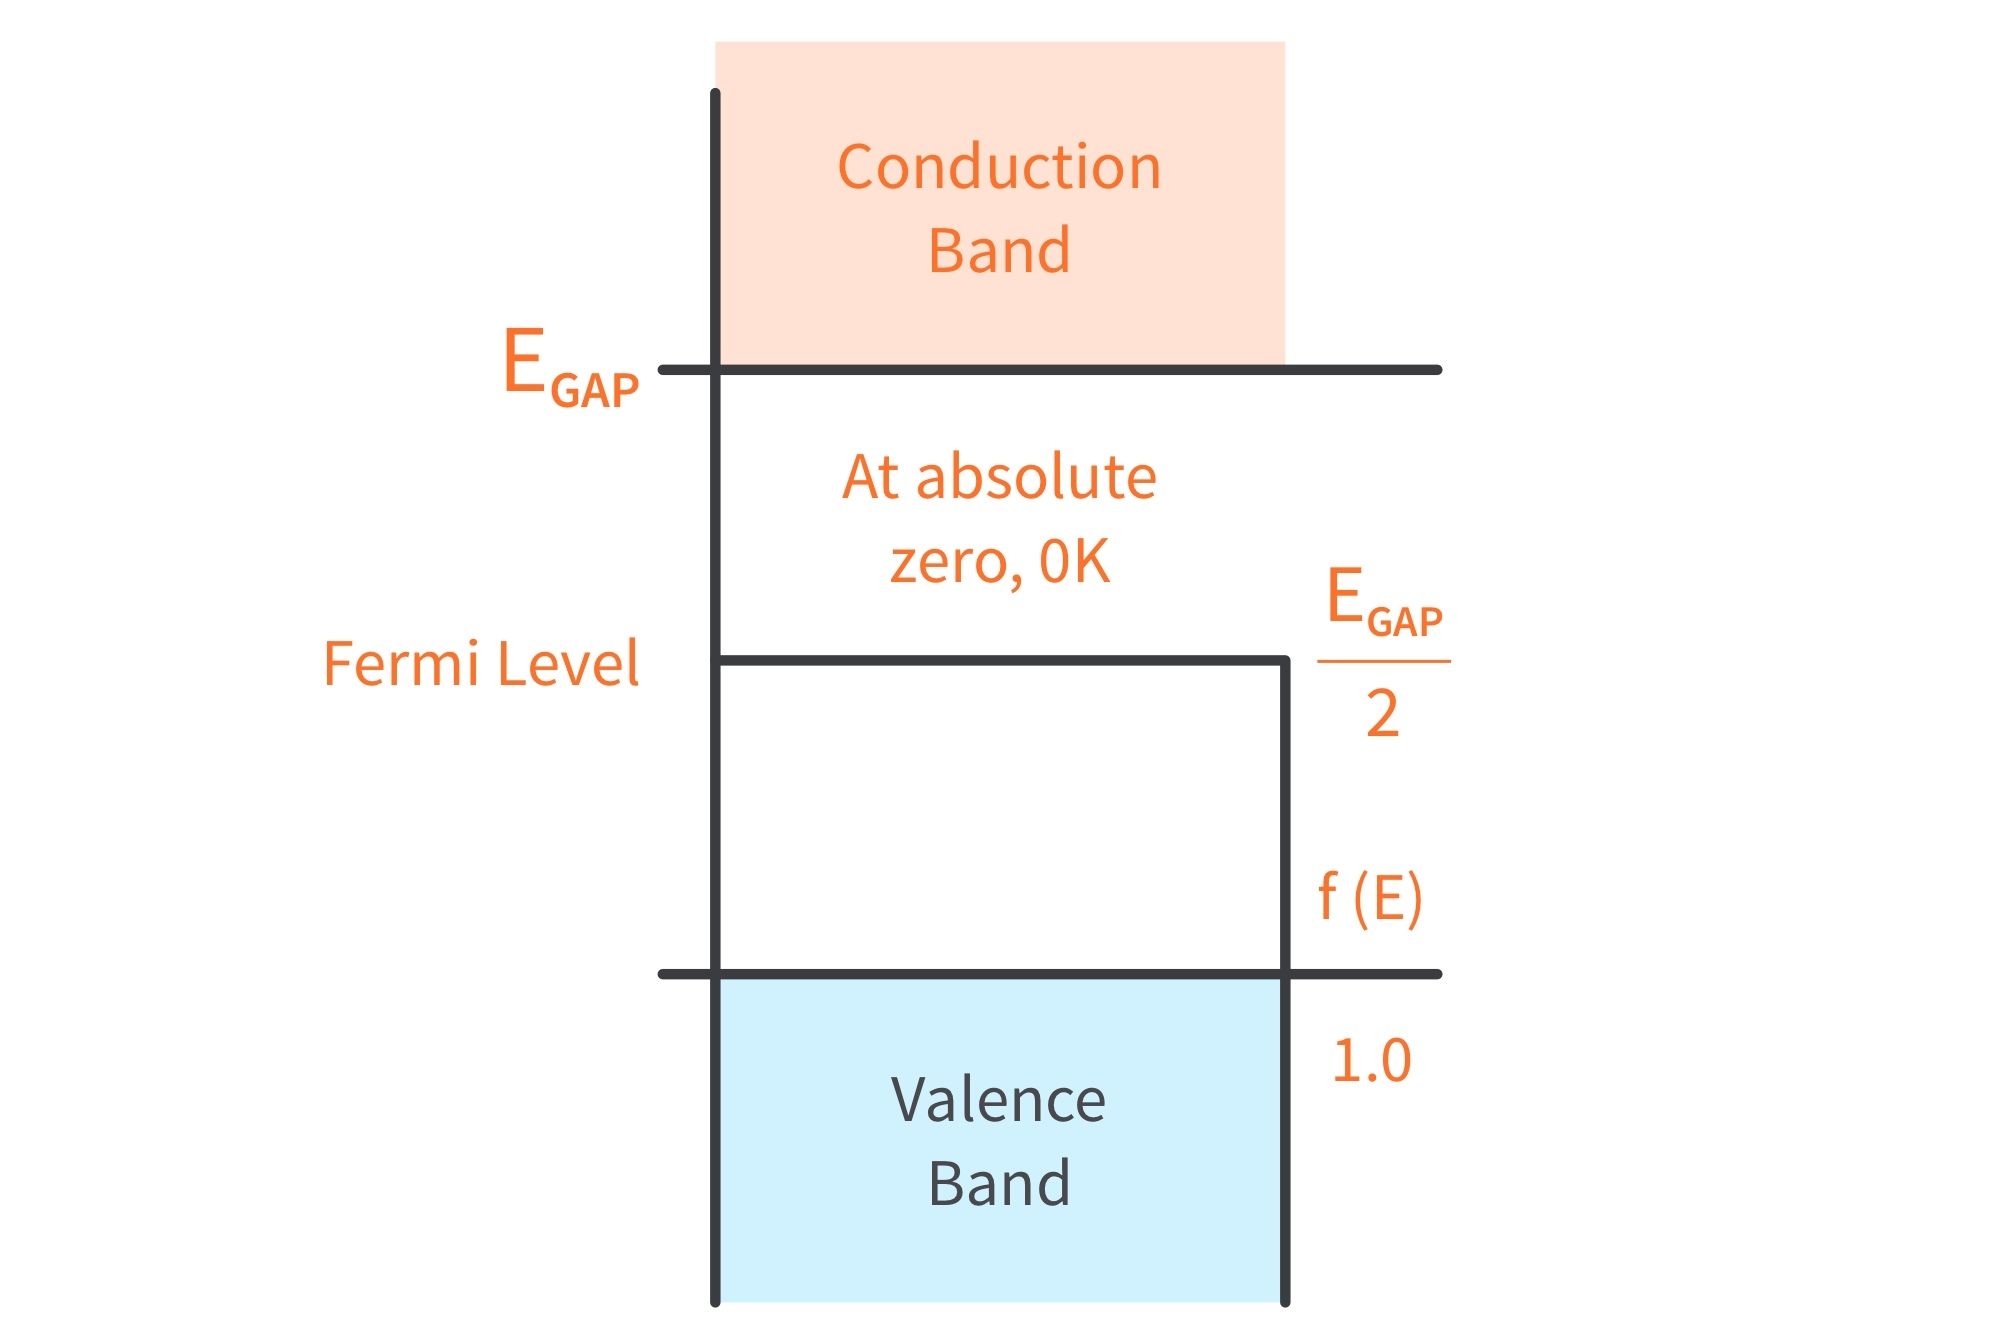
\includegraphics[width=0.3\linewidth]{figures/Semiconductor-Fermi-Level-Band-Diagram-1.jpg}
%     \caption{Tingkatan Fermi pada\\Bahan Semikonduktor}\label{fermilevel}
% \end{figure}
% Apabila ada dua gambar, kita juga bisa menaruh keduanya berdampingan.

% \begin{figure}[H]
%     \centering
%     \subfigure[]{
%         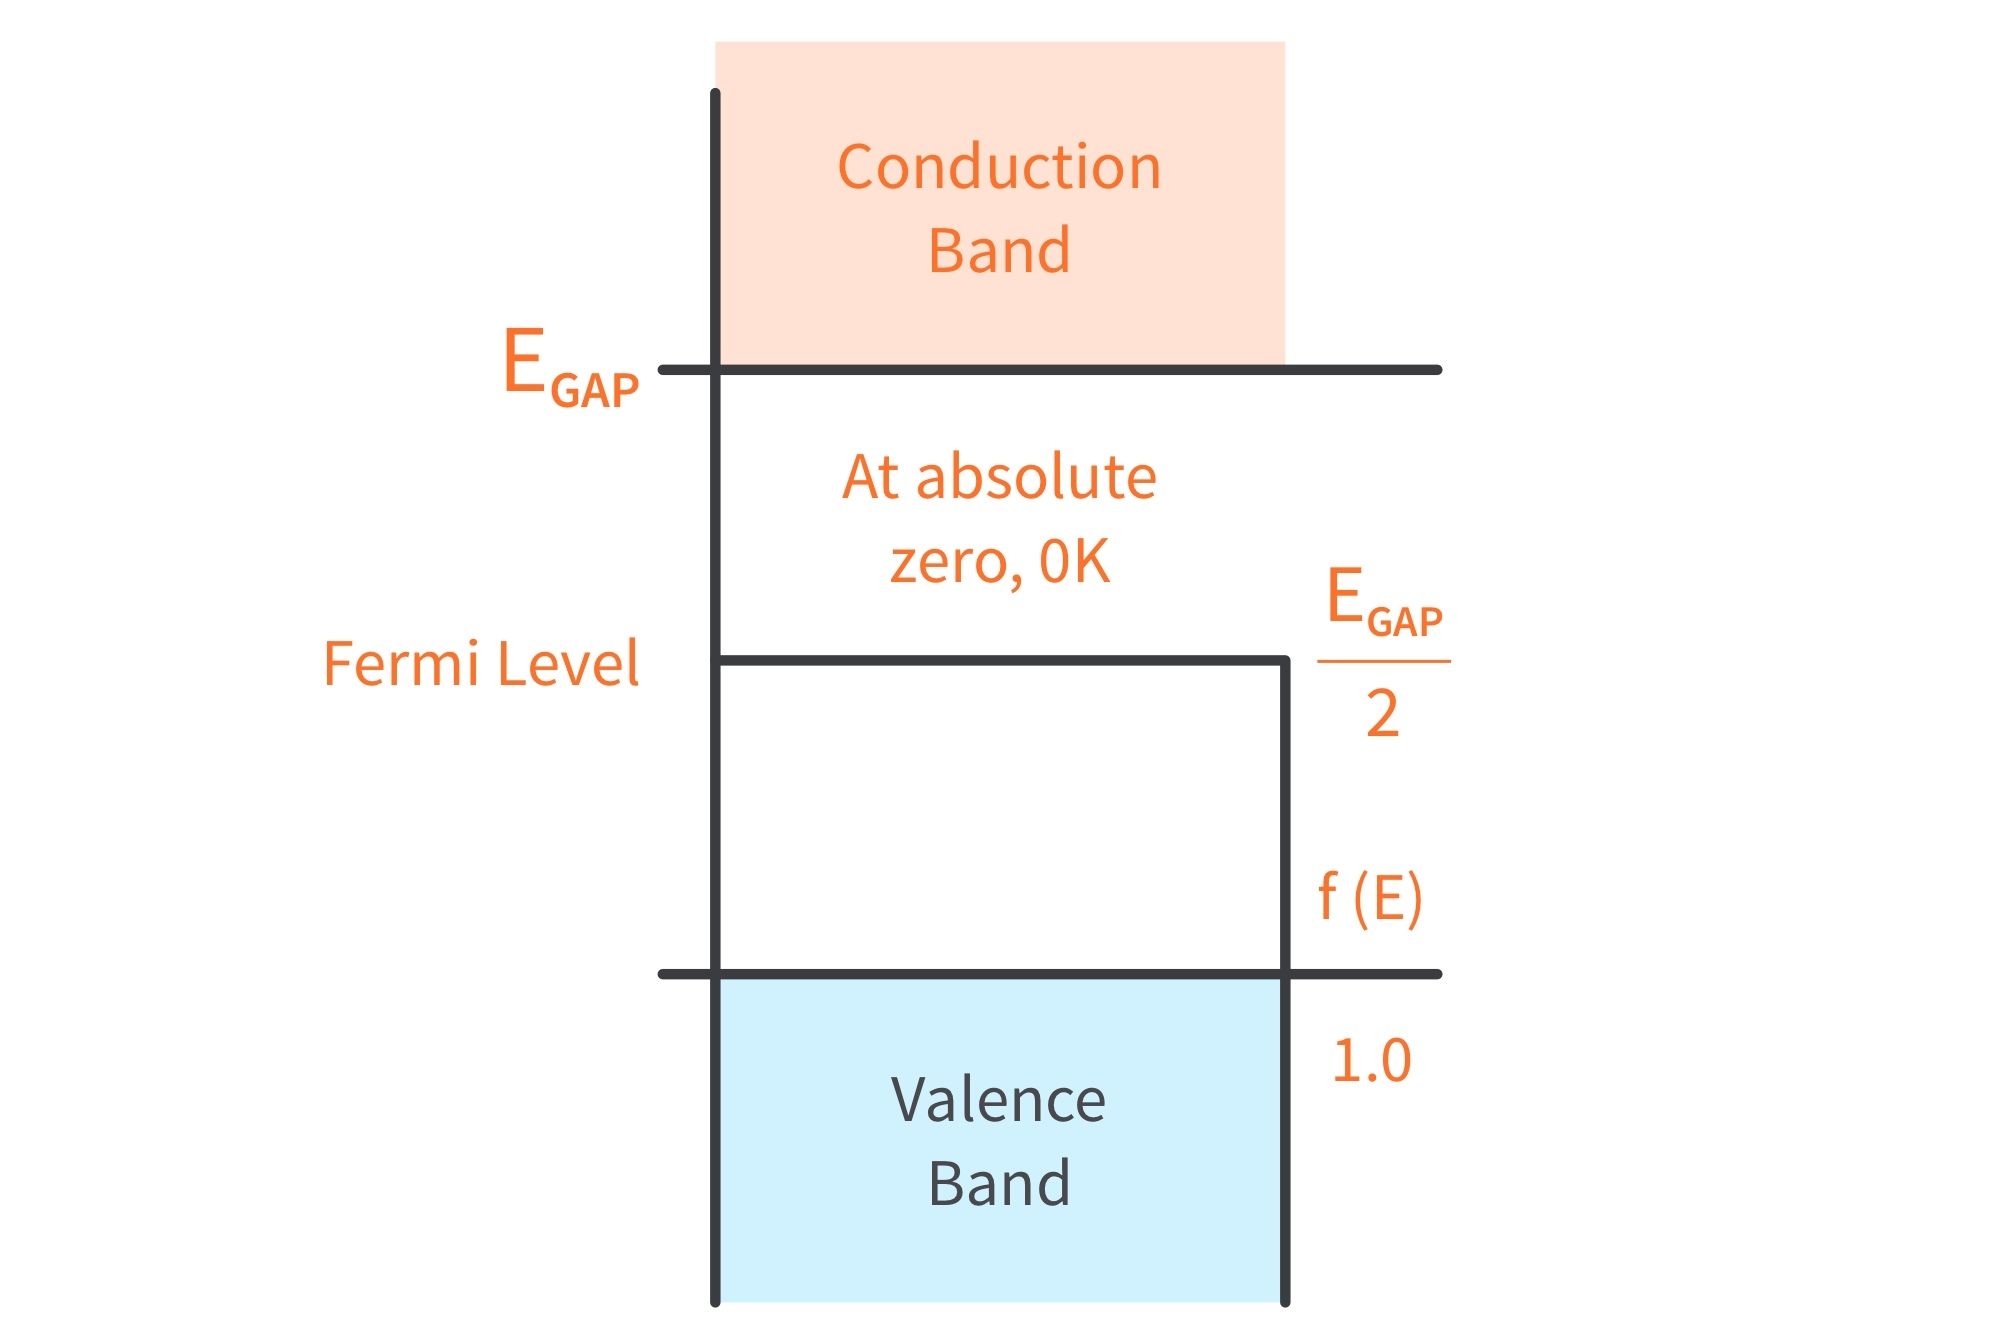
\includegraphics[width=0.4\linewidth]{figures/Semiconductor-Fermi-Level-Band-Diagram-1.jpg}\label{surf-1}
%     }\hspace{0.1\linewidth}
%     \subfigure[]{
%         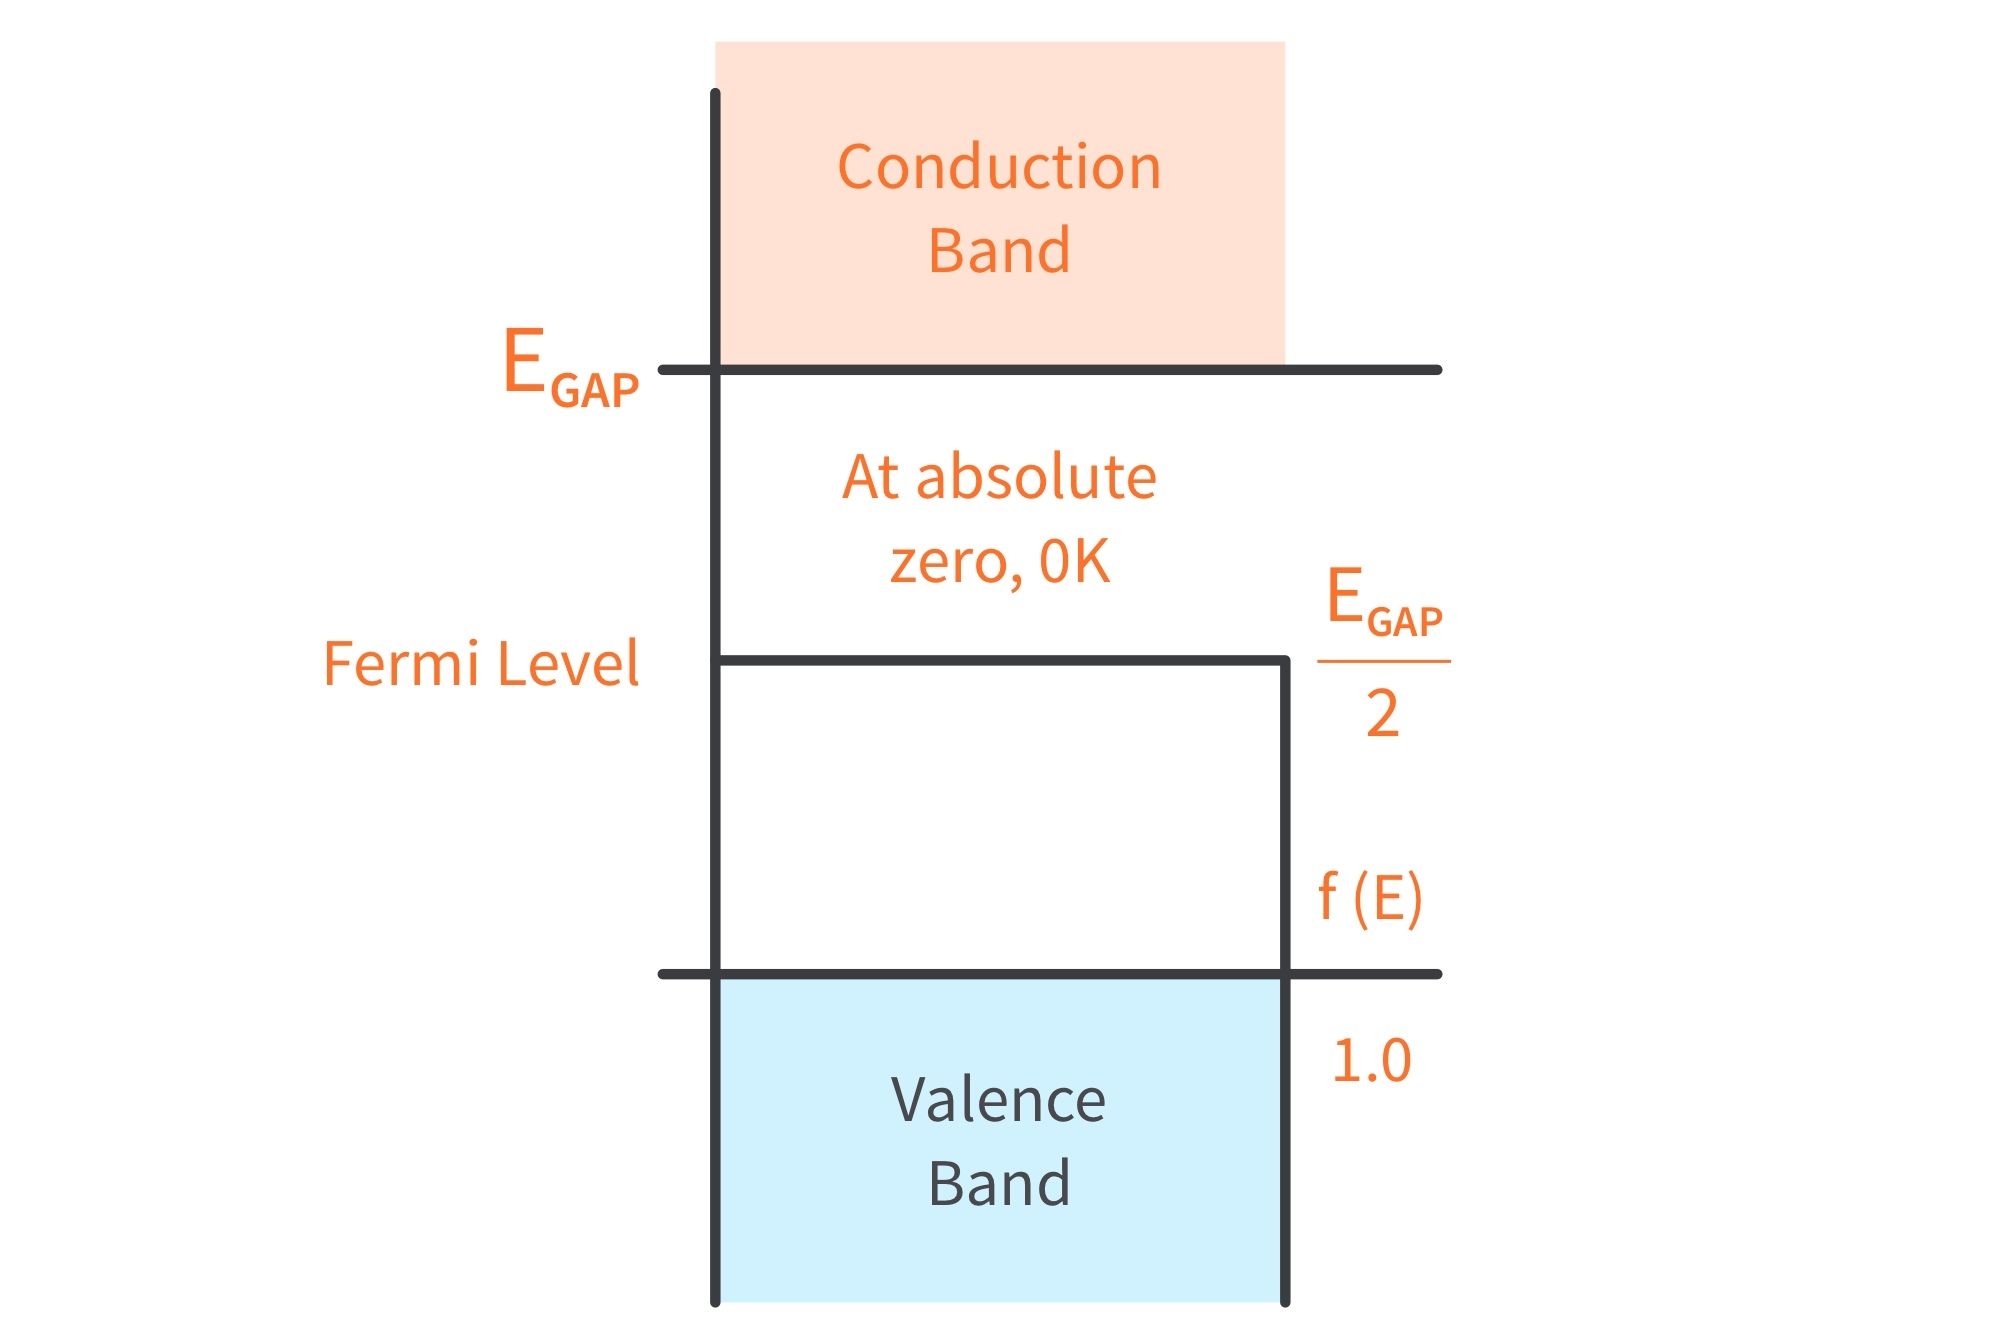
\includegraphics[width=0.4\linewidth]{figures/Semiconductor-Fermi-Level-Band-Diagram-1.jpg}\label{surf-2}
%     }
%     \caption{Dengan menempatkan gambar \subref{surf-1} dan \subref{surf-2}, pembaca akan lebih mudah membandingkan keduanya.}\label{surface}
% \end{figure}
